\documentclass[12pt,a4paper]{report}

\setlength{\parskip}{1em} % Adjust the value as per your preference
\usepackage{tabularx}
\usepackage{booktabs}
\usepackage{geometry}
\usepackage{float}
\usepackage{titlesec}
\usepackage{amssymb,amsmath}
\usepackage[]{graphicx} \graphicspath{ {Fig/} }
\usepackage{caption}
\usepackage[]{xcolor}
\usepackage{booktabs, multirow}
\usepackage{listings}
\usepackage{listings}
\usepackage{color}
\usepackage{minted}

\definecolor{dkgreen}{rgb}{0,0.6,0}
\definecolor{gray}{rgb}{0.5,0.5,0.5}
\definecolor{mauve}{rgb}{0.58,0,0.82}

\lstset{frame=tb,
  language=Python,
  aboveskip=3mm,
  belowskip=3mm,
  showstringspaces=false,
  columns=flexible,
  basicstyle={\small\ttfamily},
  numbers=none,
  numberstyle=\tiny\color{gray},
  keywordstyle=\color{blue},
  commentstyle=\color{dkgreen},
  stringstyle=\color{mauve},
  breaklines=true,
  breakatwhitespace=true,
  tabsize=3
}
 
\usepackage[style=apa]{biblatex} % Move biblatex package here
\usepackage[colorlinks,linkcolor=black,urlcolor=blue,citecolor=blue]{hyperref} % Move hyperref package here
\renewcommand*{\nameyeardelim}{\addcomma\space}
\DeclareFieldFormat{citehyperref}{%
  \DeclareFieldAlias{bibhyperref}{noformat}% Avoid nested links
  \bibhyperref{#1}}

\makeatletter
\renewbibmacro*{cite:labelyear+extrayear}{%
  \iffieldundef{labelyear}
    {}
    {\printtext[bibhyperref]{%
       \printtext[parens]{%
         \printfield{labelyear}%
         \printfield{extrayear}}}}}
\makeatother

\DeclareCiteCommand{\cite}[\mkbibparens]
  {\usebibmacro{prenote}}
  {\usebibmacro{citeindex}%
   \printnames{labelname}%
   \setunit{\space}%
   \printfield{year}%
   \setunit{\addcomma\space}%
   \printfield{postnote}}
  {\multicitedelim}
  {\usebibmacro{postnote}}

\addbibresource{aa.bib} % Specify the bibliography file\usepackage{url}
\usepackage{times} % Set font to Times New Roman
\usepackage{booktabs}
\usepackage{acronym}




\usepackage[english]{babel}  %%% !!! Cancellare 'english' per avere "Sommario, Capitolo..." !!!

%------------------------------------------------------------------------------------
\newcommand{\eg}{\`e}
\newcommand{\ea}{\'e}
\newcommand{\Eg}{\`E}
\newcommand{\og}{\`o}
\newcommand{\ag}{\`a}
\newcommand{\ug}{\`u}
\newcommand{\ig}{\`{\i}}
\newcommand{\R}{\textsf{R}}
\newcommand{\Fortran}{\textsf{Fortran}}
%------------------------------------------------------------------------------------
\definecolor{MyGray}{rgb}{0.,0.,0.} % definizione grigio
\definecolor{MyDarkBlue}{rgb}{0.,0.,0} % blu scuro
\definecolor{MyLightBlue}{rgb}{0.,0.,0} % blu chiaro
\definecolor{MyDarkRed}{rgb}{0,0,0} % rosso scuro
\definecolor{MyDarkGreen}{rgb}{0.0,0,0} % verde scuro
\definecolor{SectionBlue}{rgb}{0,0,0} % blu per sezioni
\definecolor{SubSectionBlue}{rgb}{0.0,0,0} % blu per sottosezioni
\definecolor{SubSubSectionBlue}{rgb}{0.0,0,0} % blu per sottosottosezioni
%------------------------------------------------------------------------------------
\titleformat{\chapter}[display]
  {\color{SectionBlue}\normalfont\LARGE\bfseries}{\chaptertitlename\ \thechapter}{20pt}{\Huge}
\titleformat{\section}
{\color{SectionBlue}\normalfont\Large\bfseries}
{\color{SectionBlue}\thesection}{1em}{}
\titleformat{\subsection}
{\color{SubSectionBlue}\normalfont\Large\bfseries}
{\color{SubSectionBlue}\thesubsection}{1em}{}
\titleformat{\subsubsection}
{\color{SubSubSectionBlue}\normalfont\large\bfseries}
{\color{SubSubSectionBlue}\thesubsubsection}{1em}{}
\DeclareCaptionFont{myblue}{\color{SubSectionBlue}}
\captionsetup{labelfont={myblue,bf}}
%------------------------------------------------------------------------------------
\newcommand{\myboldverb}[1]{{\color{MyDarkBlue}\bfseries{#1}}} % per enfasi in grassetto 
\newcommand{\myverb}[1]{{\color{MyDarkBlue}\texttt{#1}}} % in evidenza
\newcommand{\myurl}[1]{{\color{MyDarkGreen}\url{#1}}} % per url
\newcommand{\quotesection}[1]{{\color{SectionBlue}\textbf{Sezione \ref{#1}}}}
\newcommand{\quotesubsection}[1]{{\color{SubSectionBlue}\textbf{Sezione \ref{#1}}}}
\newcommand{\quotesubsubsection}[1]{{\color{SubSubSectionBlue}\textbf{Sezione \ref{#1}}}}
\newcommand{\quotefigure}[1]{{\color{MyDarkGreen}\textbf{Figura \ref{#1}}}}
\newcommand{\quotetable}[1]{{\color{MyDarkGreen}\textbf{Tabella \ref{#1}}}}
%------------------------------------------------------------------------------------
\geometry{
	paper=a4paper, % Change to letterpaper for US letter
	inner=3cm, % Inner margin
	outer=3cm, % Outer margin
	bindingoffset=0.5cm, % Binding offset
	top=4cm, % Top margin
	bottom=4cm, % Bottom margin
	%showframe, % Uncomment to show how the type block is set on the page
}


%------------------------------------------------------------------------------------
%------------------------------ HERE WE GO ------------------------------------------
%------------------------------------------------------------------------------------


\begin{document}
\title{}
\author{Esterin Kojtari}
\date{8th February 2024}

%----------------------------- Frontispiece
\newgeometry{margin=0.8in}
\begin{titlepage}
    \begin{center}
        \vspace*{0.2cm}
        {\fontsize{19pt}{20pt}\selectfont \textbf{Alma Mater Studiorum - Universit{\ag} di Bologna}\par}
    
        \noindent\hrulefill
        \vspace{0.8cm}
        
        \Large
        
        Department of Political and Social Science
        
        Master's Degree in International Politics and Economics
        
        \Large
        \vspace{5cm}
        {\fontsize{21pt}{20}\textcolor{MyDarkBlue}{\textbf{Exploring the Cyber Dimension of War in Ukraine: Key Lessons for the EU}}}

        
        \vspace{1cm}
        {\fontsize{16pt}{16pt}Thesis in Cybersecurity and International Business}
        
        \vspace{4.5cm}
        \begin{minipage}[t]{0.34\textwidth}
        \begin{flushleft}
        {\fontsize{16pt}{16pt}Candidate: \\ \textbf{\textcolor{MyDarkBlue}{Esterin Kojtari}}}
        \end{flushleft}
        \end{minipage}
        \begin{minipage}[t]{0.64\textwidth}
        \begin{flushright} \Large
        Supervisor: \\
        \textbf{\textcolor{MyDarkBlue}{Chiar.mo Prof.}} \\ \textbf{\textcolor{MyDarkBlue}{Luigi Martino}} 
        \end{flushright}
        \end{minipage}\\
        
        \vfill
        \noindent\hrulefill
        \vspace{0.3cm}
        \Large
        
        Appello {\textcolor{MyDarkBlue} {IV}} 
        
        Anno Accademico {\textcolor{MyDarkBlue} {2022-2023}}
    \end{center}
\end{titlepage}
\restoregeometry
\vspace*{5cm}

% dedicaation
%\begin{flushright}
 % {\parbox{4.2cm}{\textit{Dedication}}}
%\end{flushright}

\thispagestyle{empty}
%\newpage
%-------------------------------------ABSTRACT
%\thispagestyle{empty}
\vspace*{5cm}
\renewcommand{\abstractname}{\color{MyDarkBlue}{Abstract}} 
\begin{abstract}
In the evolving landscape of global security, the intersection of technology, warfare, and international relations are reshaping geopolitical dynamics. This dissertation explores the intricate dynamics of cyber defence by focusing on the Russia-Ukraine War within the broader context of the European Union's cybersecurity framework. Using a multidisciplinary framework that encompasses international relations, cybersecurity, European law, and programming languages for data analysis, this study adopts a mixed-method approach. Integrating qualitative and quantitative analyses, the research aims to uncover the complex landscape of cyber-related phenomena. Guided by theoretical concepts like Complex Interdependence, Securitisation Theory, and Neo-Functionalism, the study offers a lens to interpret cyber power dynamics and evolving state interactions in the digital age. In the first part, the study delves into the cyber dimension of the Russia-Ukraine conflict, unraveling the strategies employed, and lessons learnt. The second part shifts focus to the European Union and its members, conducting a comparative analysis of cybersecurity approaches in France, Estonia, Germany, and the Netherlands. Insights from Russian cyber operations highlight the need for a resilient strategy in critical infrastructure defence and the challenges in investment for skill development and infrastructure enhancement. Notably, the EU emerges as a normative cyber power, influencing cyber capabilities among its Member States, acting as a catalyst in shaping ongoing cyber strategies within the civil sphere rather than the military domain. The comparative analysis reveals diverse approaches in political initiatives, deterrence, economic measures, and military domain. Challenges have been underscored, including the skill gap and the need for collaboration between the public and private sectors. However, the integration with military kinetic counterparts is yet to be substantially realised.

\vspace{1cm}
\noindent\textbf{Keywords}: Cyber Operations, European Union Cyberstrategy, Ukraine-Russia War, Cyber Defence, Cyber-Kinetic Military Integration
\end{abstract}
%-------------------------------------INDEX
\setcounter{page}{1}
\pagenumbering{roman}
\tableofcontents{}
\listoffigures{}
\listoftables{}
%\vspace*{2cm}
%\setcounter{page}{1}
%\pagenumbering{arabic}



%%%%%%%%%%%%%%%%%%%%%%%%%%%%%%%%%%%%% Chapters
\setcounter{page}{1}
\pagenumbering{arabic}
\chapter*{Introduction}
\phantomsection
\addcontentsline{toc}{chapter}{Introduction}


\begin{quote}
\centering
--------------------------------------------------------------------------------- \\
If you spend more on coffee than on IT security, you will be hacked.
\\ - Richard A. Clarke
--------------------------------------------------------------------------------- \\
\end{quote}

Today's world is characterized by rapid technological advancement and interconnected global networks, wherein the security landscape is constantly evolving. The cyber domain, as a cross-cutting sphere, serves as a meeting ground for international actors, private companies, and non-state entities, where collaborations and occasional struggles unfold. The absence of a deterministic international law applied to govern and prevent escalation leads to a chaotic and unexpected outcome in the real world.

In recent times, scholars' attention to cybersecurity issues has significantly increased. Cyber issues are no longer marginalised in academic discussions and are not solely viewed through the lens of security from an Anglo-Saxon perspective. However, the academic community has yet to reach a consensus on the fundamental concepts of the matter; theories, frameworks, and analyses have been produced with significant results, laying the groundwork for the future growth of this domain.

This research delves into the dynamics of cyber defence by analysing how cyber operations are conducted, focusing on the Russia-Ukraine War, European Union and its Member States. 

This research project will exploit the characteristic and the outcomes of the Russian invasion of Ukraine, analysing it from a cybersecurity perspective to takeaway insights and lessons from the first interstate war in the information age. 

The research will encompass a multidisciplinary approach drawing on insights from International Relations, Cybersecurity, European Law and data analysis through programming languages (\textit{python}). Specifically, the research gathered data from dataset such as the European Repository of Cyber Incidents (EuRepoC) and Cyber Operations Tracker from Council on Foreign Relations. 

The theoretical framework of the research draws on concepts such as Complex Interdependence, Securitisation Theory, and Neo-Functionalism, providing a lens through which to analyse the multifaceted nature of cyber-related phenomena. Each theoretical perspective contributes unique insights to the understanding of cyber power dynamics, the securitisation process, and the evolving nature of state interactions in the digital age.

The subsequent chapters navigate through critical aspects of cyberspace, exploring key terms, assessing cyber power, and examining the significance of cyber defence. The research further investigates the cyber dimension of conflicts, specifically focusing on the Russian invasion of Ukraine, where the cyber realm constitute a real threat. It sheds light on intelligence gathering, the role of hacktivists, and the lessons to be learned from the cyber operations during wartime.

The latter chapters transition towards a European perspective, evaluating the EU's historical cyber strategy, cooperation mechanisms between institutions and member states, and the overarching theme of digital sovereignty. The research culminates in a comparative analysis of European countries—France, Estonia, Germany, and the Netherlands—assessing their preparedness for cyber operations.

In conclusion, the comparative analysis underscores diverse approaches to cybersecurity, shaped by the lessons learned from the Ukraine conflict. Economic measures, critical infrastructure protection, and military integration are identified as crucial pillars for cybersecurity resilience across these nations. Challenges such as the skills gap and public-private sector cooperation persist, prompting tailored initiatives and collaborations. The lessons drawn from the war in Ukraine emphasise the necessity for flexibility, collaboration, and adaptability in the face of emerging cyber threats. The commitment of these European nations, guided by ongoing processes to increase cyber preparedness, signifies their active engagement in shaping the future effectiveness of their cybersecurity efforts. 
\chapter{Methodology}

This chapter examines the methodology used in the study, focusing on the impact of cyber operations in Ukraine on the EU cybersecurity framework. The methodological chapter is structured to provide an understanding of the complex relationship between cyber operations, warfare, and cybersecurity policy at national and EU levels The chapter will cover the research design, compilation and description of datasets to be used. In addition, it will describe the methods used to analyse data, its integrity and reliability, and the conduct of a qualitative document review.

\section{Research Desing}

The goal of the study is to investigate the cyber aspect of the conflict in Ukraine and collect important lessons for the cyber strategy of the European Union. In order to accomplish this goal, a study of the cyberwar in Ukraine from both the Ukrainian and Russian perspectives will be conducted, revealing the strategies employed to deter cyberattacks during wartime. Then, these methods will be researched on Estonian, French, German, and Dutch national cybersecurity policies. We will additionally investigate how the European Union may act as a catalyst for better cybersecurity among its Member States by encouraging and supporting the adoption of these strategies.

This research will employ a mixed-methods approach. The decision to proceed with both qualitative and quantitative analysis is informed by the complex and multifaced nature of our research question and domain. The quantitative data will provide us with statistical rigour with the aim of identifying patterns and correlations between observations. On the other hand, the qualitative analysis will help us to contextualise and interpret observed data. Qualitative methods, such as normative content analysis and case studies, will be used in our analysis. 

The research will be divided into two parts. The first will focus on the cyber dimension of the war in Ukraine, where it will serve as a case study to analyse the adoption of cyber operations during wartime. It will investigate the methods, objectives, and effects of cyber operations.  

The second part will delve into the analysis of the European Union and its Member States. Its position will delight its status as a cyber power and the current efforts to build a cyber defence for its Member States. The different methods of cyber defence within the European Union will also be addressed by comparing France, Germany, the Netherlands, and Estonia. The comparative analysis will take into consideration factors such as the national institutions on cybersecurity issues, EU-sponsored projects under the Permanent Structured Cooperation (PESCO) and insights from previous cyberattacks.

The reason for the selection of these countries lies in their strategic role in cyber defence within the European Union, even with different approaches. The strategic differences represent a spectrum between experienced cyber defenders (Estonia) and major players in EU politics (Netherlands, France, and Germany). Additionally, these nations present a rich repository of official documents and publicly accessible data, significantly contributing to our research.

\section{Research Type}

Our work falls within the category of interpretive research. We aim to not only describe and understand the key lessons learned, but also explain why these lessons are essential for shaping future strategies. The interpretive research is well-suited for emerging fields such as cyber politics during wartime. A flexible and open-ended research method as well as a multidisciplinary approach are required due to the complexity of the area. The interpretative research will not find the causal phenomena for generalizable law-like regularities \autocite{lamont_2021_research}, instead, the focus will be on understanding the interaction between politics and technology in a fast-paced world.

\section{Data Collection}

When studying cybersecurity issues, one of the biggest challenges that scholars and researchers must tackle is associated with data availability. Different factors affect the availability of data on cyberattacks, perpetrators, and victims. \textcite{cremer_2022_cyber} analysed 5219 cyber peer-reviewed studies and found that only 79 unique datasets were used. First, cybersecurity, like other security-related areas, is hidden behind states' or companies’ secrets. The state is not always open to disclosing attacks on its critical infrastructure, which undermines its popularity among citizens. However, cyberattacks undermine their reputation. Even in most countries, there are some binding rules to inform companies’ clients about data breaches or other types of attacks; information about attacks is fragmented and incomplete. Another reason relates to the nature of cyber-capabilities. Before being discovered or starting to produce some effects, a malicious attack vector can hide for an indefinite time. For instance, Stuxnet, a highly sophisticated cyberattack, was concealed through a combination of intricate techniques and targeted strategies to attack Iran's uranium-enrichment centrifuges. The gradual and methodical approach that Stuxnet took in damaging the centrifuges allowed it to operate silently within Iran's nuclear facilities for several years before it was uncovered. Its inadvertent spread beyond its intended target in 2010 led to this discovery. 
Furthermore, the number of cyberattacks is increasing exponentially, posing a challenge for researchers who may struggle to trace and analyse all of them. 

Moreover, there is a lack of open-source databases containing information on cyberattacks \autocite{cremer_2022_cyber}. Many companies specialising in cyber threat intelligence, including Recorded Future, CrowdStrike, and Fortinet, among others, often refrain from publicly sharing such data because of their business models. However, open-source databases could help practitioners and companies facilitate data gathering and sharing to develop and upgrade their best practices to mitigate cyberattacks. In addition, an open-source database of cyberattacks could contribute significantly to increasing societal awareness of cyber issues. 

Some steps in this direction have been taken by \textit{open-source intelligence} (OSINT) communities, which actively work to collect and share cyber incident information. These efforts play a crucial role in increasing transparency and knowledge in cybersecurity. 
Two datasets will be used for this purpose of the research project: the \textit{Cyber Operations Tracker} created by the Council on Foreign Relations and the EU Database from the \textit{European Repository of Cyber Incidents} (EuRepoC). 

The use of two different datasets for statistical analysis is essential for several reasons. First, it helps validate and cross-verify findings, reducing the risk of drawing incorrect conclusions from potentially biased or incomplete data. Second, it allows for a more comprehensive analysis by providing diverse perspectives and insights, thus enabling a deeper understanding of the subject. In addition, it facilitates comparative analysis, enabling researchers to explore variations and trends across different datasets, which can lead to more robust and reliable research outcomes.

\newpage
\textbf{Cyber Operations Tracker}

The \textit{Cyber Operations Tracker} developed by the Council on Foreign Relations, an independent think tank, tracks state-sponsored cyber operations which have been disclosed publicly from 2005 to nowadays. The dataset does not include hacktivists' actions and other threat actors that are not engaged in denial-of-service attacks, espionage defacement, destruction of data, sabotage and doxing \autocite{councilonforeignrelations_2023_tracking}. The sources of the attacks are available openly and mentioned in the dataset itself. The Council on Foreign Relations updates the dataset quarterly. As mentioned in their methodology, there are some limitations for the dataset \autocite{councilonforeignrelations_2023_tracking}:

\begin{itemize}
    \item \textit{Attribution}: due to the nature of cyber operations and deceptive tactics from threat actors, attributing the attack to an entity is a challenge. Even though, the dataset includes multiple sources, from technical sources to government websites. However, it remains a contentious issue.
    \item \textit{Data Completeness}: as argued in the previous section, no datasets could be comprehensive to track every cyber (operations) attack. The perpetual change of the techniques and strategies of cyber operations makes the research more difficult.
\end{itemize}

\textbf{EuRepoC}

The \textit{European Repository of Cyber Incidents} (EuRepoC) is an independent research consortium that provides a well-structured overview of cyber incidents with detailed information from 2001 to nowadays. The consortium was established in 2022 by researchers at the University of Heidelberg, the Cyber Policy Institute, the University of Innsbruck and the German Institute for International and Security Affairs (SWP). The EuRepoC dataset combines three coding processes: technical coding by IT forensic experts evaluating various aspects of cyber incidents, political coding by experts focusing on political attribution and responses, and legal coding by legal experts assessing the legal impact and justification of response options, including evidence for sanctions. 

The EuRepoC dataset's data selection criteria involve focusing on publicly reported cyber incidents that have affected political or state actors, have been associated with state actors, or have been publicly politicized. This approach deliberately excludes cases that concern specific stakeholders but are not prominently addressed by political actors. Additionally, the dataset includes a cyber intensity scale that assesses the coded incident types, their potential physical effects, and socio-political severity, assigning a weighted score ranging from 1 to 15 to provide a comprehensive evaluation of each incident's impact and significance.

Both datasets are similar in their approach, and most of the data overlaps. However, the choice to analyse both is useful to understand both a global (with Cyber Operations Tracker) and European (with EuRepoC) perspective of cyberattacks. In addition, the EuRepoC gives us information on whether the attack has caused disruption or not, which is useful to compare the ability of countries to counter the attacks. 

Furthermore, for insights on cyber operations in Ukraine, data from non-governmental organizations (NGOs) such as the CyberPeace Institute and technology companies such as Microsoft and Google (Mandiant). The reason for using data from such sources is linked to their involvement in the cyber defence in Ukraine. Specifically, CyberPeace Institute has developed a project which discovers cyberattacks that aim at civilians while assessing their impact. In addition, Microsoft and Mandiant, among other companies, have contributed to the technical cyber defence of Ukraine against Russian cyber operations \parencite{huntley_2023_fog, smith_2022_defending}.

Moreover, other data from cyber indexes will be used to assess the cyber power of selected EU countries. 




To assess the cyber power and capabilities of the selected European Union countries (France, Germany, the Netherlands, and Estonia) and to facilitate comparative analysis, you have chosen several cyber-related indexes:


\textbf{National Cyber Power Index}

The \textit{National Cyber Power Index} developed by the Belfer Center for Science and International Affairs at Harvard Kennedy School was published in 2020 and updated in 2022. The index evaluates various objectives, including surveillance of domestic groups, enhancing national cyber defences, controlling the information environment, foreign intelligence collection, advancing technology competence, disrupting adversary infrastructure, setting international cyber norms, and accumulating wealth or cryptocurrency. These objectives provide a holistic assessment of a state's cyber capabilities, enabling scholars to analyse them in conjunction with other national tools, such as military and diplomatic means, for pursuing national interests. 

\textbf{Cyber Arms Watch}

The Cyber Arms Watch's \textit{Cyber Transparency Index,} developed by The Hague Centre for Strategic Studies, and published in 2022, evaluates the transparency of a state's cyber offensive capabilities using two main components: the Declared Capabilities Rating (DCR) and the Perceived Capabilities Rating (PCR). The DCR assesses how much a state publicly discloses about its offensive cyber capabilities, while the PCR gauges the perceived capabilities based on external sources. These ratings create the Cyber Transparency Index, which categorizes 60 countries' cyber transparency, including European nations and major international actors. Differently from the other index that included diplomatic and economic cyber power instruments, the Cyber Arms Watch focuses exclusively on offensive cyber capabilities. 


\textbf{National Cyber Security Index}

The \textit{National Cyber Security Index} (NCSI) measures the preparedness of countries to counter and manage cyber threats. It aligns with national cybersecurity frameworks and focuses on measurable aspects of cybersecurity implemented by central governments. The NCSI employs structured categories, capacities, and indicators, all assigned values reflecting their importance. These categories are the general cybersecurity indicators, such as policy development and threat analysis; the baseline cybersecurity indicators, such as the protection of digital and essential services; and incident and crisis management. Country ratings are based on publicly available evidence like legal acts and official documents. The NCSI Score represents a country's performance relative to the maximum, scaled to 100\%. It also includes the Digital Development Level (DDL) to show the relationship between cybersecurity and digital development. In addition, data is collected through government contributions, organizations, individuals, and the NCSI team, with rigorous expert reviews. The NCSI is continually updated for accuracy and relevance.

\begin{table}[htbp]
  \centering
  \caption{Comparison of Cybersecurity Indexes}
  \begin{tabular}{p{1.2cm}p{2.5cm}p{2.5cm}p{2.2cm}p{2.2cm}p{3cm}}
    \toprule
    \textbf{Index Name} &
    \textbf{Objective} &
    \textbf{Data Source} &
    \textbf{Publication Year/Update Frequency} &
    \textbf{Limitations} &
    \textbf{Relevance to Research} \\
    \midrule
    \textit{National Cyber Power Index} &
    Assess cyber capabilities &
    In-house data, proxies &
    2022/Updated regularly &
    Difficulty in data collection for certain objectives &
    Evaluate cyber capabilities \\
    \midrule
    \textit{Cyber Arms Watch} &
    Analyze transparency of cyber offensive capabilities &
    The Hague Centre for Strategic Studies &
    2022 &
    Challenges in assessing transparency &
    Measure transparency and disclosure \\
    \midrule
    \textit{Nation Cyber Security Index}&
    Measure preparedness to prevent cyber threats &
    Publicly available evidence materials from governments, organizations, and individuals &
    2016/ (Continuous process) &
    Data collection and public evidence-based assessment &
    Assess national cyber security preparedness \\
    \bottomrule
  \end{tabular}
\end{table}


The relevance of the indexes will not be on the rankings or the numerical value for each country. Rather, the picture that those indexes represent. Those indexes, even with different approaches, are powerful tools in situations in which retrieving information from sectors where its security is a must. 

\section{Data Analysis Methods}
\subsection{Data processing}

Data pre-processing will be carried out using Python in Jupyter Notebooks, and all \textit{.csv} and \textit{.ipynb} files will be made freely available on \textit{GitHub}, where the documentation for each Python script will be present. We will utilize Python libraries such as Pandas, Matplotlib, Seaborn, Folium, Plotly, NetworkX, and natural language processing tools to bolster our data analysis and visualization efforts.

To narrow our focus to the selected countries, we will filter both cyberattack datasets. For the Cyber Operations Tracker database, where country references are absent and only entities or institutions are mentioned, we will leverage natural language processing techniques to isolate the designated countries. Additionally, columns with null data will be removed. A consolidated dataset will be created to incorporate the indexes mentioned earlier, and it will be merged with statistics gathered from national authorities, ENISA, and European institutions (such as PESCO projects, investments in ICT and others). We aim to investigate the methods, objectives, and effects of cyber operations in this context, shedding light on the evolving landscape of cyber warfare in the region.

For the effective visualisation and communication of our research findings, we will employ various scripts to create maps, network diagrams, and statistical plots. Statistical methods, such as regressions and correlations, will be carried out with the aim of finding relevant patterns and insights on our exploratory data analysis.


\subsection{Data Validity and Reliability}

To ensure the quality of data, the research presents only reliable and trusted sources, avoiding speculations. The data pre-processing will enhance the validity of our datasets while handling missing values. In addition, the interpretation of the data will be supported by the literature review. 

\subsection{Qualitative Document Analysis}

The content analysis will be conducted on European official documents obtained through EUR-Lex. The documents will be classified according to their nature (regulations, directives, information among others), and analysed with the aim to explore EU objectives and priorities, policy measures and reference to the cyber capabilities. 
The list of documents to analyse is present in the Annex. The analysis will start from 2014, the year of the first Cybersecurity Strategy of the European Union, to 2023. For achieving a systemic analysis, we will use a common framework for each of the documents presented in Table \ref{tab:framework-elements}

\begin{table}[ht]
\centering
\caption{Framework Elements for Analyzing EU Cybersecurity Documents}
\label{tab:framework-elements}
\begin{tabular}{|c|p{8cm}|}
\hline
\textbf{Framework Element} & \textbf{Description} \\
\hline
\multirow{2}{*}{\textit{Document Classification}} & Categorize documents based on their nature (e.g., regulations, directives, reports, strategies). \\
& \\
\hline
\multirow{2}{*}{\textit{Objectives and Priorities}} & Extract stated objectives and priorities outlined in the documents. Consider overarching objectives and specific cybersecurity goals. \\
& \\
\hline\textit{}
\multirow{2}{*}{\textit{Cyber Capabilities}} & Examine references to the EU's cyber capabilities. Look for mentions of cybersecurity capabilities in terms of defense, response, and deterrence. \\
& \\
\hline
\multirow{2}{*}{\textit{Roles and Responsibilities}} & Identify roles and responsibilities assigned to EU bodies, member states, and stakeholders in implementing cybersecurity measures. \\
& \\
\hline
\multirow{2}{*}{\textit{Resource Allocation}} & Investigate how the documents address resource allocation for cybersecurity initiatives. Consider budgetary provisions, funding mechanisms, and priorities. \\
& \\
\hline
\multirow{2}{*}{\textit{Challenges and Threats}} & Identify challenges and emerging threats mentioned in the documents. Consider the EU's plans to address these challenges and adapt to new threats. \\
& \\
\hline
\end{tabular}
\end{table}

\section{Limitations}

What do information on cyberattacks, the use of cyber tactics, and how indexes are made have in common? The frequent difficulty in obtaining thorough, current information. Cyberspace, which is human-made, provides the perfect setting for keeping a lot of information secret. In fact, the secrecy surrounding such actions frequently makes it difficult for academics to locate trustworthy sources and data. 

The countries that were chosen are those that promote greater transparency in government files. This method, however, presents a geographical bias because these states cannot be seen as unique role models for the European Union but rather as the most cyber-developed countries in this area.

However, it is crucial to delight some of the problems for research in the cyber domain, particularly concerning the application of cyber operations during wartime with the Ukraine War case. The limitations of this work are reflected in the availability of data. Both parties involved in the conflict were restrained from sharing them. In addition, the \textit{Cyber War Fog} could affect the objectivity of critical analysis. The Ukraine–Russia war could lead to imperfect empirical knowledge of a single historic event.  Despite all the limitations, this research could serve as a springboard for further investigation into the Ukrainian conflict's cyber dimension, which will serve as a foundation for other studies on cyber operations in times of war.

\section{Ethical Considerations}

All information and data gathered for this research are freely available on the internet. Due to sensitive information that cyber operations involve, the research will not use potentially classified data, but rather will use only open-source data and peer-reviewed information. 





\chapter{Theoretical Framework}

Our theoretical foundation to pursue this research will be based on three different theories in International Relations. The complex interdependence and subsequently weaponization of the interdependence will explore the role of cyberspace in the hyper-globalised world and the growing relevance of non-state actors. Next, we will apply securitization theory to cyberspace, now recognized as the fifth battlefield, where zero-sum games are played. Finally, the institutionalism theory will explain why the European Union is relevant in shaping the member states cyberstrategies and how it is contributing to set new rules for the other actors. 

\section{Complex Interdependence and its weaponization}

The theory of Complex Interdependence was minted by Joseph Nye and Robert Keohane in the 1970s with their book Power and Interdependence. They understood that transnational political issues were linking states. Specifically, they focused on the flows of transactions, goods, and services to create boundaries in the international arena. As \textcite{nye_1971_transnational} asserted, the theory of Complex Interdependence is characterised by:

\begin{enumerate}
    \item \textbf{Multiple channels between actors}: These channels encompass diplomatic, economic, social, and technological interactions.
    \item \textbf{Absence of hierarchy}: new actors move in the international arena, such as the Non-Governmental Organisations. 
    \item \textbf{Minor role of Military force}: while military power remains important, it is not the only one for pursuing the state’s interests. 

\end{enumerate}

In the information age and an ever-more globalised world, the channels through which Complex Interdependence operates have significantly expanded and evolved. These transformations have profoundly reshaped the dynamics of international relations. Interdependence can be weaponised by one of the actors. In the context of cyberspace today, even small states and non-state actors can render larger states vulnerable \parencite{farrell_2019_weaponized, nye_1971_transnational}(Farell and Newmann, Nye and Keohane). Nowadays, cyberspace constitutes the basis of any economy in the world, from international trade to financial transactions and public information. All data is no longer physically stored in folders but in the cloud database, thus reducing transaction costs. Although theoretically, each actor could take advantage of these technological innovations, these benefits are distributed non-homogeneous among them. The US, Russia, China, and the European Union are the major international powers from the technological infrastructures' perspective, as well as the ability to create leading international companies in the tech sector. Digital Information and Communication Technology (ICT) and technological innovations are the main reasons for the rapid spread of global supply chains \autocite{mansfield_2021_embedded}, fortifying interdependence and enhancing productivity. Different poles of cyber power but interdependent with each other. Interdependence is structured from the material perspective (China is the leading exporter of rare earth elements, indispensable for constructing semiconductors) and technological know-how. Indeed, this work will go beyond the liberal complex interdependence by affirming that network interdependence provokes power imbalances among states; consequently, asymmetric network structures create the potential for weaponised interdependence \autocite[45]{farrell_2019_weaponized}. Cyberspace and its physical infrastructures are asymmetric distributed and decentralised networks, but state actors are using its interdependence to project their power. However, cyberspace weaponisation is possible only for privileged actors who control hubs (physical such as satellite and submarine cables and online as servers) and have domestic institutions with the cyber capabilities to intervene \autocite{farrell_2019_weaponized}.

\section{Securitisation Theory}

The concept of securitisation was developed by the Copenhagen School as one of the milestone of security studies discipline. In 1998, Barry Buzan, Ole Wæver, and Jaap de Wilde published "Security: A New Framework for Analysis," which not only defined the concept of security but also continues to shape it to this day. This concept of securitisation has an intersubjective meaning, where a state can socially construct a threat, even if it is not necessarily reflected by the objective, material circumstances of the world \autocite{balzacq_2016_securitization}. This approach has been applied to other areas such as the economy, energy, and environmental issues, where each sector poses a threat to a referent object, such as identity or ecosystem \autocite{eroukhmanoff_2018_securitisation}. The fundamental aspect of the theory lies in the capacity of political discourse, a speech act, to not just describe reality but to constitute it. 

In the digital era, cyber constitutes another field where securitisation has been applied.  Scholars such \textcite{hansen_2009_digital} have assumed that this new field has experienced \textit{hypersecuritisation} since the dystopic futures described in the pop culture about cyber doom day. The literature highlights the new capacity of non-state actors to have similar \textit{cyber-fires} of states and moreover, the possibility of individuals to have a say, without underestimating the network that englobes all the actors. 

With this regard, \textcite{lacy_2018_securitization} have defined three different positions that shape the securitisation of cybersecurity.

\begin{itemize}
    \item \textbf{Cyber Catastrophist}: This perspective asserts that there's a genuine risk of digital catastrophes that could cause major societal, economic, and infrastructure problems. It contends that discussions about geopolitical threats often downplay the significance of cyber threats and caution against potential events akin to \textit{cyber 911s} or \textit{cyber–Pearl Harbors}. However, it doesn't foresee cyber disasters causing the same level of violence as weapons of mass destruction.
    \item \textbf{Digital Realist}: This viewpoint highlights the significance of concentrating on both offensive and defensive cybersecurity, as well as strategies for cyber warfare. It advises against viewing cyberweapons as revolutionary tools that would reshape the future of warfare and bring about catastrophic scenarios resembling those in science fiction movies. The argument is that there are always technical solutions available to protect critical infrastructure, and that non-state actors and even states lack the motivation or capability to cause cyber disasters resulting in physical harm.
    \item \textbf{Techno-Optimist}: This perspective offers a more positive outlook, suggesting that cybersecurity is an ongoing process of improvement rather than a fixed destination. It acknowledges that progress is happening, albeit slowly. Recognising the unpredictable nature of geopolitics and technology underscores the importance of continually reevaluating fundamental questions and assumptions as the landscape evolves.
\end{itemize}

In cyberspace, two formerly different notions of security merge, as technical and national become one \autocite{balzacq_2016_securitization}. Another critical point regards the transversality of cyberspace to other fields that have experienced securitisation, such as the critical infrastructure, the environment or the health sector.  These three different positions would be useful for further analysis in this research, where we will discuss cyber operations during wartime, which seems to be far from a game-changer in international relations. 

\section{Neo-Functionalism}

Neo-functionalism is a concept in International Relations theory that emerged post-World War II. It offers an approach to regional integration and transnational cooperation, focusing on the role of supranational institutions and non-state actors. This principle was influenced by the European Coal and Steel Movement within the European Union \autocite{dunn_2013_neofunctionalism}.

The theory is based on the concept of \textit{spillover}, which means that mergers in one sector can lead to synergies in related fields. For example, the creation of political mechanisms to regulate these economic relations may result from economic integration, such as the creation of trade blocs' spillover effect and the process leading to this when economic integration leads to political integration. In the decision-making and policymaking process at the member state level, the participation of international bodies and institutions such as the European Commission of the European Union greatly contributes to this, making development beyond national jurisdiction possible for integration. Neo-functionalism also emphasises functional differentiation, suggesting that integration often begins in specific areas before spreading to other areas. It recognises that different parts of the integration can develop at different speeds. For example, local integration efforts begin with economic cooperation and gradually expand to include security or environmental policy.

The theory also acknowledges the possibility of spillover, where difficulties in one area of integration negatively impact previously integrated areas. For example, political tensions among member states may impede previously achieved economic cooperation. Neo-functionalism asserts that integration processes are often driven by elites, such as political leaders and bureaucrats, who have a vested interest in promoting integration projects. These elites play a critical role in overcoming domestic opposition to integration and guiding the agenda towards deeper cooperation. Additionally, neo-functionalism recognizes functional overlap, where issues in one policy area intersect with those in another. This creates opportunities for integration as policymakers recognize the potential benefits of cross-policy cooperation.

This theoretical framework is also applicable to the European strategy on cybersecurity. In fact, the European Union has taken a strong stance by integrating cyber policies across the Union through initiatives such as the Cybersecurity Strategy, Network and Information Directive, and the Cybersecurity Act \autocite{kasper_2020_towards}. Like other areas of EU policies, the degree of integration varies due to member states' preferences and their bargaining power. However, cyberspace is now considered a common good and, therefore, a priority on the EU agenda. This prioritisation involves the private sector, which is no longer seen as a passive player, but as a proactive one that determines the rules of the game.

\section{Conclusion}

In conclusion, the theoretical frameworks presented in this chapter provide a solid foundation for our research project in the field of international relations and cybersecurity. The frameworks complement each other and will allow us to explore the interplay of complex interdependence, securitisation, and regional integration in the realm of cyberspace.
\chapter{The securitisation of Cyberspace}


Cybersecurity has grown in importance on a global scale as technological advancements have made it simpler for cybercriminals to carry out attacks across national borders. In the past, governments focused on securing their own networks and systems because cybersecurity was primarily considered as a local issue. The interconnectedness of the modern world, however, implies that cyberattacks may have worldwide repercussions. The increase in cyber threats, such as state-sponsored hacking, ransomware attacks, and intellectual property theft, has compelled nations all over the world to take steps to strengthen their cybersecurity posture. 
In this chapter, we will explore the academic literature to search for definitions as well as to define the state-of-the-art in the academic community on the interaction between cybersecurity and international politics. In the context of this study, it is necessary to provide preliminary definitions for fundamental concepts such as cyberspace, cybersecurity, and cyber policy (or cyber diplomacy and governance). However, due to the relatively recent emergence of these domains, there is a lack of widely accepted definitions. Therefore, a precise comprehension of these terms is essential to ensure a coherent and unambiguous interpretation of the entire study. 

\section{The Language of Cyber: Defining Key Terms}


\textbf{Cyberspace} The Joint Chiefs of Staff publication on Cyberspace Operations, issued by the Department of Defense (DOD), provides a definition of Cyberspace as a \textit{global domain within the information environment consisting of the interdependent networks of information technology infrastructures and resident data, including the Internet, telecommunications networks, computer systems, and embedded processors and controllers} \autocite[GL-4]{jointchiefsofstaff_2018_cyberspace}. It is notable that this definition concentrates on the physical and software-based components of cyberspace, as well as the data that resides within it and the network connections that bind them together. Information technology infrastructure, data stored and communicated through the infrastructure, and links and nodes existent in the physical domains are all necessary for cyberspace operations. Three interrelated levels make up cyberspace: the physical network, the logical network, and the cyber-persona. The IT hardware and equipment found in the physical domains that allow for the storage, transmission, and processing of data in cyberspace are included in the physical network layer. The network elements that are controlled by logic programming make up the logical network layer. The user accounts of the network or IT systems, whether they are operated by humans or machines, and their connections to one another make up the cyber-persona layer \autocite{jointchiefsofstaff_2018_cyberspace}

\vspace{0.2cm}
\textbf{Cybersecurity} The definition of Cybersecurity by the International Telecommunication Union encompasses a range of measures, including tools, policies, guidelines, risk management, and training, that are used to safeguard the assets of organizations and users in the cyber environment \autocite[2]{internationaltelecommunicationunion_2008_recommendation}. 

\vspace{0.2cm}

\textbf{Cyberpolitics} Defining cyberspace and the link between international politics and economics is a rather tricky task since it requires an analytical ability to consider numerous aspects, not only political and economic but also technical, requiring multidisciplinary skills. Academic literature has not yet found a commonly accepted definition of cyberaffairs, but it has fragmented it into different shades, linking it to suffixes that identify its meaning. For instance, according to \textcite[4]{nazlichoucri_2012_cyberpolitics}, “Cyberpolitics is a term that has emerged recently, and it describes the intersection of two distinct realms - human interactions related to the distribution of resources and power (politics), and the utilisation of virtual space (cyber) as a new arena for this distribution, with its own characteristics and dynamics”. The complexity of the cyber domain underscores the necessity for multidisciplinary research and a shared framework that can facilitate scientific inquiry in this field. 

\section{Does cyberwar exist?} 
In recent years, scholars have been criticised for their lack of attention to cybersecurity from an international relations perspective. \textcite{kello_2013_the}  argues that this gap has led to a failure to adequately explain, model, or predict cyber competition, resulting in a mismatch between theory and reality and hindering conceptual development in international relations. Given the severity of cyber events and the potential for severe reprisals outside traditional war definitions, this neglect is particularly troubling. However, \textcite{cavelty_2020_cyber} note that this situation is changing as advancements in technology, politics, and science are generating a growing body of research that applies IR or security studies theory to different aspects of cybersecurity. Therefore, it is crucial to examine this emerging literature on the subject. 


\textcite{reardon_2012_the} conducted a literature review on cyber international relations from 2001-2010, covering 49 articles related to cyberspace and information technology published in 26 major policy, scholarly IR, and political science journals. The search resulted in five issue areas: global civil society, governance, economic development, effects on authoritarian regimes, and security, with three unifying themes emerging: defining relevant subject analysis, the transformative power of cyberspace, and the mutually embedded relationship between technology and politics. These themes can provide a framework for future research in cyber international relations, which needs greater cooperation between nations at an international level to ensure effective global cybersecurity measures. Overall, the security issue remains the focus, with realist perspectives focusing on how states use cyber capabilities to achieve their objectives, and constructivists exploring national security as an intersubjective interpretation.
The securitisation aspect is a crucial viewpoint for what regards cybersecurity in IR. Mainly, the discussion between academia and the military has had as its subject the concept of cyberwar. 

According to certain academics, the term cyberwar is misleading because it suggests a level of violence and devastation that is not always present in cyberattacks. For instance, \textcite{rid_2017_cyber} believes that rather than outright destruction, cyber threats frequently concentrate more on espionage, theft, or disruption. The extensive use of these attack vectors constitutes a non-violent confrontation, which will replace the violent realm of the international arena \autocite{rid_2017_cyber}. This thesis is supported by identifying the most sophisticated cyber-attack to date, Stuxnet, as an act of cyber-enabled stand-alone sabotage is not connected to a conventional military operation. As \textcite{maschmeyer_2022_goodbye} outlined in the Ukraine Case Study, cyber operations are either too slow, too weak, or too volatile to provide significant strategic value in hybrid conflict and war. Nevertheless, it should be noted that the potential for cyber operations to have tangible, physical disruptions cannot be dismissed, as happened with the Stuxnet attack.

The international community has been divided when it comes to determining whether a cyberattack can be classified as a violent act, carrying the same legal significance as an armed attack. Indeed, it becomes important to define the concept of war beyond its often-sensationalised portrayal in the media. By identifying the specific characteristics that underpin this phenomenon, it could be useful to assess possible links with the cyber domain.

Nowadays, the Atlantic Alliance and its partners have developed the Tallinn 2.0 Manual, as the first tangible achievement of International Law applied to cyberspace. In this document, a cyber operation could be an act that implies the use of force only in determinate scenarios. Firstly, \textit{it is not the instrument used that determines whether the use of force threshold has been crossed, but rather […] the consequences of the operation and its surrounding circumstances} \autocite[328]{a2017_tallinn}. In addition to the effect of the act itself, the target plays a central role in determining the consequences and the threshold. Specifically, an attack on critical infrastructure has a more disruptive effect compared to other attacks.  However, the manual does not include the perspective of those states that are outside the NATO vision and specifically highlights the difficulty among international experts in the application of international law to cyberspace. In fact, the main issue concerning the adaptation of international law to cybersecurity within international organizations lies in the opposition of China and Russia towards adopting substantial resolutions. In this regard, the European Union could be recognized as a reliable example of how the different approach of its member states on the application of international law in cyberspace does not preclude the possibility to cooperate efficiently in this field \autocite{delerue_2023_toward}. One-third of the EU members have proposed a path towards it. Even with differences, it is recognisable a significant degree of convergence among the approaches. 

Waiting for further developments in the international scene, academics have tried to outline how and if cyberattacks can be associated with an armed attack.

Historically, Carl von Clausewitz’s ideas about the characteristics of war have influenced military schools and universities globally. Clausewitz viewed war as a multifaceted and complex phenomenon that involves military, political, and psychological factors. He famously described war as \textit{the continuation of politics by other means,} highlighting the close connection between warfare and politics  \autocite{carlvonclausewitz_1984_on}. Due to this view, his perspective of war emphasised its intricate nature, its interdependence with politics, and its violent and unpredictable characteristics. Clausewitz’s ideas are also central to the cyber realm. Firstly, it is important to consider that cyber operation is an atypical way to pursue political objectives, but less expensive and recognisable as war. Therefore, scholars should assess a central question in regard to the violent act that is so often associated with traditional forms of conflict, as their applicability to the cyber domain is not evident yet.

Furthermore, the relationship between the cyber domain with the other classical domain contributes to explaining the effects of cyber operations with the aim to produce violence. As \textcite{worldeconomicforum_2023_the} reveals in the\textit{ Global Risk Report 2023}, cyber is strongly related to the increased risk of polycrises, where multiple crises interact and have a more significant impact than the sum of each part. Hence, the cyber domain could be an important domino piece that could trigger unexpected crises in other domains. 

However, other scholars contend that the idea of cyberwar provides a legitimate and practical framework for comprehending and confronting cyber dangers. They asserted that cyberattacks may have serious repercussions and may be as harmful as conventional military assaults. According to \textcite{kello_2013_the}, technological advancements have brought about a significant impact on the political framework of international society. The effects can be seen in the way new technologies have empowered previously unrecognised players with subversive motives and aims. As with the advent of the atomic bomb, the cyber revolution provoked the transformation of the Hobbesian Framework, which focuses on the state survival principle. Differently, the cyber revolution offers the possibility for non-state actors to inflict economic, social, and physical damage. Therefore, cyber operations have been applied on the battlefield, as happened in Ukraine in 2015 and 2022. Russian-backed hackers have taken off the power grids, banking systems, and electoral platforms in order to disrupt civil society welfare. The grey zone between war and peacetime is one of the main issues regarding cyber operations, since it does not allow the application of basic international law and adds more complexity to this problem. For this reason, influence operations and cyber ones, simultaneously with low-intensity military activities, have real effects on society, but without making possible an effective short-term tactical defence for the victim. 

Nevertheless, the Russian invasion of Ukraine has unfolded how cyber capabilities could be applied in wartime. The cyber dimension of the war in Ukraine has garnered significant attention and interest among researchers and analysts. Numerous studies have delved into the intricate patterns and evolving trends of cyber-attacks, assessing the strategic effectiveness of cyber operations, and contemplating broader implications for future conflicts. However, in this conflict, destructive cyber operations were not exploited to cause considerable damage or at least they were defeated by the defensive posture of Ukraine and its allies. It is crucial to ensure that the cyber operations that occurred during this conflict are the first one of the first cases of cyber capabilities used during wartime between two state actors. Even if the ineffectiveness of the attacks can be attributed more to the military and political structural problems of the Russian Federation rather than solely to the cyber operations themselves, they serve as a starting point to think more about what directions the cyber national policies are going and what this conflict represents for the future.

Hence, the cyber operations effects incur mostly on the civilian side, in private companies, and during peacetime. These characteristics do not allow us to determine if and when a cyberwar takes place. Differently, scholars and practitioners are using mostly the term cyber operations as the type of or a part of a military operation in which cyber weapons/capabilities are used to achieve military objectives in front of adversaries inside and/or outside cyberspace \autocite[35]{maathuis_2018_developing}. For this reason, the war suffix should be avoided, to create less ambiguity for decision-makers and future international regulation on cyberspace and its activities. 

Just as it occurred during the Cold War, technological advancements in the military realm have triggered a race for innovation in this domain, aiming to attain the leverage of deterrence necessary for the survival of the state. Given the constantly evolving nature of cyber threats, deterrence measures against cyber operations are even more difficult to build up. The comparison of cyber deterrence to nuclear deterrence is not valid because every state or non-state actor theoretically could launch a cyber operation, but not a nuclear attack. Therefore, the distinct characteristics of each type of attack preclude a direct comparison between the two.  Deterrence, understood as the ability \textit{to prevent from action by fear of consequences} (Schelling, 1966 cited in \textcite{nye_2017_deterrence}), seems challenging to apply in cyberspace. As \textcite[54]{nye_2017_deterrence} observed, there are four types of deterrence and dissuasion methods that could be applied in cyberspace, considering all the limitations and the problems (i.e., attribution) that this domain could bring. 

\vspace{1cm}
\begin{table}[htbp]
  \centering
  \caption{\emph{Overview of Major Deterrence Methods in Cyberspace based on Nye (2017)}}
  \begin{tabular}{p{3cm}p{9cm}}
    \toprule
    \textbf{Deterrence} & \textbf{Description} \\
    \midrule
    Punishment & Imposing sanctions or other consequences on a state that has committed an attack, such as economic penalties, diplomatic isolation, and military action. \\
    Denial & Hardening one's own systems and networks to make them more difficult to penetrate, and thereby denying an adversary the ability to achieve their objectives. \\
    Entanglement & When countries' systems are interconnected, a cyberattack on one country can affect other countries as well. This connection can discourage countries from launching cyberattacks because they might harm their own systems in return. \\
    Norms & Establishing international norms and rules of behaviour for cyberspace and making it clear that certain types of activity are unacceptable and will not be tolerated. \\
    \bottomrule
  \end{tabular}
\end{table}
\vspace{1cm}

Retaliation and punishment deterrents have been less applicable in cyberspace as a deterrence method for the attribution problem of cyber operations. For this, states’ strategies have replicated a more defensive approach, trying to increase the barriers for the attackers and make cyber operations more costly and time-consuming. However, the complexity and fragmentation of the defence and the authority make the defence strategy not applicable to all possible victims, but only to those infrastructures that are considered strategic. Given the interdependence of economic, political, and military sectors, new strategies are required to achieve preventative protection against future cyber operations. One such approach involves the application of international law to the cyber domain. 


The development of cyber norms, concepts, and regulations as well as the difficulties in putting them into practice and upholding them have all been studied in cybersecurity research. \textcite{simi_2021_cyber} legal approach to the study of international relations through agreements made between states in cyberspace over the last 20 years is one such study. The research investigates how the information revolution has affected international relations, the difficulties and successes in cybersecurity and cyber activity legal control, and how much traditional diplomacy has changed in modern cyberspace. According to Simić, state national interests will continue to dominate cyberspace's legal status as a grey zone. This leads to the notion that the theory of realism dominates over the liberal theory of international relations in this new area, which implies cooperation on a global level through international organizations \autocite{simi_2021_cyber}.


Nevertheless, securitisation is not the only lens through which cyber affairs can be analysed. The cyber revolution has critical implications for the economy and societies, making it difficult for policymakers to keep pace with the rapid growth of technology.  



\chapter{Assessing Cyber Power}

After exploring the concepts essential to develop a coherent approach for our analysis, this section will delve into assessing cyber power and the different methods and theoretical frameworks that the academic literature presents.  At a crossroads in the age of digital revolution, the European Union is debating whether or not to be taken seriously as a major actor in the internet arena. On a global scale, the idea of cyber power, which includes the capacity to exercise influence, control, and shaping over events in the digital sphere, is becoming more and more prominent. The academic community is finding that the existing corpus of information is fragmented and frequently overshadowed by the dominance of the United States' vision as it attempts to understand the complex relationship between cyber capabilities and global power dynamics.

While scholars and practitioners have extensively debated the concept of power in international relations over the centuries, the nature of power in the digital age presents unique challenges and opportunities. Traditional realist perspectives view power primarily as a tool of coercion, emphasizing military and economic strength. However, in cyberspace, the dynamics of power extend beyond brute force, encompassing elements such as information control, technological proficiency, and the ability to shape public opinion and narratives.

As the European Union expands its international influence in various domains, including international trade and human rights, its foray into the realm of cybersecurity and foreign policy appears less pronounced. The EU's unique character and political structure make it challenging to assess its role as a cyber power. Does the European Union utilize cyberspace to gain advantages and project influence on a global scale, transcending traditional notions of state security? While sovereign states primarily bear the responsibility for securing cyberspace, the EU's approach to cybersecurity charts new paths that extend beyond conventional understandings of power.

Measuring cyber power is a formidable undertaking, complicated by the lack of standardised methods and frameworks for assessment. Cyberspace's distinct characteristics, including its layered structure and the secrecy surrounding many cyber capabilities, further compound the challenge. In response to this complex landscape, this chapter delves into the intricacies of assessing cyber power, exploring various models and indices that attempt to shed light on the European Union's role in the digital arena.

By examining models such as Nye's Three Faces Model, Klimburg's Power Integrated Capability Model, and Betz and Stevens' Four Dimension Model, this chapter seeks to unravel the multifaceted nature of cyber power. These models offer different perspectives on power, encompassing coercion, institutional influence, structural change, and the construction of social subjects through discourse. By scrutinising these models, we aim to discern the EU's capacity to wield power in cyberspace and its unique approach, which leans towards cooperation rather than coercion.

The concept of power has been debated and studied for centuries, with scholars and practitioners recognising its central role in international relations. Power is essential to achieving goals and maintaining influence in the international realm \autocite{holsti_1964_the}. Realist scholars have particularly emphasised power as a key variable in international politics, defining the study of international relations in terms of power, and viewing it as the currency of great-power politics \autocite{fels_2016_power}. According to Morgenthau, power in international relations is a central concept and the main objective of a nation's foreign policy. He defined power as the ability to maintain and increase a nation's power while reducing the power of other nations \autocite{morgenthau_1948_politics}. 

Constructivist scholars have challenged the realist concept of power in the realm of complex interdependence in the international system. According to \textcite{pan_2014_rethinking}, power is a social construct instead of a concept that is quantitatively measurable and has a zero-sum property. \textit{Power is multifaceted, and the different facets come with strengths and weaknesses that are context- and issue-dependent} \autocite[14]{dunncavelty_2018_europes}. The perception of power is even more important in cyberspace because it shapes the dynamics and implications of power within the cyberspace domain. In this context, it is not exclusively decided by economic or military strength but also by elements such as information control, technological proficiency, and the capacity to affect public opinion and build narratives.

Barnett and Duvall \textcite{barnett_2005_power} presented a more contemporary understanding of power, proposing a taxonomic framework to categorise power concepts. They identified four distinct concepts of it:

\begin{enumerate}
    \item \textbf{Compulsory power}: one actor exerts control over another to make them do something they would not otherwise choose to do. This power is typically exercised through direct coercion, such as the use of force or threats.
    \item \textbf{Institutional power}: This form of power operates through the creation and maintenance of institutions that shape and influence the behaviour of actors. These institutions can take various forms, ranging from formal organisations to informal social structures. Both state and non-state actors can create this.
    \item \textbf{Structural power}: This type of power is exerted through the establishment and maintenance of social structures that shape the behaviour of actors. These structures may be of an economic, political, or cultural nature, and both state and non-state actors may be responsible for their creation. Structural power operates by influencing the opportunities and constraints that individuals and groups encounter in these social systems.
    \item \textbf{Productive power}: This form of power operates through the production of subjects through diffuse social relationships. It shapes actors’ capacities to define their circumstances and determine their own destinies through the creation and dissemination of norms, values, and identities.
\end{enumerate}
        

\section{How to assess Cyber Power?}

The most well-known index related to cyberspace is the \textit{Global Cybersecurity Index} (GCI), launched in 2015 by the \textit{International Telecommunication Union} (ITU). The aim of the index is to measure ITU Member States’ commitment to cybersecurity. The CGI focuses on legal, technical, organizational, capacity development, and cooperation areas to evaluate each country \autocite{internationaltelecommunicationunion_2020_global}. However, the military and defence sectors are not involved because the objective of the International Organization is to technically evaluate the cybersecurity aspects. This study is based on a multi-stakeholder approach and involves countries that cooperate and promote knowledge exchange in the sector. However, due to its nature, the organisation was not able to verify all the collected data because several countries denied it \autocite[viii]{internationaltelecommunicationunion_2020_global}. 

A recent study conducted by the \textit{Belfer Center for Science and International Affairs} at Harvard Kennedy School, known as the \textit{National Cyber Power Index}, sought to measure cyber power. This study, initially published in 2020 and subsequently updated in 2022, takes a comprehensive approach to assess both potential and demonstrated cyber capabilities. The index focuses on scoring each country based on a range of objectives, including surveillance and monitoring domestic groups, strengthening national cyber defences, controlling and manipulating the information environment, foreign intelligence collection for national security, growing national cyber and commercial technology competence, destroying or disabling an adversary's infrastructure and capabilities, defining international cyber norms and technical standards, and amassing wealth and/or extracting cryptocurrency \autocite[5-6]{voo_2022_national}. These objectives directly or indirectly contribute to a state's overall capability, allowing scholars to assess them beyond mere rhetoric and in conjunction with other tools used to achieve national interests, such as military or diplomatic means \autocite{voo_2022_national}.  


The \textit{Cyber Arms Watch} and its \textit{Cyber Transparency Index}, developed by The Hague Centre for Strategic Studies, is another index that analyses the transparency of a state's cyber offensive capabilities. It focuses on measuring difficult-to-assess aspects of transparency. The index incorporates the \textit{Declared Capabilities Rating} (DCR), which assesses the extent to which a state publicly discloses information about its offensive cyber capability. This includes official government communications and authorised media reports, which are classified using a six-tiered labelling system. The classification ranges from no official indication of offensive cyber capabilities to various levels of disclosure. Additionally, Cyber Arms Watch introduces the \textit{Perceived Capabilities Rating} (PCR), which evaluates the perceived offensive cyber capabilities of a state based on open-source information. This rating uses external sources such as intelligence reports, assessments from other governments or non-state actors, indictments, sanctions, past operations, and leaked documents. PCR employs the same six-level categorisation system to classify the observed capabilities of a state as perceived by outsiders \autocite[4]{faesen_2022_cyber}. The computed \textit{Cyber Transparency Index}, a difference between the \textit{PCR} and \textit{DCR}, is calculated to create clusters of cyber transparency for the 60 countries analysed. In Figure \ref{fig:cybercap}, the European countries and the biggest international actors are displayed. 

It is evident that identifying countries that demonstrate transparency regarding their cyber capabilities is a challenging task, not only within nations characterised by low levels of democracy but also within the European Union. The lack of disclosure concerning cyber strategies presents a significant obstacle to future research in this field. However, this study highlights a clear pattern: nations frequently overestimate their cyber capabilities. Additionally, the difficulties in accurately assessing actual cyber offensive capabilities are further compounded by attribution. States frequently use hacktivist groups or other entities as fronts for their operations in cyberspace, making it difficult to identify the specific state that is accountable.

Research has become increasingly challenging when considering the specific cyber capabilities possessed by the EU. To delve deeper into this matter, this study comprehensively examines and compares the cyber capabilities of Member States with those of the EU.

\begin{figure}[H]
    \centering
    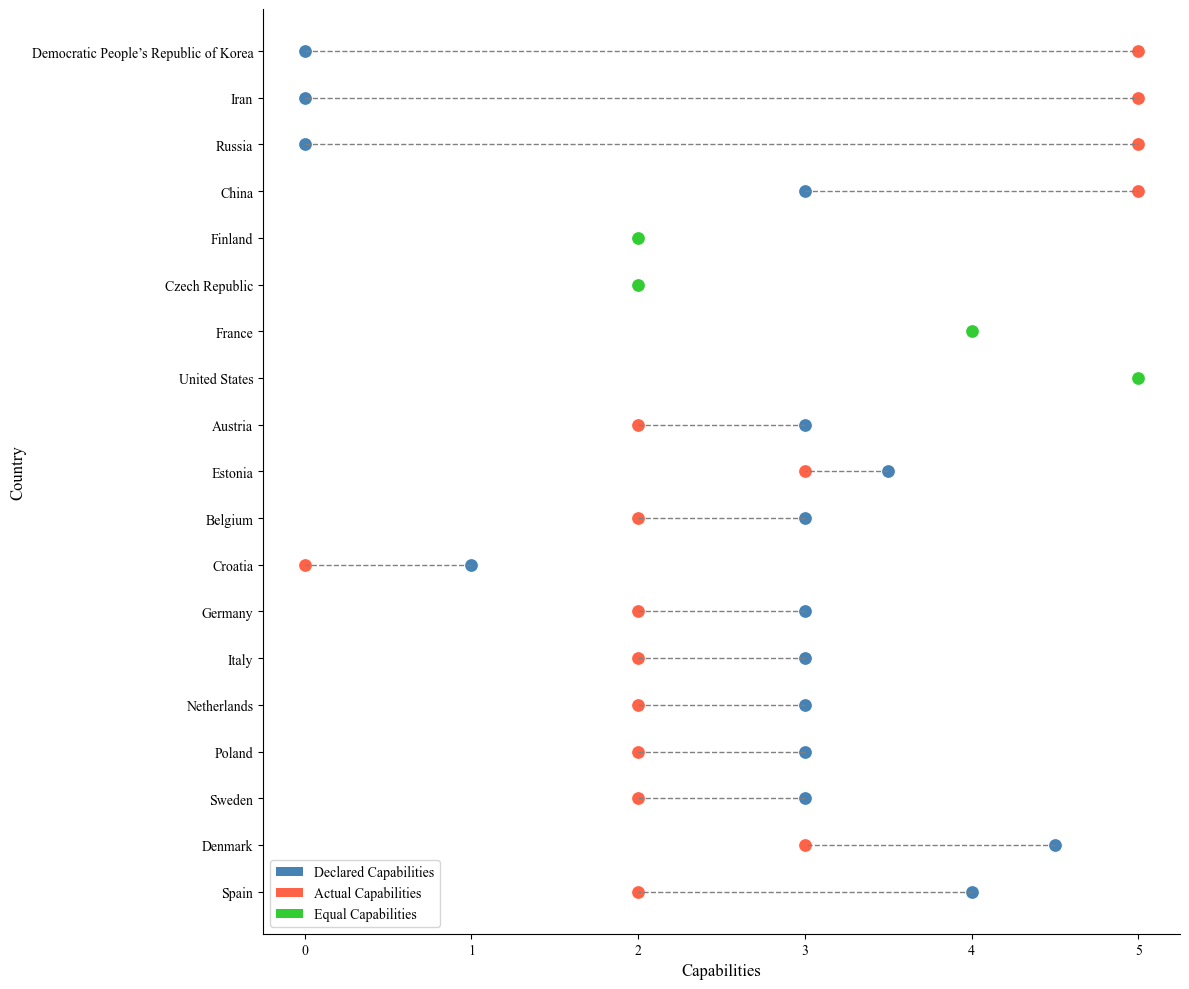
\includegraphics[width=1\textwidth]{Images/cybercap.png}
    \caption{\textit{Cyber Transparency Index \autocite[4]{faesen_2022_cyber}}}
    \label{fig:cybercap}
\end{figure}

Several analytical frameworks have been developed to assess the cyber power of a state. Each model focuses on a different approach to the power concept. In this analysis, we examine Nye’s \textit{Three Faces Model } \autocite{nye_2010_cyber}, the\textit{ Klimburg’s Power Integrated Capability Model} \autocite{klimburg_2011_cybersecurity} and the \textit{Betz and Stevens Four Dimension Model} \autocite{betz_2011_cyberspace}. All the models present power as a form of domination, in contrast to power as empowerment, \parencite{haugaard_2012_rethinking, dunncavelty_2018_europes} with the expectation of Klimburg.

According to Nye  \textcite{nye_2010_cyber}, both hard and soft power can be used to achieve political goals in cyberspace. His “Three Faces Model” identifies three types of power relations, that are not exclusively adopted only in the cyber environment between two different actors (A and B in this case). Nye identified the specific means and methods with an effect in cyberspace, which constitute power \autocite{vanhaaster_2016_assessing}). 

\begin{enumerate}

   \item The 1st face refers to the capacity of an actor (A) to force another actor (B) to engage in actions that they would not have taken otherwise. The author investigated the utilisation of malware or other attack vectors, such as DDoS attacks, to disrupt critical national services and coerce B to take measures to counter the attack. 
   \item The 2nd face involves A’s strategies to block B’s actions. Chinese “Great Firewall” is an empirical example. Nye referred to this as an agenda-setting power.
   \item The 3rd face refers to A’s power to influence B’s preferences. The author uses the example of threats to punish bloggers who disseminate censored material as preventive actions to shape their preferences.
\end{enumerate}

\begin{table}[htbp]
  \centering
  \caption{\emph{Three Faces Model of Cyberpower according to Nye \textcite{nye_2010_cyber}}}
  \begin{tabular}{p{4cm}p{4.5cm}p{5.5cm}}
    \toprule
    \textbf{Type of Power} & 
    \textbf{Hard Power} 
            (Nye) & 
    \textbf{Soft Power} 
            (EU's case) \\
    \midrule
    1st Face (A induces B to do what B would initially otherwise not do) & 
    \begin{itemize}
      \item Denial of Service attacks
      \item Insertion of malware
      \item Scada disruptions
      \item Arrests of bloggers
    \end{itemize} &
    \begin{itemize}
      \item Cybersecurity Act
      \item Mutual Defense Clause: Art. 42(7) of the TUE
      \item Cyber Diplomacy Toolbox for diplomatic retaliation
      \item NIS 1 \& 2
      \item European Cyber Defence Policy
    \end{itemize} \\
    \midrule
    2nd Face (A precludes B’s choice by the exclusion of B’s strategies) &
    \begin{itemize}
      \item Firewalls, filters, and pressure on companies to exclude some ideas
    \end{itemize} &
    \begin{itemize}
      \item Budapest Convention
      \item European Chips Act
    \end{itemize} \\
    \midrule
    3rd Face (A shapes B’s preferences so some strategies are never even considered) &
    \begin{itemize}
      \item Threats to punish bloggers who disseminated censored material
    \end{itemize} &
    \begin{itemize}
      \item General Data Protection Regulation (GDPR)
      \item AI Act
    \end{itemize} \\
    \bottomrule
  \end{tabular}
  
\raggedright
    \bigskip
    Source: Elaboration from Dunn Cavelty \textcite[11]{dunncavelty_2018_europes} (author’s example).
\end{table}



Nye’s model implies that cyber capabilities can produce both hard and soft powers \autocite[5]{nye_2010_cyber}. In this regard, the European Union, unlike Nye’s examples, does not have the hard power capabilities to achieve political objectives for each of the faces. However, EU legislation gives us the opportunity to assess EU cyper power through legislative acts, which lie more as soft power instruments rather than harder ones. Furthermore, the distinction between hard and soft cyberspace is difficult \autocite[5]{dunncavelty_2018_europes}. 

Nye suggests that cyber capacities are widespread, with all actors capable of conducting diverse cyber activities, such as denial-of-service attacks, issuing threats, controlling information, and suppressing ideas. This widespread nature casts doubt on its effectiveness as an independent analytical tool for policymakers, despite its significance in academia \autocite{vanhaaster_2016_assessing}.


\begin{table}[htbp]
  \caption{\emph{Klimburg Power Integrated Capability Model}}
  \begin{tabular}{p{7cm}p{7cm}}
    \toprule
    \textbf{Type of Power} & \textbf{Definition} \\
    \midrule
    Integrated Government Capability & Ability to deliver joint action \\
    \midrule
    Integrated Systems Capability & Ability to work through international alliances and partnerships \\
    \midrule
    Integrated National Capability & Ability to use non-state cyber elements within a country in direct support of policy \\
    \bottomrule
  \end{tabular}
  
    \raggedright
        \bigskip
    Source: Elaboration from \textcite[12]{dunncavelty_2018_europes}.
\end{table}

The Klimburg Power Integrated Capability Model understands cyber power in terms of integrated capabilities, which can shape the cybersecurity landscape \parencite{kasper_2021_the, klimburg_2011_cybersecurity}. According to \textcite{klimburg_2011_mobilising}, cyber power is the result of distributed forces. His model includes several dimensions, such as the ability to coordinate government actions, collaborate with international partners, and engage with non-state actors (both businesses and hacktivists) \parencite{dunncavelty_2018_europes, klimburg_2011_cybersecurity}. The model implies a more defensive posture of cyber power rather than an offensive character aimed at coercing other actors. The concept of cyber resilience, which has become increasingly relevant in Europe, stems from this model. As \textcite[6]{dunncavelty_2018_europes} stated, \textit{there cannot be any true cyber-power without cyber-resilience.}

A common critique is related to the EU, which according to several scholars \parencite{kasper_2021_the, klimburg_2011_cybersecurity, sliwinski_2014_moving}, does not have sufficient cyber power. This is because, by embedding the realist assumptions of state power, scholars give more importance to the 1st face or more simply to the military side of power, which creates difficulties for the EU due to the characteristics of its political project and the uncertainty in assessing cyber capabilities \autocite{dunncavelty_2018_europes}. However, the EU is more focused on cyber power based on cooperation instead of coercion because of its nature and scope, which highlights the main difference between the EU and other organisations such as NATO. 

Authors such as \textcite{kasper_2021_the} further explored the Klimburg Power Integrated Capability Model by adding a new layer that pertains to the strategic narratives of European cyber power. The authors stated that the EU has not yet been able to formulate a strategic identity narrative while opting for a non-military approach regarding its international approach to cybersecurity \autocite[64]{kasper_2021_the}. Indeed, the EU's involvement in international forums and conferences and the continuous growth of its cyber capabilities, which extend beyond securing the digital market, serve as examples of its increasing cyber power. Doubts remain regarding the hard cyber power capabilities of the union. 

The \textcite{betz_2011_cyberspace} model effectively applies \textcite{barnett_2005_power} power taxonomy to the realm of cyberspace, providing a distinct categorisation of power manifestations within this domain. This model introduces an additional layer to the Three Faces of Power model by adopting a post-structuralist approach, perceiving power as circulating within social relationships \autocite{dunncavelty_2018_europes}. 

\begin{table}[htbp]
  \centering
  \caption{\emph{Betz and Stevens (2011) Cyber Power Taxonomy}}
  \begin{tabularx}{\textwidth}{p{4cm}p{5cm}p{5cm}}
    \toprule
    \textbf{Type of Power} & \textbf{Definition} & \textbf{Examples} \\
    \midrule
    Compulsory & Coercion to change the behaviour of another actor & Control of machines or networks \\
     & Deploying non-material resources & \\
    \midrule
    Institutional & Indirect control of another actor through institutions & Influence behaviour through institutions \\
     & Norms and Standards & \\
    \midrule
    Structural & Cyberspace as a structure which can facilitate or disrupt the actors that are connected & Changing structures \\
    \midrule
    Productive & Creation of social subjects through discourse & Reproduce, construct, and reinforce narratives \\
    \bottomrule
  \end{tabularx}
  
  \raggedright
  \bigskip
  Source: Elaboration from \textcite{betz_2011_cyberspace} and \textcite{dunncavelty_2018_europes} .
\end{table}

The model identifies four distinct types of power in the cyberspace context \parencite{betz_2011_cyberspace, dunncavelty_2018_europes, vanhaaster_2016_assessing}:

\begin{enumerate}
    \item \textbf{Compulsory Power}: This type of power involves the use of coercion to compel another actor to change its behaviour. It can be exerted through the control of machines or networks, as well as through the deployment of non-material resources. For instance, a state may use cyber-attacks to disrupt the operations of an adversary or hacktivists may employ cyber means to force a corporation to change its policies.
    \item \textbf{Institutional Power}: In category, power is exercised indirectly through institutions. Actors may influence the behaviour of others through the establishment and manipulation of norms, standards, and protocols in cyberspace. Governments and international organisations, for example, can shape behaviour through the creation of cybersecurity regulations and standards that impact the actions of various actors in the digital realm.
    \item \textbf{Structural Power}: This type of power acknowledges cyberspace as a structure that can either facilitate or disrupt the actors connected to it. Actors may wield power by altering or controlling the underlying structure of cyberspace. For instance, a powerful tech company might shape the architecture of the Internet or a state might exert control over the global routing of data to enhance its strategic advantage.
    \item \textbf{Productive Power}: Productive power in cyberspace refers to the creation of social subjects through discourse. This involves shaping and influencing narratives, constructing ideologies, and reinforcing certain beliefs and values in the digital space. Governments, media organisations, and influential online communities may engage in shaping public opinion and generating narratives that support their interests.
\end{enumerate}

Conversely, the Klimburg and Nye models suggest that cyber capabilities can be utilised within a specific domain or context. Alternatively, Betz and Stevens adopted a post-structuralist perspective on cyber power \autocite{dunncavelty_2018_europes}, emphasising the location of the conflict rather than solely on the cyber capabilities deployed \autocite{vanhaaster_2016_assessing}. All cyber tools have the potential to be employed to achieve various state objectives, whether they are related to military, political, or economic power. \textcite[21]{vanhaaster_2016_assessing} argues that \textit{it is impossible to create a comprehensive overview of cyber power distribution, as it relies on all dimensions of power}. Because these dimensions are contextual and some are temporary, the field should refrain from adopting a universal model for assessing cyber power and instead employ frameworks on a case-by-case basis. 

In conclusion, \textcite{vanhaaster_2016_assessing} builds a cyber capacity framework on the state’s instruments of power as described by various authors and frameworks, namely Carr, Mann, and DIME(FIL) proponents.  These scholars have expounded on how these instruments can be effectively employed to exert influence in traditional domains such as land, sea, and air. The model in question seeks to expand this discussion into the realm of cyberspace and identify the cyber analogues of these instruments of state power. This endeavour holds significant importance given the prevailing cyber power discourse's tendency to predominantly focus on the means aspect of power, such as the capacity for conducting \textit{Distributed Denial of Service} (DDoS) attacks and the allocation of budgets for acquiring malware. Nevertheless, this viewpoint falls short of encompassing a myriad of factors that collectively contribute to a state's capacity to achieve its objectives in cyberspace. This study presents a more comprehensive and holistic approach to analysing cyber power by identifying and understanding the cyber equivalents of traditional instruments of state power. This inclusive approach incorporates consideration of factors such as the extent of influence, the specific domain of operation, the magnitude of impact, associated costs, and the means employed, each of which plays a vital role in comprehending a state's true capability to wield power in the digital arena. 

\begin{table}[htbp]
  \centering
  \caption{\emph{State's Power Instruments and Cyber Capacities according to \textcite{vanhaaster_2016_assessing}}}
  \begin{tabularx}{\textwidth}{p{2.5cm}X}
    \toprule
    \textbf{Instrument} & \textbf{Cyber Capacities} \\
    \midrule
    \multirow{2}{*}{Political} & Coordination \\
    & Cyber-capacities to be used abroad \\
    & Deterrence \\
    \midrule
    \multirow{2}{*}{Informational} & Manipulation of information \\
    & Legitimization through social media \\
    & Intelligence gathering \\
    \midrule
    \multirow{2}{*}{Economical} & Protect own industries \\
    & Secure infrastructure \\
    \midrule
    \multirow{2}{*}{Military} & Kinetic-Cyber coordination \\
    & Military infrastructure control \\
    \midrule
    Other & Influence institutions \\
    & Arrests or prosecuting \\
    & International Law applied to cyber \\
    \bottomrule
  \end{tabularx}
  \label{tab:state-power-cyber}
\end{table}


\newpage

The framework serves as a foundational point for analysing cyber strategies, considering five essential dimensions that warrant a thorough case-by-case assessment:
\begin{itemize}
 \item \textbf{Scope}: This dimension encompasses the extent of cyber power, the number of actors involved, and the geographic area covered.
 \item \textbf{Domain}: Here, the focus lies on the specific areas or sectors where cyber power is wielded, be it in the military, economic, or political domains.
 \item \textbf{Weight}: This dimension evaluates the relative importance or significance of cyber power in comparison with other forms of power at play.
 \item \textbf{Costs}: The resources necessary to develop and sustain cyber power are scrutinized by incorporating financial, human, and technological resources.
 \item \textbf{Means}: Finally, attention is paid to the specific tools, techniques, and capabilities employed to exercise and manifest cyber power.
\end{itemize}

Considering these five dimensions, the framework provides a comprehensive and multifaceted approach to the analysis of cyber power strategies, thereby offering valuable insights into the dynamics and effectiveness of such endeavours. This framework will be applied in the analysis of the cyber realm of the War in Ukraine to retrieve key lessons for other actors. 



\chapter{Cyber Defense Matters}

\section{Exploratory Data Analysis of Cyberattacks}

In this chapter, an exploratory data analysis will be executed on cyber operations data from different sources, tracing trends, differences and insights that can be useful for the purpose of this research. One approach to assess the cyber defense strategies of the European Union members is to understand how those countries counter the attacks. Furthermore, it will help to recognise if the war in Ukraine had a direct effect on cyber operations in EU countries. 

\begin{figure}[H]
    \centering
    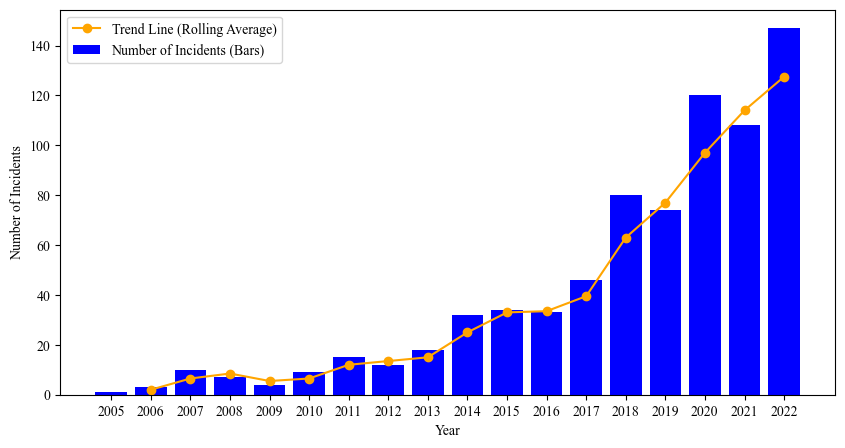
\includegraphics[width=1\textwidth]{Images/total_cyber.png}
    \caption{\textit{Total Cyber Operations from 2005 to 2022}}
    \source{Source: Cyber Operations Tracker}
    \label{total_cyber.png}
\end{figure}

As expected, in Figure \ref{total_cyber.png} the total number of cyber operations is constantly increasing. Noticeably, during the COVID-19 pandemic, we have experienced an increase of about 62.16\% of attacks compared to 2019. The surge in cyberattacks can be attributed significantly to the widespread adoption of remote work. This increase is primarily because individuals working from home lack the same level of inherent security and deterrent measures present in traditional office environments \parencite{nabe_2020_impact}. 

\begin{figure}[H]
    \centering
    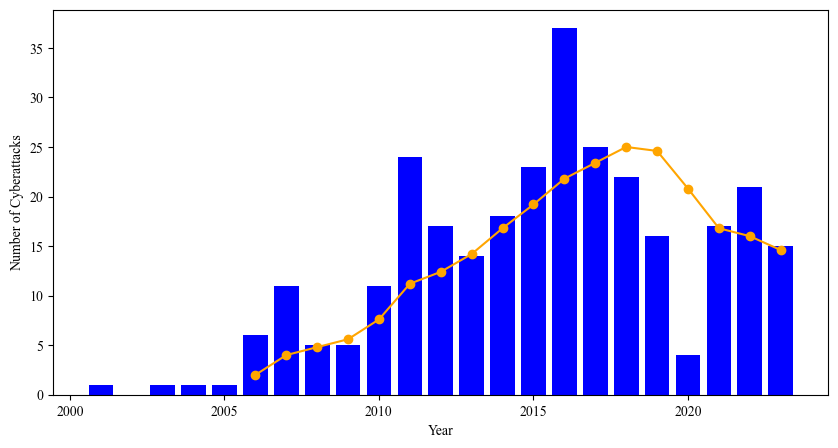
\includegraphics[width=1\textwidth]{Images/total_cyber_EU.png}
    \caption{\textit{Total Cyber Operations from 2000 to nowadays}}
    \source{Source: EuRepoC}
    \label{total_cyber_EU.png}
\end{figure}


However, it is important to note that the European context exhibits a decrease in recorded cyberattacks during the COVID-19 pandemic. These findings, as elucidated by the insights provided by Kerstin Zettl-Schabath, on behalf of the EuRepoC coding team, can be attributed to several factors. EuRepoC's approach to data collection differs from that of the Cyber Operations Tracker, which primarily focuses on politically motivated cyber incidents. According to Kerstin Zettl-Schabath \footnote{Kerstin Zettl-Schabath is part of the Coding Team of EuRepoC. The information was obtained through an exchange of emails.}, EuRepoC does not count non-politically motivated and fully disclosed cyberattacks in its database. Therefore, while it is true that overall cyberattacks increased during the pandemic, many of these attacks were more economically motivated and not necessarily politically driven. This fact underscores the importance of considering the motive and nature of cyber incidents when analysing the data.

Kerstin Zettl-Schabath provides several potential explanations for the discrepancy between EuRepoC's data and other sources:
\begin{enumerate}
    \item EuRepoC places particular emphasis on confirmed CIA (Confidentiality, Integrity, Availability) violations in their data collection. Some incidents recorded by other sources may be considered as \textit{attempted attacks} without confirmed CIA violations, leading to differences in reported incidents. It is essential to consider the criteria used by each database for assessing the intensity and impact of cyber incidents.
    \item EuRepoC's inclusion criteria do not cover genuine cybercrime cases that lack political or state involvement. This criterion was only added to their codebook in recent years. The rapid increase in non-politicized cybercrime incidents throughout the first year of the COVID-19 pandemic could account for part of the explanation for the lower incident count in EuRepoC's database compared to sources with different inclusion criteria.
    \item The assignment of incidents to a specific year can vary between databases based on criteria such as the actual start of the operation. This discrepancy may lead to differences in the reported number of incidents in a given year.
    \item Kerstin Zettl-Schabath also suggests a theoretical explanation related to the diversion of resources and capacities during the COVID-19 pandemic. The pandemic may have absorbed more resources at the state cyber level, leading to both fewer offensive cyber actions and fewer detections and attributions of incidents, which would have been relevant to EuRepoC's politically connoted inclusion criteria
\end{enumerate}

\begin{figure}[H]
    \centering
    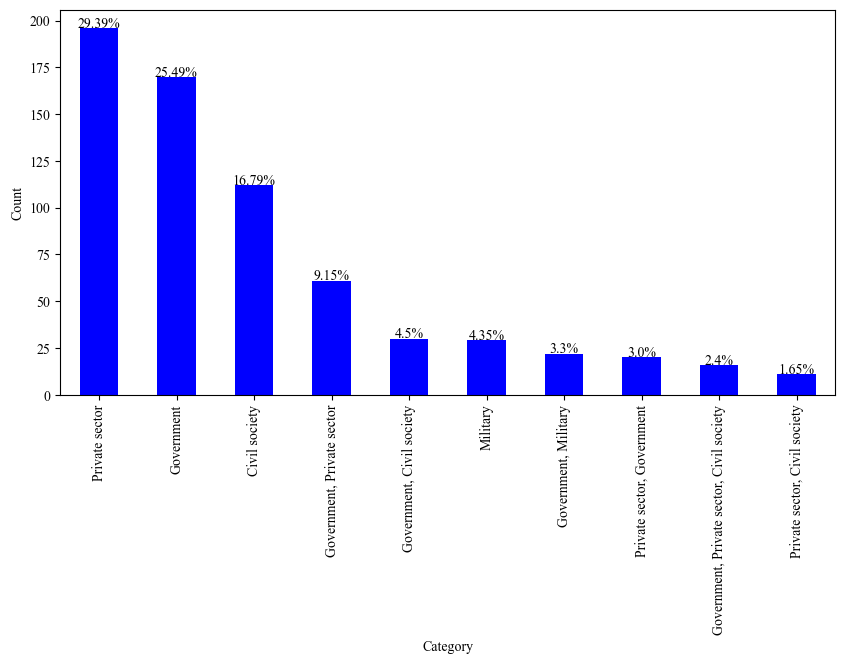
\includegraphics[width=\textwidth]{Images/top10sect.png}
    \caption{Top 10 Sectors Affected by Cyber Operations}
    \source{Source: Cyber Operations Tracker}
    \label{fig:top10sect}
\end{figure}

The categories most attacked are the private sector (29.35\%) and the government (25.22\%), while the military category constitutes 4.42\% of the worldwide cyber operations from 2005. Differently from the government and private sector, attacks on the military IT infrastructure are less disclosed while being at the same time difficult to be successful to its increase securitization. 

\begin{figure}[H]
    \centering
    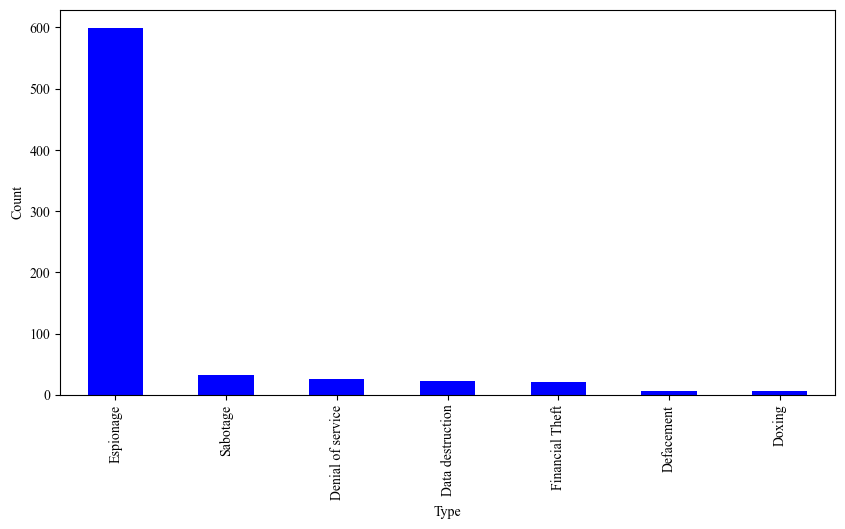
\includegraphics[width=\textwidth]{Images/top10type.png}
    \caption{Methods to conduct Cyber Operations}
    \source{Source: Cyber Operations Tracker}
    \label{fig:top10type}
\end{figure}

For what regards the goal of attacks, mainly relates to espionage. Cyber adversaries often seek to infiltrate both private sector and government networks to gather sensitive information, proprietary data, or state secrets. Espionage attacks aim to gain unauthorized access to critical data for intelligence purposes, economic advantage, or strategic planning. These attacks can have far-reaching consequences, ranging from compromising individual privacy to jeopardizing national security. 

\section{Why no destructive cyberattacks? }

Destruction-focused cyberattacks are relatively less common for several significant reasons. Firstly, these attacks often leave a more traceable trail of evidence, making it easier for cybersecurity experts to identify and attribute the source of the attack. Additionally, destructive cyberattacks can escalate conflicts and lead to severe real-world consequences, deterring some threat actors. Technical complexity and the need for deep knowledge of target vulnerabilities also make such attacks less attractive compared to data theft. Moreover, many cyberattacks are politically or strategically motivated, aiming to influence public opinion or cause economic disruption rather than physical destruction. International norms discourage destructive cyber operations and the cost-benefit analysis that cybercriminals and state-sponsored actors perform further contribute to their relative infrequency. While destructive cyberattacks are not unheard of, their risks and consequences make them a less common choice in the cyber threat landscape. 

On the other hand, for what regards the European context, the motive behind the attacks is mostly unknown. This is because cyberattacks are a major of the time part of operations that includes cyber, information and influence sphere with political objectives that are not specified with a blurred portrait as hybrid operations do. The EuRepoC use the codification from the Conflict Issues by the Conflict Barometer of the Heidelberg Institute for International Conflict Research (HIIK), to identify several cyber-conflict issues. 35\% of the issues relate to the system/ideology and international power conflicts. The first refers to change and/or influence in internal aspects of state affairs (socio-economic, legal, or political orientation). International power relates to changes in the relations of power in the international system or one of its regional systems \parencite{hiik_methodology}.

\begin{figure}[H]
    \centering
    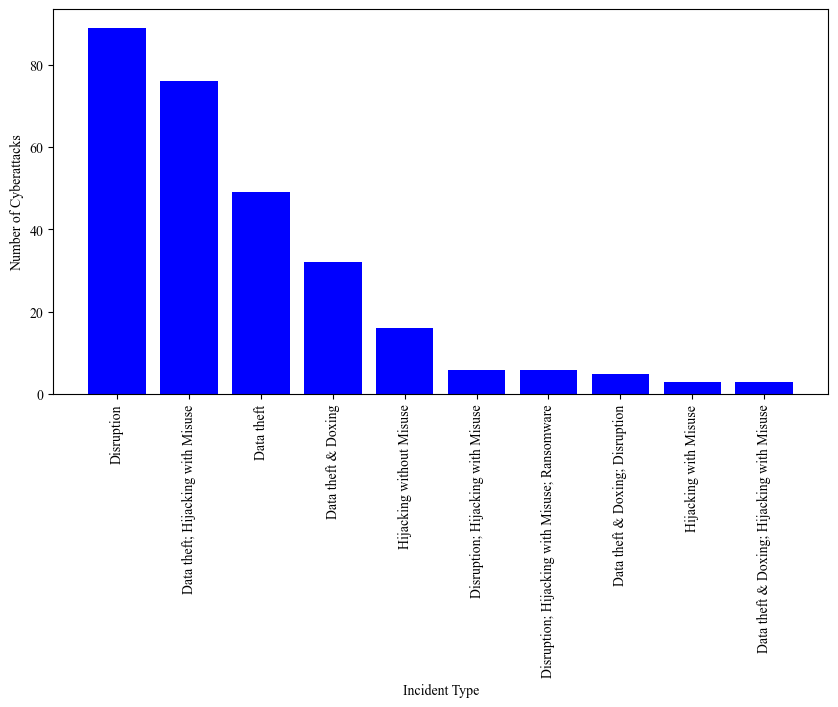
\includegraphics[width=\textwidth]{Images/eu_type.png}
    \caption{Classification of Cyber Operation in the EU by type}
    \source{Source:EuRepoC}
    \label{fig:eu_type}
\end{figure}

From 2001 to nowadays, the principal attack vectors for each of the modalities have evolved significantly. In the realm of disruption, attackers have increasingly employed distributed denial of service (DDoS) attacks, ransomware, and malware to disrupt critical systems and services. Meanwhile, in the domain of data theft, attackers have leveraged techniques such as phishing, social engineering, and advanced persistent threats (APTs) to gain unauthorized access to sensitive information and steal data. 

\section{Intensity of Cyber Operations}

The European countries have only in recent years given strategic importance to cyberspace and its security. Overall, the European countries were not able to handle the cyberattacks to avoid the disruptions, as Figure \ref{fig:avg} suggests. Firstly, there is a lack of sufficient infrastructure and investment to support the cybersecurity and cyber-defense policies and institutions in Europe \autocite{petratos_2014_cybersecurity}.  Additionally, the flexible and modern network technologies used by business organizations have opened the door for cybercriminals to initiate cyberattacks, leading to disruptions in the business process \autocite{sudar_2020_analysis}). The European Union also faces limitations as a cybersecurity actor, including its intergovernmental character and the lack of a collective vision on cyber-security among member states \autocite{sliwinski_2014_moving}


\begin{figure}[H]
    \centering
    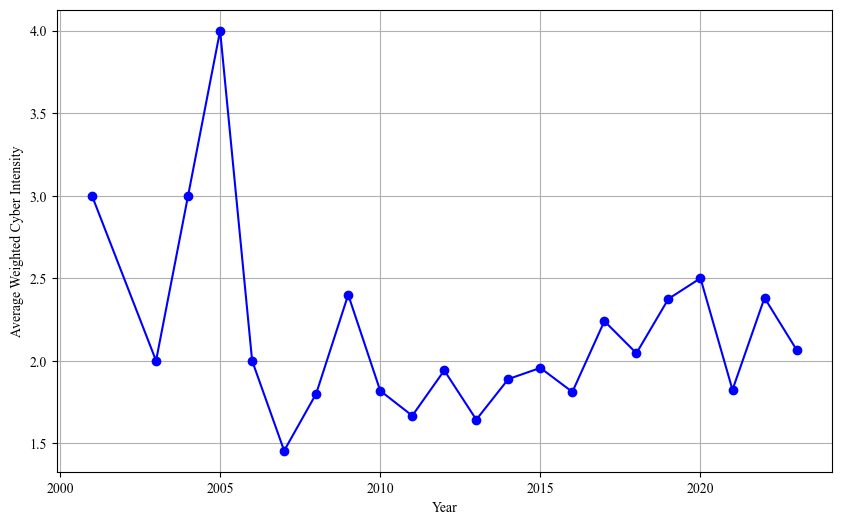
\includegraphics[width=\textwidth]{Images/avg.png}
    \caption{Average Weighted Cyber Intensity per Year in EU Countries}
    \source{Source:EuRepoC}
    \label{fig:avg}
\end{figure}

For many different cyber incidents, the average cyber intensity has mostly remained low. Even in the case of the Estonia 2007 cyberattacks, where the EuRepoC acknowledged that the level of disruption was less severe than initially predicted, this pattern persisted. But it's important to remember that this incident still has political ramifications since it had a major influence on how NATO and the European Union would respond to state-sponsored cyberattacks.

On the other hand, some specific cyber incidents have displayed a noticeably high level of cyber intensity, such as the Ransomware House attack on the Hospital Clinic de Barcelona. Such incidents come into the high-intensity category, with a grade of 6 on the intensity scale, and are defined by their major interruption, probable data theft, system hijacking, and significant spatial and temporal consequences. The attack on Hospital Clinic de Barcelona serves as a sobering reminder of the changing and more advanced cyber risks critical infrastructure must contend with, particularly in the healthcare industry, where the stakes are very high.  

While the highest average in 2005 is associated with Poseidon, often referred to as the \textit{Poseidon Group}, which is a cyber espionage group known for its advanced and targeted attacks. Its activities primarily revolve around conducting cyber espionage campaigns against specific targets, with a particular focus on governmental and diplomatic entities, as well as critical infrastructure organizations. It was disclosed by Kaspersky in 2015 and has affected France, Russia, Brazil and United Stated among other countries\footnote{For more information: https://securelist.com/poseidon-group-a-targeted-attack-boutique-specializing-in-global-cyber-espionage/73673/}.

%%% Section about statistics of War in Ukraine %%% 


\chapter{Cyber Realm of War in Ukraine}

The conflict in Ukraine had a significant impact on international relations. This study seeks to examine the patterns and trends observed in the cyber aspect of the Ukrainian conflict, specifically focusing on the defining characteristics of the cyber realm within this context. Furthermore, it aims to evaluate the strategic efficacy of the cyber operations employed during the war between Ukraine and Russia.  By leveraging these resources, this research aims to offer a comprehensive analysis of the cyber dimension of the Ukrainian conflict, fostering a deeper understanding of its implications. This chapter critically examines the failure of Russian cyber operations in Ukraine by analysing significant cyber events that occurred during wartime, assessing the accountability of Russian cyber troops, and evaluating the extent of Western assistance. The outcome of this analysis will show the main characteristics of cyber operations in wartime, which will be searched on the European cyber strategies further in this work.

The hypothesis behind this study rests on the Russian failure in its cyber operations in Ukraine, not only due to the Western assistance, which has been widely discussed in the literature but also because of the inefficiency in the preparation and execution of military and cybernetic plans. While we have evidence of the kinetic side failure, the same cannot be said for cyberspace. In this regard, the work aims to develop further this topic.

The cyber dimension of the war in Ukraine has garnered significant attention and interest among researchers and analysts. Numerous studies have delved into the intricate patterns and evolving trends of cyber-attacks, assessing the strategic effectiveness of cyber operations, and contemplating broader implications for future conflicts. Companies directly involved, such as Microsoft and Google, have progressively developed analyses of Ukrainian cyberspace, presenting the main Russian cyber operations and how they support cyber defence.

Additionally, the research work will employ insightful research from the Carnegie Endowment for International Peace collection on cyber conflict in the Russia-Ukraine War. These studies explore cyber events chronologically, providing strategic significance \parencite{levite_2023_integrating, lewis_2022_cyber}, while others focus on the structural problems of inter-institutional cooperation within the Russian agency regarding cyber operations \autocite{wilde_2022_cyber}. The literature agrees with defining the war outcomes, both from the cyber and kinetic perspectives, as a failure of the Russian Federation. However, there were differences in the key factors that led to this outcome.

According to \textcite{lin_2022_russian}, Russian cyber failure relies on the unpredictability of cyber operations, which has caused Russian military command to avoid their strategic use, instead of relying on hard military power. Moreover, scholars agree that Western assistance has strongly influenced Ukraine's cyber defence in various ways. \textcite{beecroft_2022_evaluating} qualitatively analysed how the West helped Ukraine build a more resilient defence.

Finally, this chapter will rely on CyberPeace Institute Quarterly research, a highly reputable NGO specializing in cyber politics, to avoid political bias that may be present in such a theme. The latter provides us with the opportunity to explore data on cyber operations from both sides of the conflict, with a focus on human rights.

\section{Exploring the Cyber Dimension of the Russian Invasion of Ukraine}

On February 24, 2022, the events had a profound and lasting impact on international relations. The visual portrayal of bombings in Ukrainian cities served as a stark reminder, while the consequential political and economic effects reverberated globally. Simultaneously, as Russian Main Battle Tanks (MBTs) and Armoured Personnel Carriers (APCs) breached the Ukrainian border, the cyber domain played an integral role in both laying the groundwork and disrupting the adversary. Despite facing a significantly more powerful opponent in the Russian military, Ukraine showed remarkable resilience, not only withstanding the onslaught but also mounting counteroffensives that decisively shifted the balance of power on the battlefield.

\subsection{Overview between Russian cyberattackers and Ukraine cyber defenders}
Before starting our discussion, it is crucial to identify the relationship between Russian cyber and kinetic forces, especially by emphasizing the inter-institutional relationships between different realities. Comparing them to the Ukraine counterpart is also beneficial to the discussion, to have an overview of forces that were (and are) in the cyber field.  

\textbf{Russia Cyber Structure}

The first main difference between Western and Russian cyber-attitudes relies on the term used to identify those actions in the cybernetic environment. Russians do not use the term cyber; instead, they refer to the information (\textit{informatsiya}) confrontation in the political and military lexicon to describe the range of operations—both technical and psychological, code, and content—that can be deployed against adversarial systems and decision-making \autocite[3]{wilde_2022_cyber}. This perspective is prevalent in Russia, and can be traced back to the Soviet era. It significantly influences not only the methodologies employed by Russia, but also the objectives pursued through its global-scale information operations. Offensive cyber operations constitute a specific subset of operations that seek to influence the information environment. These are integral components of a broader spectrum of operations that share the common objective of influencing the environment. For the purposes of our research, we adopt the term cyber to encompass all operations aimed at exerting influence on the information environment through the use of computer networks and electronic systems.

\begin{figure}[H]
\centering
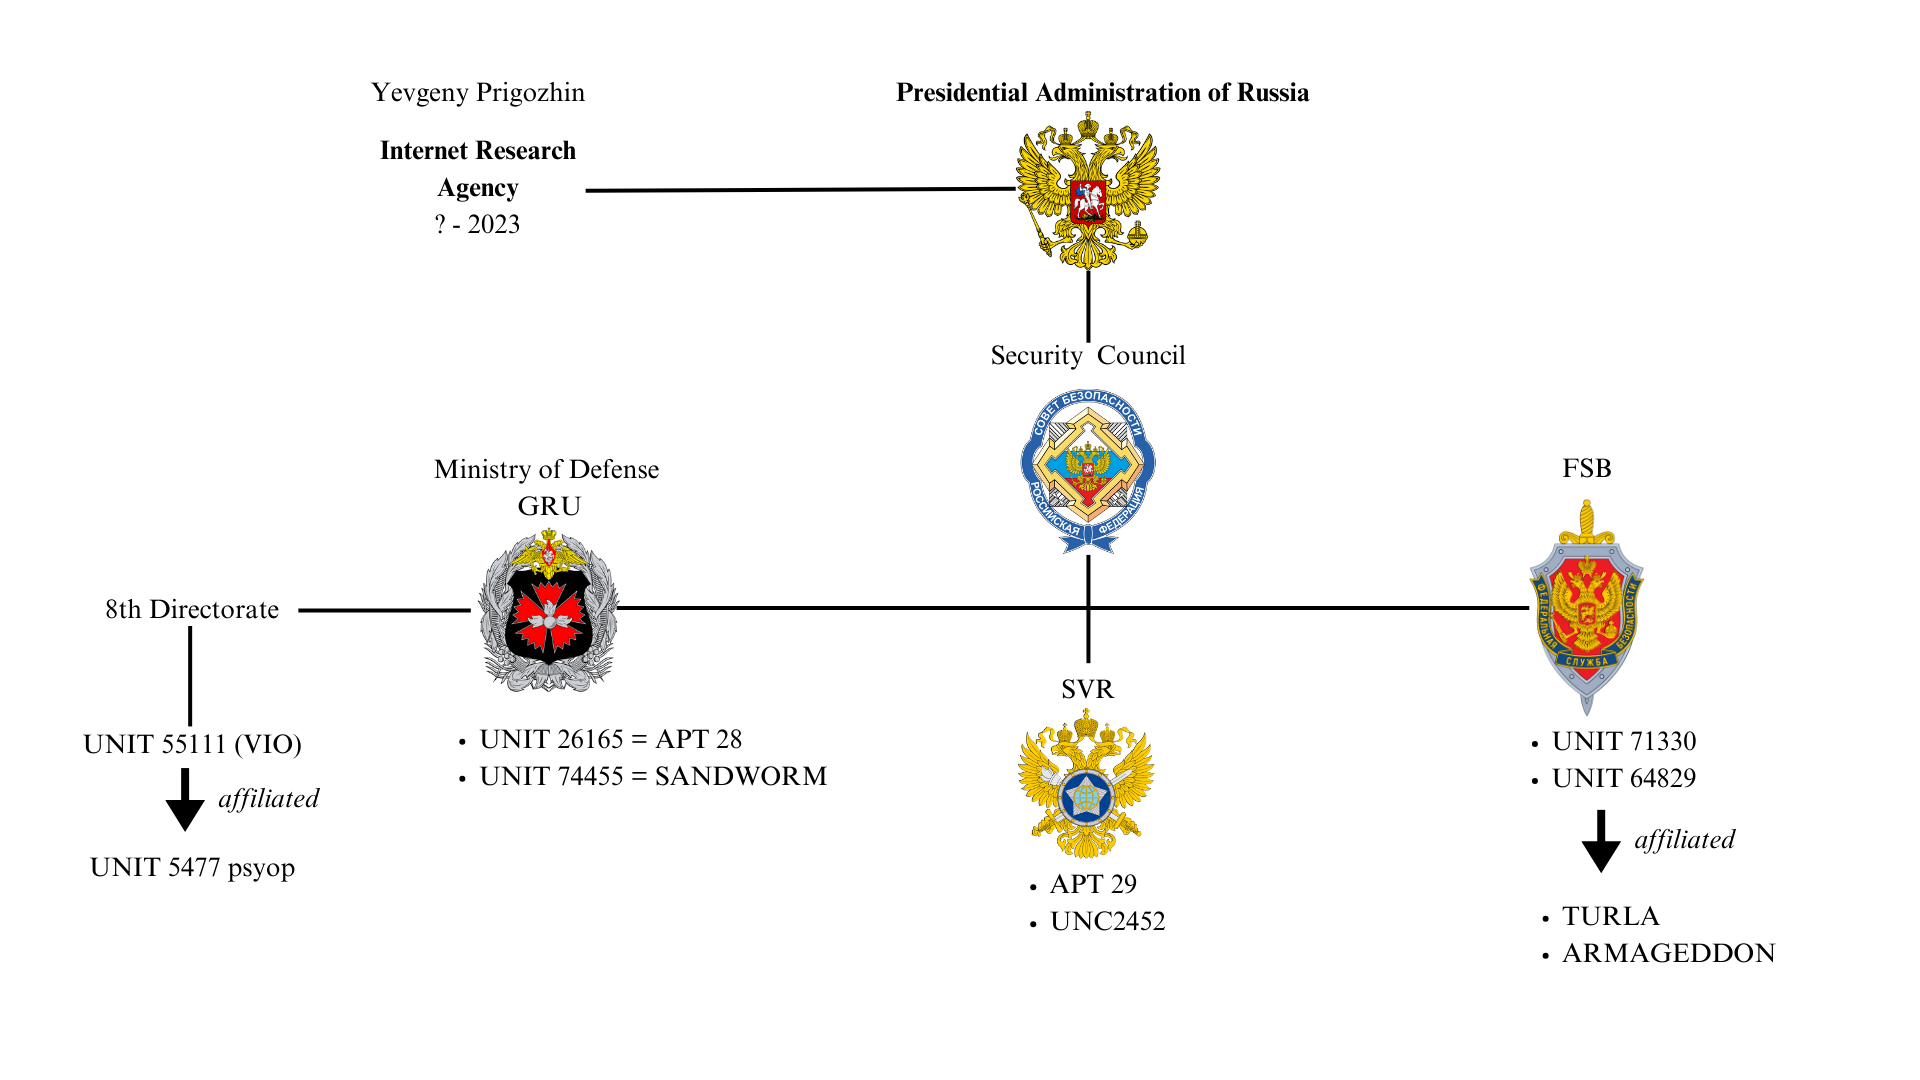
\includegraphics[width=1\textwidth]{Images/RussiaCyber.png}
\caption{\textit{Russia Cyber Structure. Author's representation from \textcite{wilde_2022_cyber} and Mandiant}}
\label{RussiaCyber.png}
\end{figure}

Historically, the information environment was under the exclusive control of security agencies in the Soviet Union, such as the KGB. As a result, modern Russian bureaucracy continues to adhere to the principles established by Soviet \textit{nomenklatura}, even in the realm of cyber operations. In recent times, Western intelligence communities, in cooperation with threat intelligence companies such as Mandiant and Recorded Future have tried to link Russian threat actors with their bureau, in order to understand their task as state-sponsored threat actors. 

Most Russian operations are conducted by \textit{Glavnoye Razvedyvatelnoye Upravlenie} (GRU), the foreign military intelligence agency of the Russian Federation, specifically through Unit 54777. This unit is part of a larger institutional organization known as \textit{Voyska Informatsionnykh Operatsiy} (VIO), or Information Operations Troops. The actions of the Russian cyber apparatus are directly supervised and guided by the Security Council, exemplifying political control over military mechanisms \autocite{wilde_2022_cyber}. The literature offers numerous examples of how Unit 54777 operated during peacetime, exerting influence over political scenarios (e.g., Georgia 2008), disrupting critical services (e.g., Estonia 2007), and attempting to influence electoral processes (e.g., United States 2016). Unit 54777 specialised in psychological operations, considered the feature with the most impact on the Russian cyber strategy \autocite{wilde_2022_cyber}.

Official cyber units that are embedded with the Russian military organisation are hardly recognized for their methods of attack. For this reason, threat intelligence services categorise Russian threat actors with code-names to simplify the clustering, while attempting to link with the Russian military structure. For instance, the Foreign Intelligence Service known as SVR (\textit{Služba Vnešnej Razvedki}) have several groups affiliated, as the APT29 is often mentioned as \textit{Cozy Bear} or the GRU Unit 745455 mentioned as \textit{Sandworm}. Mentioning the names and code-names of Russian cyber units and threat actors is important for several reasons, ranging from technical attribution to political implications. Technical attribution is established by comprehending the tactics, techniques, and procedures (TTPs) employed in cyberattacks. On the other hand, the political response involves public condemnation and establishing the link between the threat actor and their affiliated unit, often leading to sanctions imposed by the victim.

\textbf{Ukraine Cyber Structure}

Ukraine's cyber-structure has been less researched than its Russian counterpart, for obvious reasons. Since the Donbas crisis and the Russian annexation of Crimea in 2014, Ukraine has been constantly under target by Russian-led cyber operations. In 2016, Ukraine approved its first cybersecurity strategy, which acknowledged that the country's cyber infrastructure had been attacked and emphasized the need for a formal cybersecurity system. This system was designed to counter cyberterrorism and protect critical infrastructures, including the military, energy, transportation, and banking sectors. The strategy also proposed that the state would work with NATO and EU members to establish best practices \autocite{brantly_2019_cybersecurity}.

The structure of cybersecurity in Ukraine is primarily centralized and falls under the National Security and Defence Council (NSDC). The NSDC encompasses the Ministry of Defence (MoD), the Security Service of Ukraine (SBU), Ministry of Internal Affairs (MIA), the Main Directorate of Intelligence, and the State Service of Special Communications and Information Protection of Ukraine (SSSCIP). The structure, as will be discussed in the following sections, as been relatively proactive in cooperating with other intelligence agencies and private companies that have offered their know-how to support Ukraine's defence against Russian invasion. 

After the Russian invasion, the Ministry for Digitalization called for the establishment of the IT Army of Ukraine, in which every person has the possibility to contribute to disruptive attacks (such as DDoS) from their own device and network on specific targets (like Russian websites and networks). It was the first time that a government called for collective action against cyberattacks, simplifying the methods \footnote{By joining a telegram channel and downloading the script, the user could start the attack with one click.} with the aim of collecting fire powers for their objectives. 

\begin{figure}[H]
\centering
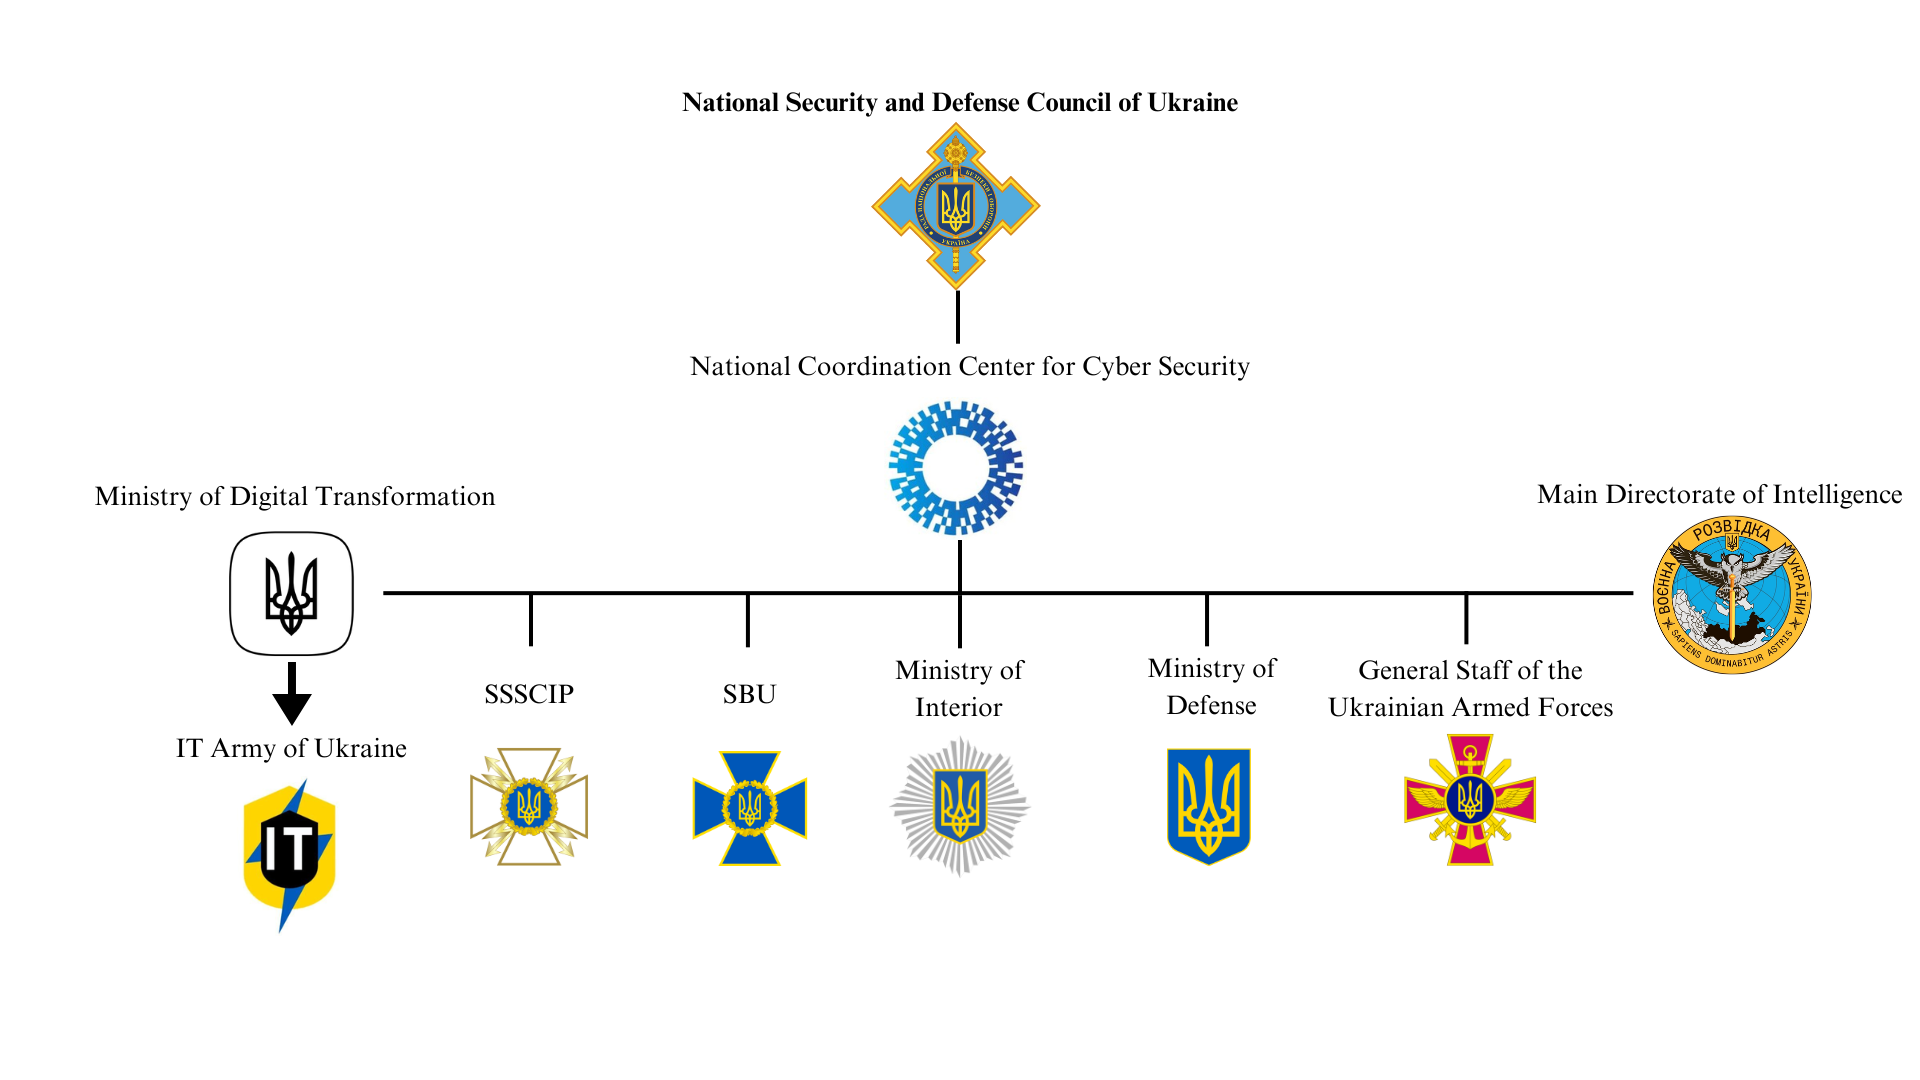
\includegraphics[width=1\textwidth]{Images/UkraineCyber.png}
\caption{\textit{Ukraine Cyber Structure. Author's representation from \textcite{brantly_2019_cybersecurity}}}
\label{UkraineCyber.png}
\end{figure}

\section{Examples of Russian Cyber Operations in Ukraine}

Tensions between Russia and Ukraine emerged prior to the 24th of February, manifested through the Crimean annexation and the Donbas conflict. Even after more than a year of fighting, the Russian Federation was unable to succeed in toppling the Kyiv government. This protracted conflict exposed the military challenges and setbacks faced by Russian forces, reminiscent of their experiences in the Chechen wars. Similarly, the outcomes of cyber operations mirrored those of kinetic military actions. Russian cyber offensives, as documented by \textcite{baetman_2022_russias}, did not yield a significant strategic impact on the overall course of the war.

On the day preceding the outbreak of the war, Russia conducted a disabling attack on Viasat's European satellite network. This targeted assault resulted in the disruption of Internet services for numerous Viasat customers in Ukraine, leading to communication breakdowns across various government agencies and businesses \autocite{willett_2022_the}. This attack stands out as a significant accomplishment of Russian forces in the realm of cyberspace. Dmitri Alperovitch\footnote{ Dmitri Mikhailovich Alperovitch is an American think-tank founder, investor, philanthropist, podcast host and former computer security industry executive.} referred to it as the most strategically impactful cyber operation in the history of wartime \autocite{baetman_2022_russias}. However, achieving effective coordination between cyberweapons and kinetic weapons poses considerable challenges. The limited strategic impact of the cyber dimension compared to its kinetic counterpart can be attributed to the integration of both domains within a combined arms approach \autocite{wilde_2022_cyber}. The Russian Voyska Informatsionnykh Operatsiy (VIO) lacked prior experience and empirical preparation for conducting destructive cyber operations during wartime. Bureaucratic obstacles have hindered efficient cooperation between agencies and the military, impeding their effectiveness in the cyber domain.

Military operations in Ukraine underwent significant changes compared to the initial expectations of a swift campaign aimed at overthrowing the Kyiv government, similar to the annexation of Crimea in 2014. However, due to Ukraine's exceptional defence capabilities and support from Western nations, the war's outcome shifted, transforming it into a war of attrition. In this attrition-based conflict, offensive cyber operations proved less suitable. The nature of cyber-attacks requires meticulous preparation and intelligence gathering, which cannot keep up with the fast-paced nature of kinetic military operations during wartime \autocite{beecroft_2022_evaluating}.

Notably, these difficulties have been empirically verified through an analysis of cyber targeting in Ukraine. Russia has predominantly utilized cyber firepower to target Ukraine's critical infrastructure. During the initial weeks of the war, Russia employed Industroyer2 malware to target the management system of the electricity grid, although no power outages occurred \textcite{willett_2022_the}. Between January 2022 and March 2023, the CyberPeace Institute documented 360 cyber incidents targeting entities in Ukraine \autocite[3a]{cyberpeaceinstitute_2023_cyber}. Microsoft, a significant contributor to Ukraine's cyber defence, stated that most destructive cyberattacks had been successfully repelled, resulting in no critical disruptions for either civilian or military sectors, except for the Viasat hack \autocite{smith_2022_defending}. However, a potential correlation between cyberattacks and kinetic attacks is worth noting. On March 4, a GRU-affiliated cyber group targeted the Vinnystia government network, followed by cruise missile strikes on March 6 and 16, targeting the Vinnystia airport and TV tower, respectively \autocite[8]{smith_2022_defending}. According to Bateman, these cyberattacks do not seem to cause any disabling effects, rendering them unsuccessful. If they were coordinated with physical attacks, they either failed to achieve the intended effects or were conducted as cyber intelligence operations in support of kinetic targeting \autocite[9]{baetman_2022_russias}. It is plausible to hypothesize that kinetic operations in Ukraine were deployed as an independent instrument aimed at tactical objectives, rather than serving as a complementary strategy to cyber operations. Another example of the cyber-kinetic paradigm can be observed on March 1, when the Russian military publicly declared its intention to destroy information-based targets in Ukraine, followed shortly by a missile strike on a TV tower in Kyiv. It is noteworthy that prior to this incident, Microsoft alerted Ukrainian authorities about a failed destructive cyberattack targeting a prominent broadcasting company \parencite{baetman_2022_russias, smith_2022_defending}. Microsoft stated that computer network operators and physical forces independently pursued a common set of priorities \autocite{microsoft_2022_an}. Although assessing the effectiveness of integrated cyber-kinetic attacks is challenging, some scholars have attempted to analyse them through case studies and assess their tactical, operational, and strategic outcomes. For example, Bateman analysed the Dnipro cyber and kinetic attacks on March 11. Although the Russian forces achieved permanent deletion of government agency data at the tactical level, the delay in emergency response to missile strikes had only marginal operational benefits. Furthermore, the strategic objective of a ground assault is neither achievable nor attempted \autocite[11]{baetman_2022_russias}.

The literature has produced several details because Russian cyber fires did not have a strategic role in the Ukraine War. Building upon the prevailing scholarly perspectives, this study contributes an additional explanation to further explore this phenomenon.

\section{Intelligence gathering rather than destruction}

Scholars concur that Russian cyber assets are primarily employed for intelligence gathering \parencite{baetman_2022_russias, levite_2023_integrating, beecroft_2022_evaluating, lin_2022_russian}. Assessing the pre-war cyber intelligence gathering activities of Russia presents inherent challenges; nevertheless, it can be argued that the strategic failure of the special military operation was significantly impacted by Russian agencies' underestimation of Ukraine's political and military capabilities. Moreover, criticism has been directed towards Russian intelligence agencies for their unreliable human sources within Ukraine, instances of financial misappropriation, historical deficiencies in analytic proficiency, and pervasive inter-service rivalries, all of which have contributed to a compromised operational environment \autocite{baetman_2022_russias}. There could be two hypotheses as to why cyberintelligence gathering was preferred over destructive gathering. First, Russian cyber forces are trained to operate during peacetime, favouring intelligence gathering over the destruction of information. As assessed previously for infrastructure targeting, it is possible that kinetic instruments were used when destructive cyber operations failed, preferring to use intelligence to better calibrate kinetic actions. However, this does not exclude the capacity of Russian forces to execute destructive cyber-attacks, as seen in NotPetya. Scholars such as \textcite{lin_2022_russian} and \textcite{levite_2023_integrating} affirmed that Russia was restrained in using its top-tier cyber assets to avoid spillover and retaliation from Western countries. They also believe that Russia may be maintaining its full cyber capacity under the shadows for future confrontations with NATO. These theses could be misleading because Russia has used its best kinetic military assets in Ukraine and showed their fallibility (several exemplars of T-90 destroyed, Kinzhal supersonic missiles intercepted, BMPT Terminator destroyed\footnote{Full list of Russian losses documented with video and photo can be found on the Oryxs website: https://www.oryxspioenkop.com/2022/02/attack-on-europe-documenting-equipment.html}).

Achieving a Cyber Pearl Harbor during wartime is not just a matter of coordination with the kinetic side, but rather a complex issue that relates to assets that are far away from being ready. For instance, during the DEFCON 2015 \textcite{krotofil_2015_rocking} presented a case study on attacking a chemical plant. The lesson learned was that achieving kinetic destruction or disruption of critical infrastructure such as a chemical plant is less intuitive than expected. The attacker should have high knowledge of chemicals, be able to reproduce the attack in the laboratory (as the Stuxnet perpetrator did), to be able to overcome changes in different chemical plants that are connected to each other. The plan becomes expensive and too risky to be executed. However, if the attack succeeds, the complexity will play against the defender as well \autocite{drozhzhin_2015_hacking}. This short case study gives us the opportunity to better understand what the priority is for countries and regional organizations that are building up a coherent cyber defence strategy. Strengthening Critical Infrastructure protection is fundamental, however, decision-makers need to put efforts into understanding that no cyber Pearl Harbor will happen in the near future and less destructive cyber operations such as cyber espionage are a big issue in the long term that affects both the military and civil side of cyberspace. 

\section{Western Assistance}

One of the main reasons for the efficiency of Ukraine's cyber defence lies in Western support. Western countries, primarily NATO members, provided Ukraine with air defence systems and MTBs, as well as support in the cyberspace domain. In this regard, it is important to distinguish between the contributions of private companies and the government. One Ukrainian cyber defender was Microsoft, which invested \$239 million without charge to aid Ukraine's cyber defence \autocite{smith_2022_defending}. Microsoft has contributed to the migration of government data to cloud servers located far from the conflict zone, specifically in the Baltics and Poland. Microsoft actively disrupted Russian cyber operations, conducted cyber threat intelligence, ensured business continuity for the private sector in Ukraine, and secured government cyber assets. However, Google, along with its Cyber Threat branch Mandiant, disrupted 1,950 Russian influence operations in 2022 aimed at spreading fake news and discrediting Western assistance in Ukraine. Google developed the Rapid Air Missiles Alert for Android smartphones, which informed civilians about upcoming Russian missile attacks \autocite{huntley_2023_fog}. Other private actors, such as Cisco, Cloudflare, and Amazon, also contributed to various aspects of Ukraine's cyber defence \autocite{beecroft_2022_evaluating}. Special mention should be made to SpaceX, which provides telecommunications services with its Starlink after the cyberattack on Viasat.

From a governmental perspective, the main contributors were the UK Foreign, Commonwealth, and Development Office (FCDO) and the UK National Cyber Security Centre (Champion, as cited in Beecroft, 2022). Additionally, the U.S. The Cyber Command and the EU Cyber Rapid Response Teams deployed cybersecurity personnel prior to the invasion to defend Ukraine's networks \autocite[3]{beecroft_2022_evaluating}. It is important to note that all the private and governmental actions taken to enhance Ukraine's cyber resilience were not centrally orchestrated according to a unified plan, but rather constituted an agglomeration of activities driven by various stakeholders. The Ukrainian National Cybersecurity Coordination Center, established in 2016, played a key role in synchronizing these disparate operations and actors \autocite[3]{beecroft_2022_evaluating}.

Nevertheless, Ukraine has significantly bolstered its cyber defence capabilities following the \textit{NotPetya} attack and gained valuable experience in countering Russian cyber operations. In fact, as of May 2023, Ukraine officially joined the NATO Cooperative Cyber Defence Center of Excellence (CCDCOE), offering a unique opportunity to both contribute to Ukraine's defence in Russia's brutal war and learn from the cyber battlefield to enhance the cybersecurity of all members. This war underscored the pivotal role of private tech companies during wartime as game changers capable of influencing conflict outcomes. Microsoft President and Chairman Brad Smith emphasized the necessity of a collective cyber defence organization for a coordinated and comprehensive strategy to strengthen cyber defence \parencite{smith_2022_defending, beecroft_2022_evaluating}.

\section{The role of Hacktivists during wartime}

The disruptions through DDoS attacks have increased significantly after the Russian invasion of Ukraine. Russian hacktivists have targeted mainly European partners of Ukraine as an act of retaliation for their military and diplomatic support. One of the most active cyber actors are NoName057(16), a collective cyber militia which is fighting for the Russian cause in cyberspace. Since April 2023, NoName057 have conducted more than 2,500 attack operations  Those hacktivists have disrupted major financial, transport and government websites even more than one time in a row.  Remarkable the case of the Italian websites of Carabinieri and Ministry of Labour, attacked the fifth time in a row, underlining the incapacity of Italian authorities to react and counter the attack \autocite{redhotcyber_2023_colpito}. This example is a prelude that European countries and their private companies are not able to guarantee most of the time the security of their IT infrastructure. The disruptions through DDoS attacks have increased significantly after the Russian invasion of Ukraine. Russian hacktivists have targeted mainly European partners of Ukraine as an act of retaliation for their military and diplomatic support. 

Another hacktivist group that has targeted Ukraine and Western countries are KillNet. Killnet is a collective of hacktivists, such as Anonymous Sudan, REvil and Anonymous Russia, among others. While no proof has been found for the connection with the Russian government, Mandiant believes that coordination with Russian authorities is plausible \autocite{mandiant_2023_killnet}. As with all hacktivist groups, the ideology is the core of their activity. In this case, the geopolitical strategy of Russia is clearly present in KillNet’s operations. Notably, KillNet capabilities are constantly increasing \autocite{mandiant_2023_killnet}, offering the power to attack even secured networks of NATO and National defence agencies. KillNet represents a threat that Western countries could not underestimate and counter not only from a technical perspective but also from a political discourse. 

\begin{figure}[H]
\centering
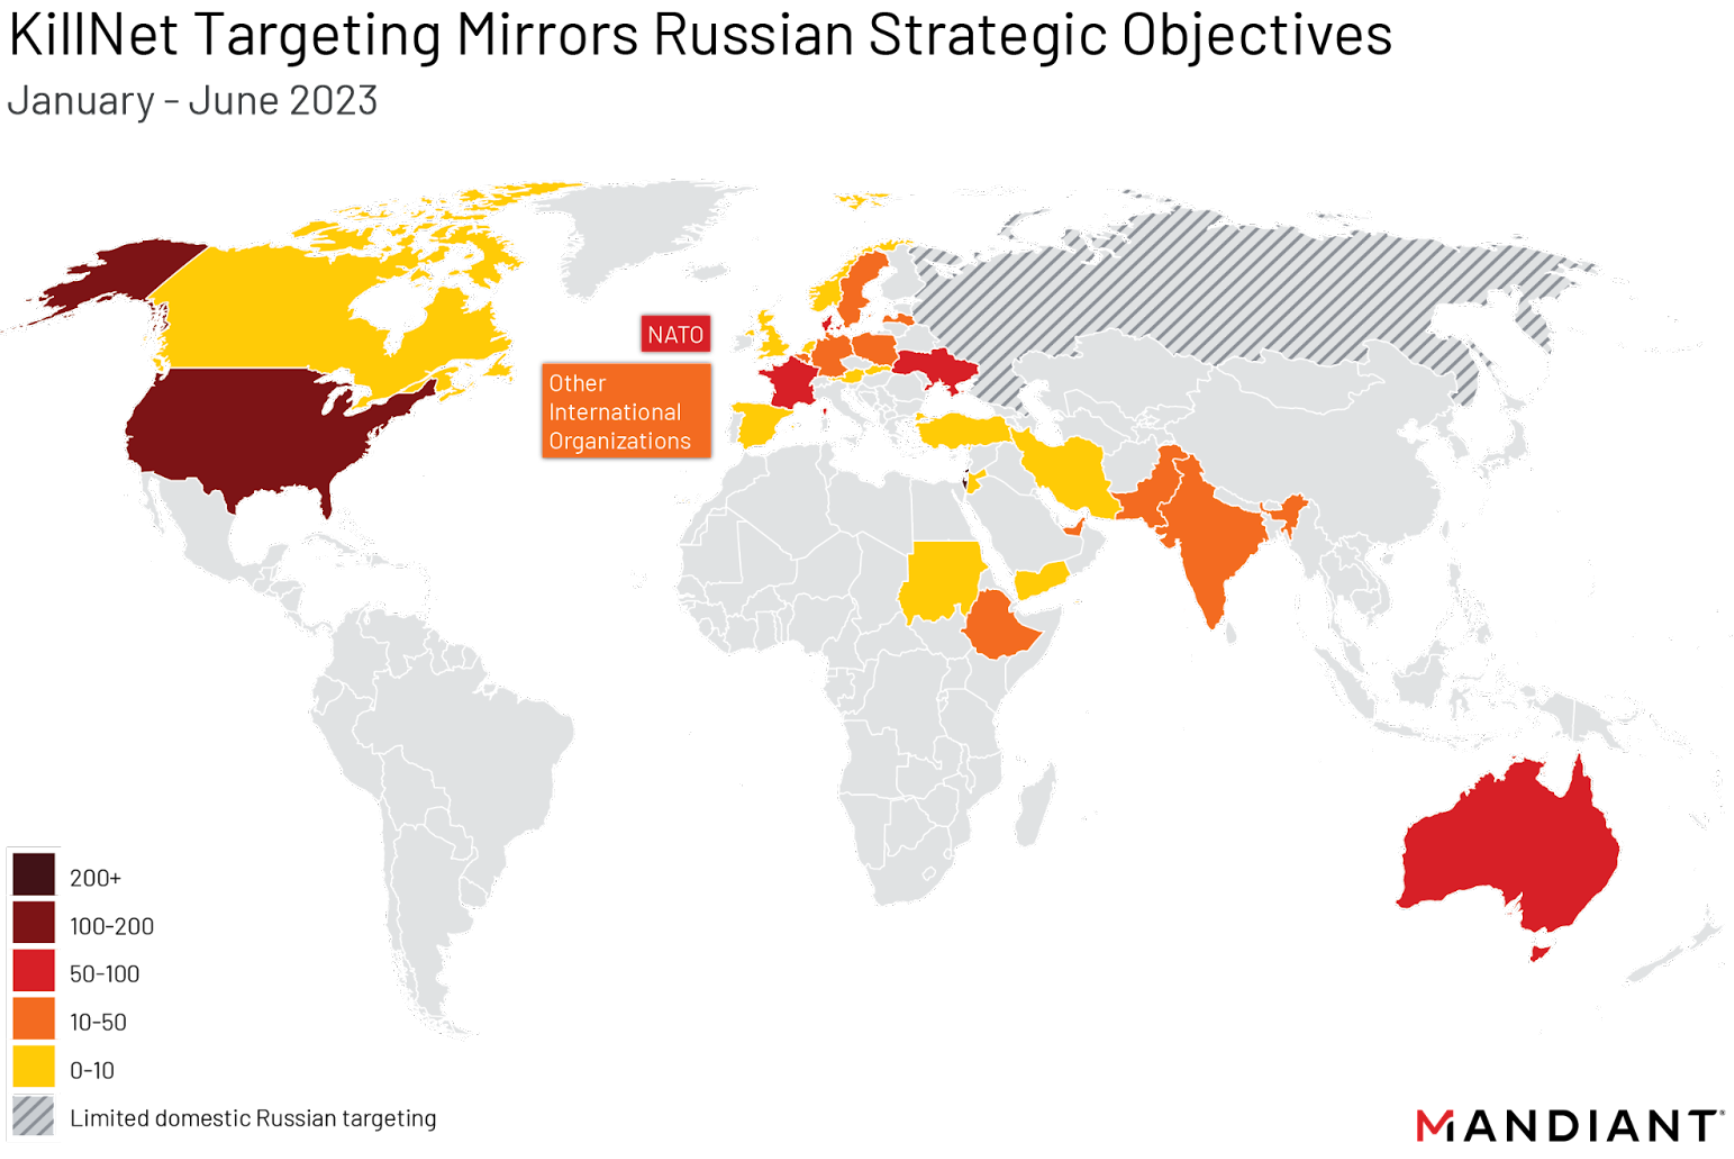
\includegraphics[width=0.8\textwidth]{Images/killnet.png}
\caption{\textit{Killnet attacks overview by \textcite{mandiant_2023_killnet}}}
\label{killnet.png}
\end{figure}

From the Ukrainian side, Anonymous and Anonymous Italia have been the primary actors in the field, excluding the government-affiliated IT Army of Ukraine. One of their objectives was to disrupt government websites and telecommunications. Remarkable action was the hack of several Russian televisions to show Russian citizens an independent coverage of the war in Ukraine\footnote{For more information: https://www.rferl.org/a/russian-tv-hacked-ukraine-anonymous/31740663.html}, since almost all the media are not allowed to diverge from the government perspective. 

Since February 2022, the threat actors number has increased constantly. As minefields or unexploded that would be difficult to find and disarm before some other incident after war, also the hacktivists will not cease to be active and other \textit{missions} will be found. 

\begin{figure}[H]
\centering
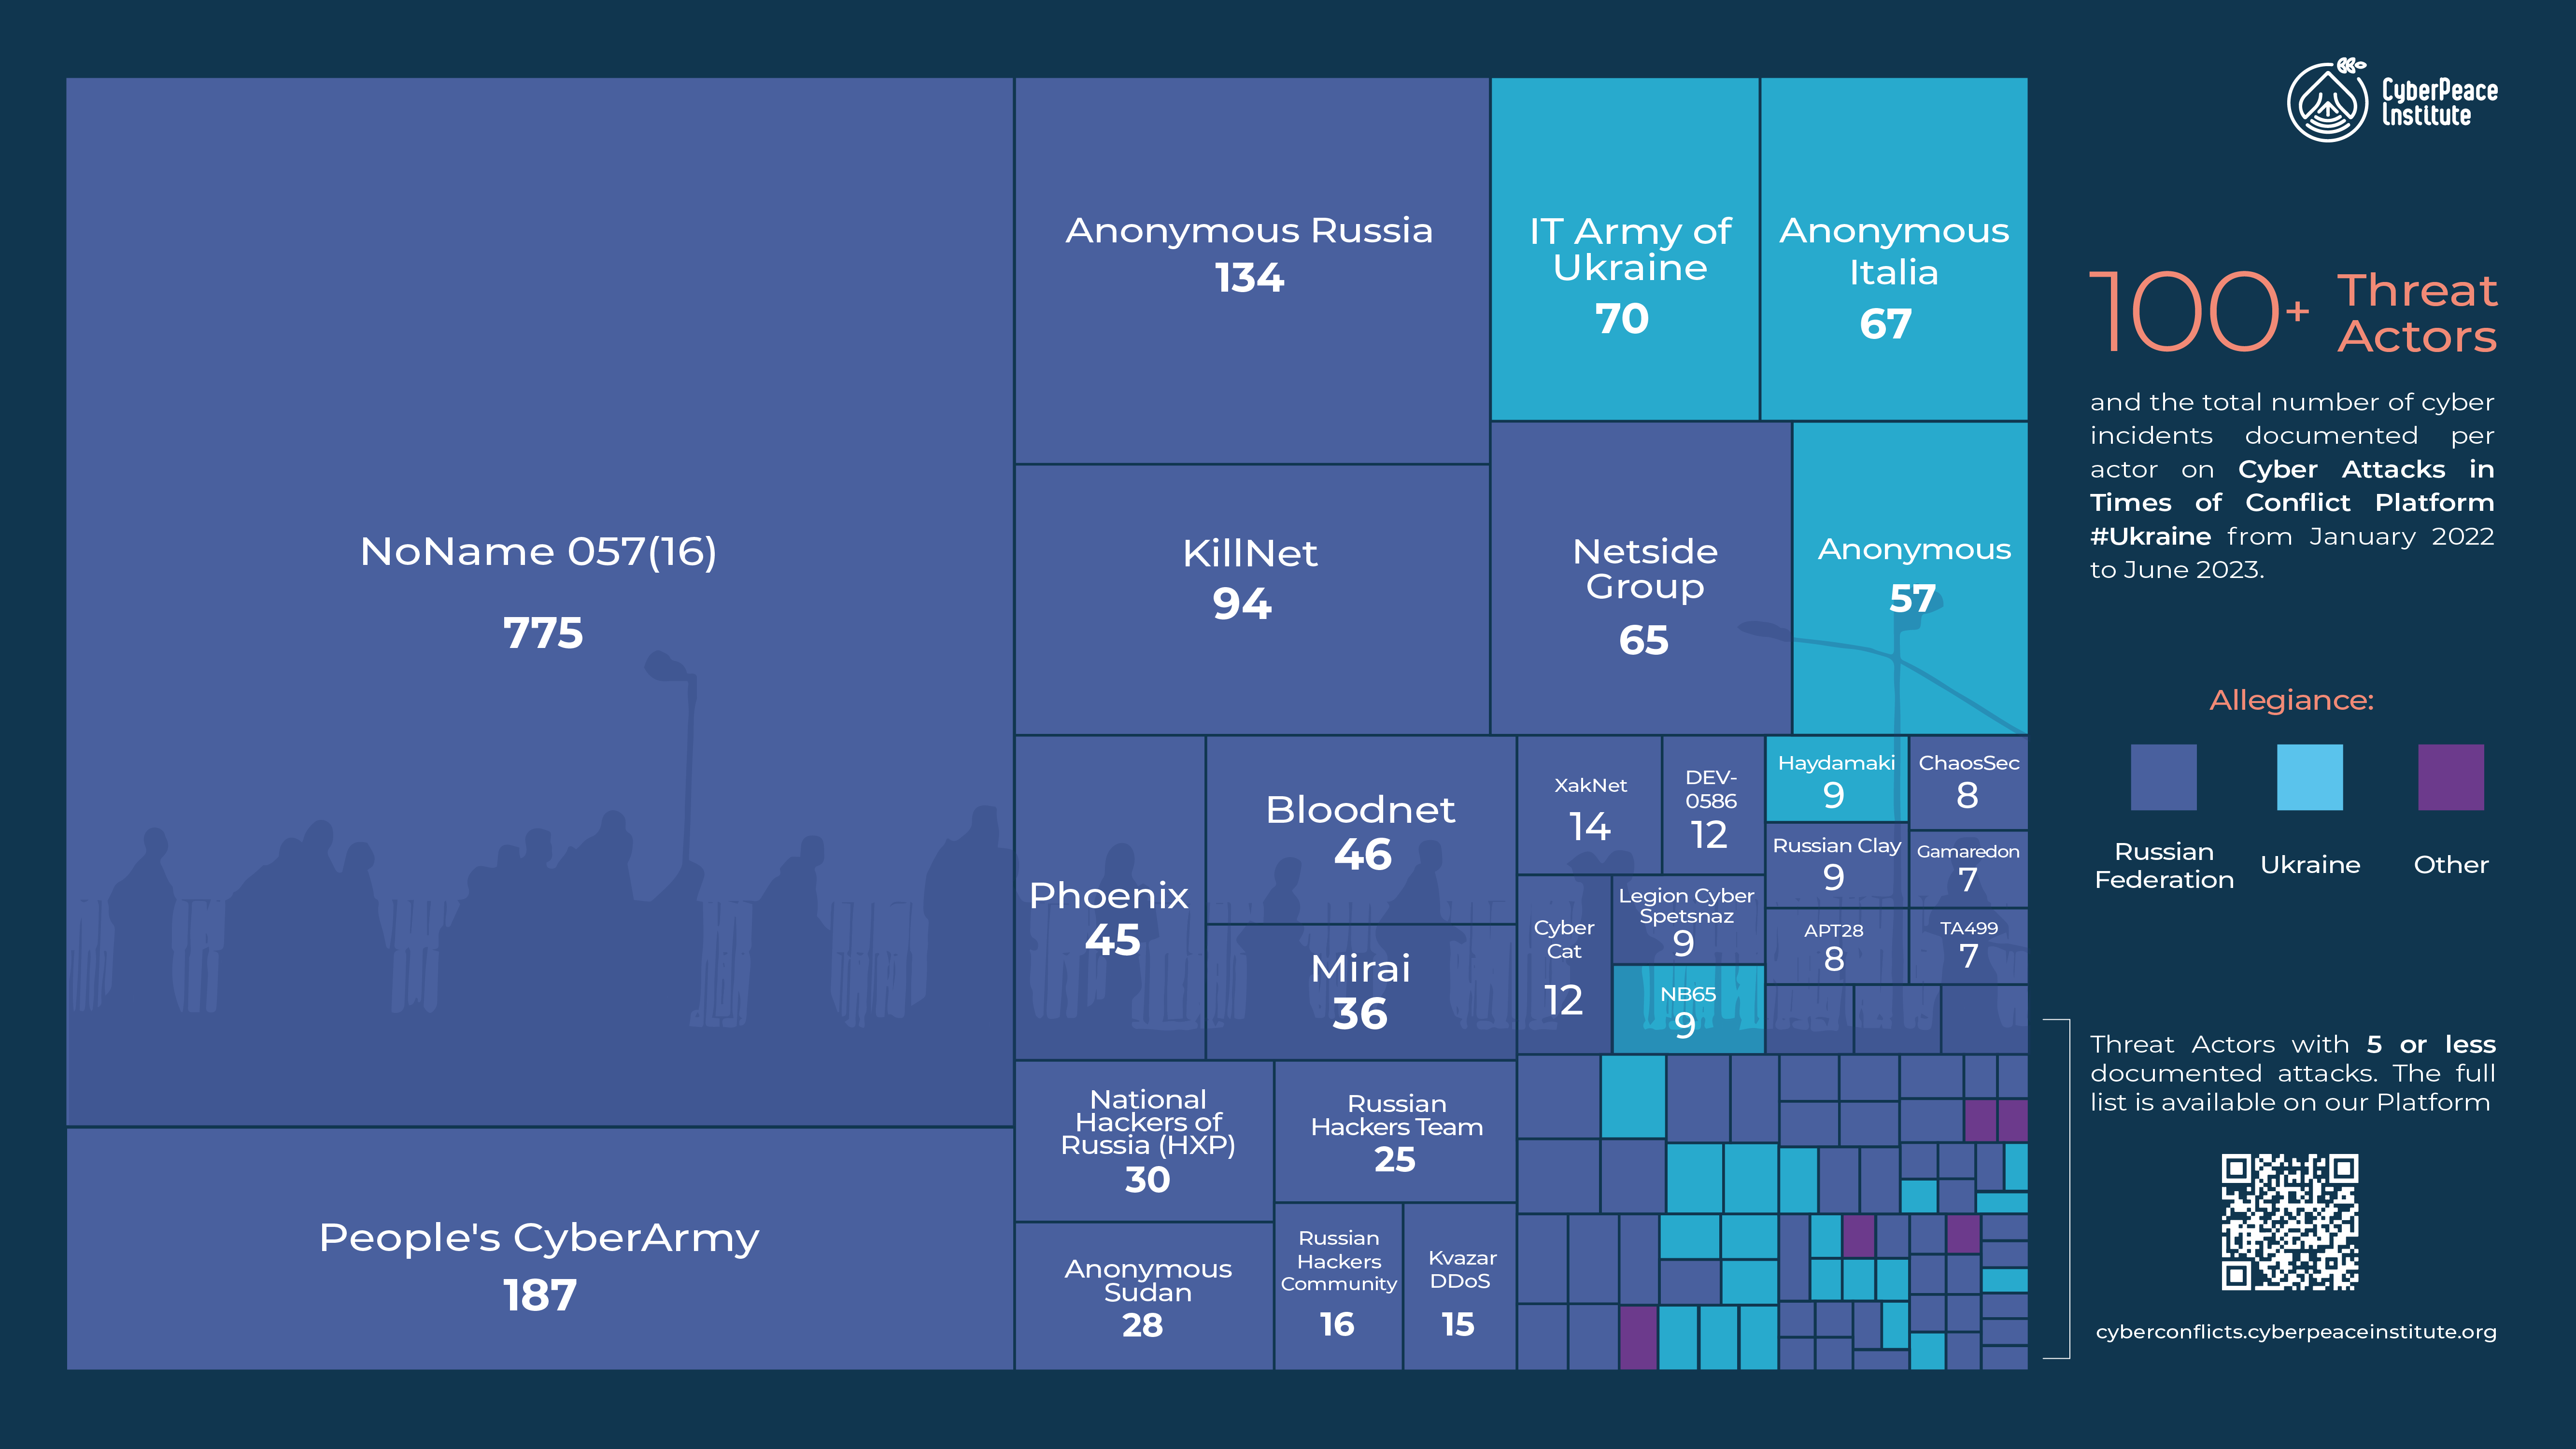
\includegraphics[width=1\textwidth]{Images/actors.png}
\caption{\textit{Threat actors overview after Russian Invasion of Ukraine by \textcite{cyberpeaceinstitute_2023_cyber}}}
\label{actors.png}
\end{figure}


\section{Conclusion: Russian Cyber Failure and Lessons to Learn}

Russian cyber operations could have experienced the same outcome as their kinetic counterpart without meeting the expectations of what was considered one of the best militaries in the world. Both cyber and military groups were unprepared to sustain long-term conflict. As Wilde stated:

\textit{Russian war-planning has long been underpinned by the assumption that it would be “the militarily inferior party in a regional or large-scale war against a technologically superior adversary.”  This tendency, alongside overly secretive and ill-informed pre-invasion planning, appears to have been in effect as Moscow (and the West) overestimated its own abilities and underestimated Ukraine’s, precisely during the period that its own doctrines deemed as most pivotal for information warfare \autocite{wilde_2022_cyber}}

The Russian VIO could not be compared to the United States Cyber Command, which has demonstrated its capabilities during cyber operations against ISIS. In contrast to their American counterparts, Russians are missing central Command \ and control, which could fill the structural problem that Russian cyber troops are affected by. Furthermore, the fragmentation of cyber fires does not help Russians. Some several cyber vigilantes and hacktivists sometimes conflict with each other \autocite{cyberpeaceinstitute_2023_cyber}. Russia lost the information war, both internally and internationally, while cyber operations were far from strategic assets. Hence, several scholars have stated that this war has shown that cyberspace is not yet a strategic domain. However, this war demonstrated that Russia’s cyber capabilities are not best suited for a military scenario differently from peacetime, while simultaneously confirming at the same time the problematic coercive issue of cyber operations. Studying the application of cyber operations during contemporary war scenarios is invaluable for acquiring knowledge, and the ongoing conflict between Russia and Ukraine is a crucial milestone in the development of the cyber field.

 
This case study allowed us to gain important insights and lessons learned regarding cyber capabilities during war. To link the key characteristics of cyber capabilities and capacities to the power’s projection, we will use the framework developed by \textcite{vanhaaster_2016_assessing}. The framework helps us to distinguish the political, informational, economic and military dimensions of them. 

\begin{table}[h]
    \centering
    \caption{State’s Power Instruments and Cyber Capacities}
    \label{tab:power-instruments}
    \begin{tabular}{|c|p{8cm}|}
        \hline
        Power Instrument & Capabilities \\
        \hline
        \textbf{Political} & 
        \begin{itemize}
            \item Deterrence
            \item Political Alliances
            \item Involvement of Private Sector
            \item Awareness campaign aimed at SMEs and Public Administrations
        \end{itemize} \\
        \hline
        \textbf{Informational} &  
        \begin{itemize}
        \item Intelligence gathering
        \end{itemize} \\
        \hline
        \textbf{Economical} & 
        \begin{itemize}
            \item Protect Critical Infrastructure
            \item Invest in Skills and Infrastructure
        \end{itemize} \\
        \hline
        \textbf{Military} & 
        \begin{itemize}
            \item Integration of Cyber-Kinetic (C\&C)
            \item Use of Preventive (Offensive) Attacks
        \end{itemize} \\
        \hline
    \end{tabular}
\end{table}



\textbf{Political}

The deterrence has changed its form since the nuclear confrontation during the Cold War. Making the attack more costly than the defence is one of the key features of deterrence in cyberspace, understood as deterrence by denial \autocite{nye_2017_deterrence}. As we analysed in the chapter, cyber operations to physically destroy critical infrastructure were less relevant instead of operations to disrupt or gather intelligence. Firstly, the destructive cyber-attacks are more expensive than the defence framework to counterattack it. For instance, the Stuxnet operation cost \$300 million against \$14 million for the defence \autocite{slayton_2017_what}. The Stuxnet operation, however, was only the first successful offensive operation of this type, which required years of preparation. This type of operation during wartime is less important from the operational perspective due to the planning and the scope. Why a country at war should use a million-dollar cyberattack to disrupt a critical infrastructure when it could use kinetic weapons? The Viasat hack was indeed necessary to disrupt the satellite military communication and to surprise the military counterpart with a full-scale offensive. However, for how much it was well executed, Ukraine (and its allies) has rapidly minimized the issues with other satellite providers (such as Starlink). 

This cyber realm of this war also represents something old in the history of conflict. Alliances can change the course of the war. The support of the Western countries was and is at the time of writing one of the main reasons for the resistance of Ukraine. The value of the cooperation since the Crimea annexation in 2014 has continuously increased. Ukraine's cyber policy has been revolutionised and conforms to NATO standards, abandoning the Soviet style of information war. Moreover, the alliance does not only benefit one part, but the Ukrainian experience was a big value for shaping NATO tactics even in cyberspace. 

Incorporating the private sector into national cyber policies, even during wartime, serves as another significant factor contributing to Ukraine's resilience. The role of big tech companies and their experience in the cyber field have been recognized by scholars. Notably, the disparity between national cyber capabilities and those possessed by the private sector in areas such as cyber threat intelligence and cloud services is evident. This experience presents a dilemma regarding the outsourcing of certain cyber defensive tasks to the private sector.

The increasing collaboration between the private sector in cyberspace and the government presents a unique dynamic, It has been acknowledged that these alliances frequently have cyber capabilities that are equal to or even better than those of state actors. This underscores the ongoing process of de-sovereignisation of defence, attributed in part to the forces of globalization. As a result, this evolution tests conventional national defence borders and highlights the importance of public-private partnerships in enhancing a country's cyber resilience.

A thorough awareness campaign aimed at SMEs and Public Administration should be a political priority to improve their capacity to fend off interruptions, even relatively manageable DDoS attacks. Due to their distinctive nature, hacktivists' actions have attracted a lot of attention during this battle. These cyber actors have maintained a high profile by publicly claiming responsibility for their attacks and openly identifying their victims. Notably, there have been instances where the websites of SMEs and public entities fell victim to prolonged, consecutive cyberattacks. The awareness campaign is designed to prompt proactive thinking within the management of these organizations. It serves as a response to warnings of potential targeting and aims to equip them with the knowledge and resources necessary to prevent or mitigate cyber threats effectively.

\textbf{Informational}

Intelligence gathering during wartime is the cornerstone not only for cyber operations but also for kinetic ones. During pre-war, intelligence served to shape the operational and tactical level avoiding that troops navigate in the shadows. The main reason for the Russian failure is often associated with an intelligence failure, since 3-day military operations were expected, with the Ukrainian army laying down their weapons. Russia has few times attacked Ukraine with kinetic weapons on the logistic sites where Western types of equipment were delivered, underlying the difficulties in gathering information. On the other side, Ukrainians with open source intelligence techniques have discovered the location of Russians who were using social media to post videos and photos on the frontline and while using dating app \footnote{A recent case study was analysed here: https://www.huckmag.com/article/how-tinder-became-a-weapon-in-the-russia-ukraine-war}.

\textbf{Economical}

Since 2014, Ukraine has been repeatedly targeted with cyberattacks on its critical infrastructure, including power grids, transportation networks, and financial systems. While some of these attacks were unsuccessful, the \textit{NotPetya} attack, in particular, caused significant disruptions to Ukraine's energy infrastructure. The ramifications of such cyber incidents serve as a stark reminder of the need for substantial investment in safeguarding critical infrastructure. This imperative isn't a mere rhetorical expression; it's a pragmatic policy aimed at nurturing a skilled workforce to enhance cyber resilience. Whether one is involved in offensive or defensive cyber operations, the core skill sets required remain the same. The creation of highly specialized units dedicated to countering cyber threats is a key determinant of success in this domain, as well as training and educational programs with these specific aims. In a human-crafted environment, it is the human factor that can make all the difference.

\textbf{Military}

This conflict has shown that we are far from strategic use of cyber operations due to their lack of integration with kinetic weapons and strategies. A unified Command \& Control for both kinetic and cyber operations was not present for both countries involved, as well a few offensive capabilities were deployed. In the Ukraine-Russia War, cyberspace was less used in a militarized manner, for what was possible to see from open sources. The failure of the integration of both instruments lies down to the organisational issues, lack of training and workforce and military/political will.  Cyber operations have been difficult to incorporate into the normal defence planning process, which is usually focused on a single theatre and allotting troops and weapons by phases of conflict. Cyber operations struggle with assured access, good estimates of effectiveness or extent of damage, or even certainty about how long they will work \autocite{lonergan_2021_cyber}. As \textcite{baetman_2022_russias} stated, the effectiveness of integrated cyber-kinetic fires depends on the level of coordination between cyber and kinetic operations. In some cases, cyber and kinetic fires may achieve unity of purpose through loose alignment or close coordination, while in other cases, their effects may be less cumulative or even unintended. The accumulated experience with cyber weapons has not yet achieved the same maturity as that with kinetic weapons \autocite{dykstra_2020_differentiating}. 




\chapter{Towards an EU cyber strategy?}

After exploring the concepts essential to develop a coherent approach for our analysis, this section will dive into the role of the European Union (EU) as a cyber actor. The analysis highlights how academic literature observes the EU’s role and identifies critical issues that emerge in its cyber posture. As mentioned in the previous section, securitization is a fundamental aspect of cybersecurity. Since 1957, the EU has played a significant political and economic role in the international arena. Despite the failure of the treaty to establish the European Defence Community and the increasing dominance of NATO, the EU lost its initiative to become more militarily active until the outbreak of the war in Ukraine. Furthermore, the EU has been a guiding force in the cyber domain, from a regulatory perspective. At the same time, the EU faces challenges in several areas. One such area is the fragmented nature of cybersecurity within the EU, which could have an impact on the coherence of EU policy, since there are different national cyber strategies. The renewed emphasis on cyber defence by the EU in recent times has also highlighted the need to build cyber capabilities in the EU. Despite these challenges, the European Union has a defined diplomatic approach to cyber concerns and offers Member States a tool for retaliation. Lastly, this chapter addresses the issue of institutional overlap between the EU and its Member States. Cyber power differs from other types of power. Although information has been considered one of the ancient types of power (Sun Tzu and Thucydides as examples), cyberspace has created a new domain of confrontation in which no geographic borders are present. Thus, the recognition and manifestation of cyber power do not follow the classical theoretical framework.

The EU's concerns about cyber issues became more relevant after the Estonia cyberattack in 2007, leading to the creation of regulations and directives, such as Network and Information Security (NIS) regulation, and the establishment of bodies like the European CyberCrime Centre.


According to Dunn Cavelty (2018), the EU's cyber policy can be divided into three main areas.

\begin{enumerate}
    \item Network and Information Security
    \item Fight against cybercrime
    \item(Military) Cyber Defence and foreign policy 
\end{enumerate}

In this context, the focus will be on the third aspect, which is related to cyber defence and the foreign policy aspects of the EU's cyber power.

The European Union has been considered a success story in the post-1945 era, primarily because of its economic advances and the creation of a single monetary system. However, the Union appears to be less advanced in terms of foreign policy and security. Scholars, such as \textcite{sliwinski_2014_moving}, have been sceptical about the role of the EU, especially in the cybersecurity field. The main critique lies in the intergovernmental nature of the decision-making process behind (cyber) security aspects. According to \textcite{sliwinski_2014_moving}, organisations such as NATO are more suitable as cyber actors because of their real capabilities, adaptiveness, and role in facilitating cooperation, unlike the intergovernmental coordination pursued by the EU. Other authors, such as, \textcite{klimburg_2011_cybersecurity} suggest a division of labour between NATO and the EU in cyberspace. The EU should focus primarily on critical infrastructure protection and develop regulations aiming to harmonise Member States' legislation, mainly regarding the civil aspect. On the other hand, NATO should be more involved in the military aspect of cyberspace, benefiting from the Command and Control (C\&C) advantages within the Atlantic Alliance. This approach reflects the CFSP-NATO relationship.

Furthermore, in recent times, the EU has developed new strategies and capabilities to take concrete action in this direction. For instance, the EU has promoted more standardisation through the establishment of the European Cybersecurity Certification Framework (ECCF) with the EU Cybersecurity Act. This framework affects both the military and civil spheres and aims to enhance cyber capabilities within the EU.

In addition, the cooperation between NATO and the EU has increased on cybersecurity issues. For example, the NATO\textit{ Computer Incident Response Capability} (NCIRC) and the \textit{Computer Emergency Response Team – European Union} (CERT-EU) have been operating daily since 2016 \autocite{eeas_2016_eu}, with the aim of improving cyber incident prevention, detection, and response. NATO-EU cooperation is significantly more advantageous than acting alone, primarily because cyberattacks during peacetime primarily target civil society and critical infrastructure. Additionally, hybrid wars and disinformation campaigns have been conducted within a grey zone, where traditional methods to counteract them are insufficient.

However, during the Russian invasion of Ukraine in 2022, the relationship between NATO and the EU on security issues has developed further, requiring a new investigation to understand the patterns and how it affects the cybersecurity approach of the two organisations in wartime. This work will include this analysis with the aim of filling the gap in cybersecurity cooperation/coordination between the EU and NATO during wartime.

\section{EU Cyber Strategy: an historical perspective on researching resilience and coherence}

The European Union is gradually emerging as a significant player in the cybersecurity domain and aspires to achieve coherence \autocite{carrapico_2017_the}. Assessing the efficiency of EU policies is a challenging endeavour, particularly when applied to novel domains, such as cyberspace. From a theoretical standpoint, enhanced coherence could amplify the effectiveness of EU policies, especially in shared competencies such as cyberspace among Member States. According to \textcite[1256]{carrapico_2017_the}, \textit{coherence can be evaluated through institutional coordination and a shared understanding of security}. Specifically, institutional cooperation is crucial for assessing the development and contribution of institutions to the policy cycle as well as identifying potential overlapping issues, both in terms of political and operational tasks. On the other hand, the shared concept of security enables Member States to develop a comprehensive strategic framework, such as the EU Strategic Compass, facilitating further discussions and integration of security matters.

Since the 1990s, the EU's approach to cybersecurity has undergone a significant evolution, shifting from its initial focus solely on cybercrime to adopting a more comprehensive understanding of cybersecurity. The publication of cybersecurity strategies has played a vital role in promoting coherence within EU actions and preparing a region for future development in this domain. Initially, the EU indirectly addressed cybersecurity concerns by associating the information and technology sector with the Single Market. During the 1990s and the early 2000s, several non-legally binding instruments were approved to counter cybercrimes. Key milestones in this period were the conclusion of the \textit{eEurope 2002 Action Plan, promoting an Information Society for All, and the Commission Communication on Improving the Security of Information Infrastructures and Combating Computer-related Crime (2001)} \autocite{carrapico_2017_the}. However, a significant shift occurred in 2004, prompted by the emerging threat of terrorism, leading the EU to adopt legally binding measures. Simultaneously, in the same year, the \textit{European Network and Information Security Agency} (ENISA) was established to facilitate the exchange of best cybersecurity practices. One notable development was the \textit{Council Framework Decision on Attacks against Information Systems}, which marked a crucial milestone in adopting a transnational approach to cybersecurity within the European Union. This framework is centred on three key pillars: addressing cybercrime, protecting critical information infrastructure (CIIP), and bolstering cyber defence \autocite{carrapico_2017_the}. 

The first document which clearly proposed a strategic approach to the domain was the \textit{EU’s Cybersecurity Strategy} published in 2013. It embedded the three pillars and highlighted the role of the EU in securing economic infrastructure and increasing resilience. According to \textcite{kasper_2021_the}, the new\textit{ EU Cybersecurity Strategy for the Digital Decade}, approved in 2020, highlighted the coherence issue within cybersecurity and other influenced policy areas, conducting steps forward on cyber defence with a more political lens. In this regard, both scholars agree on the EU's ambition to establish itself as a global cyber power, notwithstanding its regional organizational nature. The \textit{NIS Directive (2016/1148)}, the first horizontal legislation on cybersecurity \autocite{markopoulou_2019_the}, constituted a real act on cybersecurity that complies with the EU’s strategy. The directive aims to protect critical infrastructure and IT services from deliberate incidents that can cause disruption. It addresses compliance obligations for addressees and member states' obligations to their respective national strategies and cooperation at the EU level. In this regard, ENISA played a key role in facilitating cooperation between Member States and following the adoption of the NIS Directive in national legislation. The Directive has been updated (2022/2555), affecting a larger group of entities, energy providers or airports, and medium-large enterprises, categorising them between essential and important entities \autocite{enisa_2023_nis}. 

Moreover, \textit{Regulation 2019/881}, also known as the \textit{Cybersecurity Act}, introduced several measures to enhance the EU's cybersecurity capabilities and strengthen its resilience against cyber threats. The Act introduced a comprehensive approach, empowering the European Union Agency for Cybersecurity (ENISA) to coordinate the framework. It allows for voluntary and mandatory cybersecurity certification of ICT products and services, with a focus on critical technologies, through a high-level certification scheme. Additionally, the Act establishes the European Cybersecurity Certification Framework Cooperation Group to ensure the harmonised development and application of certification schemes. Furthermore, it places a strong emphasis on raising cybersecurity awareness and promoting the adoption of certified products and services to enhance the overall cybersecurity posture \autocite{europeanparliament_2019_regulation}. 

\begin{figure}[H]
\centering
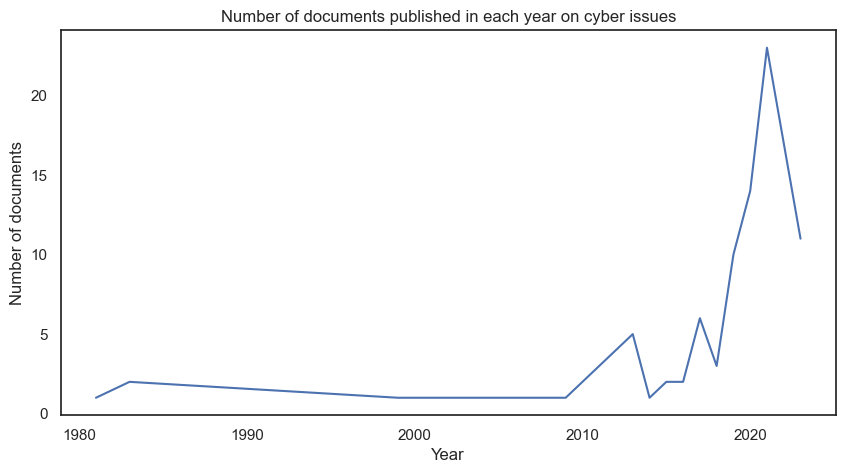
\includegraphics[width=1\textwidth]{Images/eurlex.png}
\caption{\textit{EU Legislation and International Agreements Related to Cyber Issues: 1981 to 2023. The data was retrieved from EUR-Lex. For more information about the keywords used for scraping. For a detailed explanation of the data retrieval process, see Appendix \ref{def:eurlex}}}
\label{fig:eurlex.png}
\end{figure}

Over the years, there has been a noticeable increase in the EU's actions concerning cybersecurity. This can be observed through a search on EUR-Lex for legislative and international agreements that encompass cyber-related terms. Notably, there has been a significant surge in publications post-2010, indicating that the EU has elevated cybersecurity to a position of high priority in its policymaking process. All the legislations proposed, embed a multistakeholder approach also reflected in the \textit{EU’s principle of shared responsibility for the effective security of cyberspace} \autocite[6]{christou_2014_the}. The EU has continued to regulate the cyber domain by forging connections with other policy areas, such as the economy, human rights, and security. This integrated approach is crucial for enhancing policy efficiency; however, it requires more institutions to be involved.


\section{Cooperation between institution}

The\textit{Cybersecurity Institutional Map}, created by ENISA, highlights the fragmented and decentralised nature of EU governance on cyber issues. ENISA identifies 18 distinct functions, including R\&D, capacity building, attribution, response to hybrid threats, and the development of cyber resilience. These functions are categorized into four communities: Justice in Cyberspace and Cybercrime Community, Cyber Resilience Community, Cyber Defence Community, and Cyber Diplomacy and Policies Community. Numerous institutions are involved in these diverse responsibilities. The European Agency for Cybersecurity, DG for Communications, CERTs, and EDA are just a few examples that constitute the cybersecurity governance architecture of the EU. Upon initial examination, this hypothesis suggests a potential overlap of functions between several institutions and agencies. As is evident from the Figure \ref{institutional_map.png}, numerous institutions are engaged in similar functions, albeit with varying degrees and scopes. The initial cluster analysis identifies three primary groups: one primarily judicial, another focused on military affairs, and a third encompassing a broader range of functions, which includes the Commission’s DGs and European Agencies, such as The European Defence Agency and ENISA, following the same division between internal and external security issues that have been traditionally applied to European governance \autocite{miadzvetskaya_2021_the}.

\begin{figure}[H]
\centering
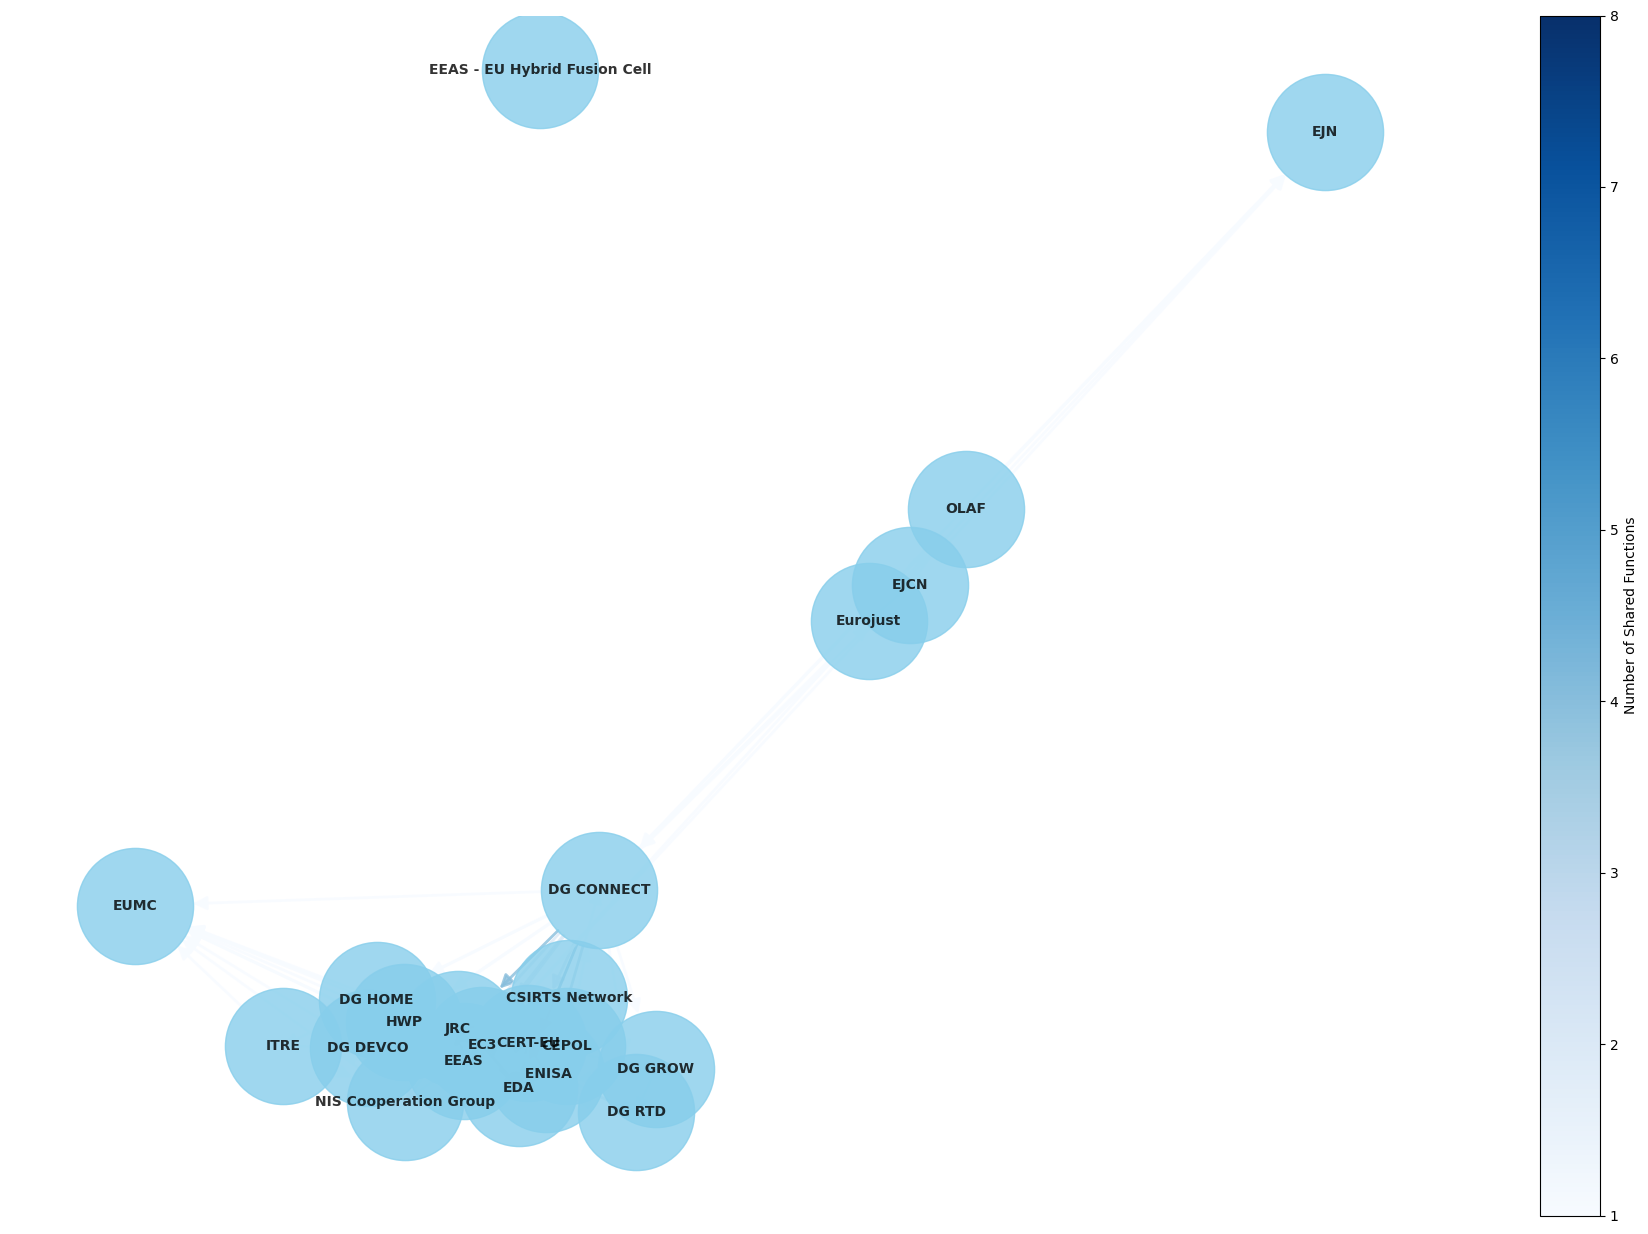
\includegraphics[width=1\textwidth]{Images/institutional_map.png}
\caption{\textit{Clustering ENISA's Cybersecurity Institutional Map showcases EU's diverse institutions collaborating on shared functions in the cyber domain.}}
\label{institutional_map.png}
\end{figure}

\section{Cooperation between Member States}

It is crucial to consider the level of cooperation among Member States in this field, as \textit{despite the increasing Europeanization, cybersecurity in Europe remains solely a national responsibility} \autocite[13]{renard_2014_european}. Several projects at the EU level, such as the \textit{Permanent Structured Cooperation} (PESCO) and initiatives by the European Defence Agency, foster cooperation among participating countries. However, participation in these endeavours remains voluntary, with only a few countries involved. \textcite{kasper_2021_the} emphasizes that \textit{there are no cyber islands} within the EU, highlighting the need for a comprehensive strategy, primarily among EU member states and subsequently with third parties.  The existing literature lacks robust analysis of the EU's role in promoting active cooperation in cybersecurity, largely due to the reasons discussed earlier, as scholars perceive the EU as less capable of enhancing cooperation in the security field compared to other organizations like NATO and OSCE. The concept of EU coherence has some key features to fully understand it. Firstly, there is the prevailing notion that the EU acting as a unitary actor would result in a more \textit{effective} EU. However, this assumption is not inherently evident, particularly in the realm of foreign policy, where the EU has often prioritized unanimity over effectiveness \autocite[5]{missiroli_2001_occasional}. Additionally, it is worth noting that a policy can be effective without necessarily being consistent, as exemplified by metaphors like \textit{carrot-and-stick} or the concept of \textit{good cop-bad cop} \autocite[5]{missiroli_2001_occasional}. Nonetheless, the EU has laid the groundwork and provided a general framework for new instruments that have been increasingly utilized in recent years, such as cyber diplomacy and cyber defence.

\section{Digital Sovereignty}
After the COVID-19 pandemic, the European discourse on resilience and sovereignty has gained greater relevance compared to the past, particularly encompassing various policy areas, including technology and digital domains. The concept of technological sovereignty was first introduced in the 2020 Cybersecurity Strategy and the Strategic Compass, both aimed at promoting the Union's strategic autonomy. However, this idea of sovereignty stands in contrast to the principles of multistakeholder internet governance, which the EU itself supports, emphasizing openness, inclusion, bottom-up collaboration, and consensual decision-making \autocite{pohle_2020_digital}. The EU's perspective on sovereignty revolves around a more political and strategic realm rather than a purely operational one. It perceives cyberspace as a battlefield, where the EU must ensure the security of its citizens against actors, including non-state ones, that challenge the principles of openness and security in the digital arenas. \autocite{andrbarrinha_2022_speaking}. Consequently, the EU has intensified efforts to achieve strategic autonomy in cyberspace through internal and external policies. From an internal standpoint, the EU has introduced risk management-based regulations, exemplified by the NIS Directive and the GDPR \autocite{andrbarrinha_2022_speaking}. On the other hand, the EU has also focused on other policy areas relevant to cyberspace security, investing in strategic sectors.

The European Union and its development since the Treaty of Rome have followed a liberal pathway. It has guaranteed (with different degrees of evolution) the freedom of movement of goods, services, persons and capital. However, globalisation showed new rivals both in economic and political terms. Countries such as China and India have exploited the flourishing European Single Market (ESM) for different purposes: to gain from trade by delocalising their domestic firms and, most important, by investing in those firms that could guarantee the necessary technological know-how. Therefore, the EU guarantees the basis of competition in the ESM (Articles from 101 to 109, TFEU), freedom of establishment in the Union (Articles from 56 to 62, TFEU), and freedom of capital (Article 63, TFEU). Although some barriers have been raised, despite the liberal philosophy accompanying the Union. In the last few years, emerging markets' FDI has affected European strategic sectors. It is dangerous for European stability and integrity when these investments are made by a political (and economic) rival such as China. Consequently, the EU has introduced the \textit{Regulation 2019/452}, designated as the FDI Screening Regulation, as an economic securitisation in a liberal economic context \autocite{shilder_2022_securitisation}. It does not define a new European mechanism for screening foreign investments, but aims to coordinate the Member States. The critical aspect of the Regulation refers only to the security and public aspects of the screening of FDI (Article 1 of Regulation 2019/452), similar to how the Member States may restrict the free movement of capital from third countries (Article 65, TFEU) and regarding hostile investments (Article 207, para.2, TFEU). The economic terms are completely excluded for not undermining the liberal principle of the Union. The Court of Justice of the European Union remarked that FDI falls within the exclusive competence of the EU, while indirect investments, such as portfolio investments, are shared competence \autocite{cjeu_2015_opinion}. In addition, in the Regulation are listed those sectors that could be strategic for the Member States, such as critical infrastructure, both virtual and physical, critical technologies and their dual use (artificial intelligence, semiconductors, among others), media, energy, and raw material material supply chain. The Regulation refers to the rights of the Member States to protect their vital interests (under Article 346, TFEU). In addition to other regulations, such as the Chip's Act or the AI Act, that proactively impact the securitisation of technological domains by establishing barriers against actors who fail to comply with the EU's values, the pursuit of strategic autonomy has emerged as a catalyst for redefining foreign policy instruments in policy areas that cannot be confined to a defined border between internal and external policies.

\section{Cyber diplomacy of the EU}

The EU cyber diplomacy is aimed at shaping the global cybersecurity landscape according to EU values and interests. As stated by the Council of the EU in its guidelines on external EU cyber capacity building, the EU should focus on cooperating with partner countries and regions as a strategic building block of the EU’s cyber diplomacy efforts to promote and protect human rights, gender digital equality, the rule of law, security, inclusive growth, and sustainable development \autocite{counciloftheeuropeanunion_2018_eu}. This approach explains how the EU cyber diplomacy strategy is more focused on cyber issues that impact societies and economies, rather than a purely security-orientated approach to the problem. However, this strategy has experienced a change in its strategic posture due to the Russian invasion of Ukraine. In fact, the EU highlights in its Strategic Compass the need to \textit{develop the Cyber Diplomatic Toolbox and establish a cyber defence policy in the EU to be better prepared for and respond to cyberattacks} \autocite{eeas_2022_a}. The European Union recognised the need for a concerted diplomatic response to tackle malicious cyber activities, leading to the introduction of the \textit{ Cyber Diplomacy Toolbox} (CDT) in June 2017 \autocite{detomascolatin_2020_si}. The primary objective of the CDT was to establish an effective framework for a united EU diplomatic response, aimed at mitigating and deterring potential aggressors in the cyber domain from undermining the political, security and economic interests of the Union \autocite{counciloftheeuropeanunion_2017_council}. To achieve this goal, the framework involved the imposition of targeted restrictive measures against both entities and individuals engaged in malicious cyber activities. The extent of these measures was adjusted in proportion to different considerations, which included factors such as the size, extent, duration, strength, and consequences of cyber operations.


On 30 July 2020, a significant milestone was achieved when the Council of the European Union unanimously enacted restrictive measures targeting six individuals and three entities affiliated with \textit{Al-Qaeda} and \textit{ISIL} \autocite{counciloftheeuropeanunion_2020_regulation}. These measures were specifically directed toward those who were identified as being accountable for or having direct involvement in a range of cyberattacks perpetrated against the EU Member States. It was the first time that the Cyber Diplomatic Toolbox was used as diplomatic retaliation against individuals and entities involved in cyberattacks. This episode opens the path for a new diplomatic posture in cyberspace, which could lead to a cyber-sanction regime \autocite{moret_2017_the}. The Cyber Diplomatic Toolbox includes a range of diplomatic measures that can be summarised as preventive, stable, cooperative, and restrictive measures \parencite{miadzvetskaya_2021_the, counciloftheeuropeanunion_2017_council}. Preventive measures are the EU initiative to promote \textit{ confidence building measures} (CBSs), including third countries, with the aim of increasing cooperation and dialogue between the parties. The Cooperative measures encompass a diplomatic attitude for a peaceful resolution of the cyber incident. The stability measures refer to the declaration of the EU institutions on the general cyber trends or disruptive ones. Lastly, restrictive measures are proportionate to the scope, scale, and duration of aggressive behaviour in cyberspace \autocite{counciloftheeuropeanunion_2017_council}. To apply the so-called cyber-sanctions, the EU has avoided the \textit{attribution} problem by condemning individuals who were related to a particular cyber operation rather than directly a country \parencite{miadzvetskaya_2021_the, bendiek_2018_the}. 

Even if the securitisation role assumed a prominent role in the EU cyber strategy, it is not disjoined from the EU core values. For this reason, the EU’s relation on (not only) the cyber issue with countries that do not reflect those values (such as China or Russia), is not focused on cooperation, but emphasises them as strategic competitors, while assuming retaliatory behaviour against them. For instance, EU decisions to ban TikTok and to introduce limits to Chinese investment in the crucial sector (such as AI or critical infrastructure, even cyber ones) are just some of many examples of the determinant behaviour of the EU to protect and promote its values. In this regard, the pursuit of the EU’s values, even in the cybersecurity international landscape, represents a clear form of coherence. 

A global cybersecurity posture is characterised by a tendency to externalise EU cybersecurity \autocite{miadzvetskaya_2021_the}. This means that the EU recognises the interconnected nature of cyber threats and understands that effective cybersecurity cannot be achieved in isolation. Instead, the EU actively engages in cooperation and collaboration with other countries and international organisations to collectively address cybersecurity challenges.

According to \textcite{kurowska_2019_the}, the EU’s cyber diplomacy could engage in strategic narrative contestation to shape the cyber governance process more effectively. In addition, the EU has committed itself to the international principle of due diligence in cyberspace and improved the exchange of information with third parties to counter cyberattacks \autocite{bendiek_2018_the}. The due diligence has been promoted by controlling the export of dual-use goods \autocite{bendiek_2018_the}, as happened with the sanctions against Russia after the invasion of Ukraine. \textit{The defence area has been marked by a differentiated approach across the EU, and the cyber domain is no exception}  \autocite[426]{miadzvetskaya_2021_the}. The EU’s unanimity requirement makes it difficult to approve acts that deliberately consider a state as a sponsor for a cyberattack, as reflected in the different foreign policy strategies of the Member States. On the other hand, the European Union has achieved progress even with regard to cyber defence, a different instrument if compared to cyber diplomacy, but with the same goal. 

\section{European Cyber Defence}

Cyber defence has become a top priority for the European Union in recent years due to the rising cyber threats faced by member states.  The EU has introduced several regulations, policy documents, and initiatives to enhance cyber defence capabilities and cooperation among member states. In this scenario, the European Union have enhanced its power as a regulatory actor instead of a pure military one. With the EU Cyber Defence Policy Framework acknowledges cyberspace as the fifth domain of operations, alongside the domains of land, sea, air, and space \autocite{counciloftheeuropeanunion_2018_council}. Building normative blocks through Commission driven policy it has been a benefit for the Union considering that not every EU member has considered the cybersecurity as a top policy priority. 

With the creation of \textit{Joint Cyber Unit} (JCU), a new platform was proposed where EU institution, bodies and members could find a better place to improve operational cooperation, coordination, and information sharing. The JCU is also expected to play a role in the EU's response to cyber threats. The EU's Cybersecurity Strategy for the Digital Decade outlines the main objectives and priorities of resilience, technological sovereignty and leadership, and building operational capacity to prevent, deter, and respond. 

On the military perspective, the \textit{European Union External Action} (EEAS) and the\textit{ European Union Military Staff} (EUMS), have agreed on a military vision and strategy on cyberspace as domain of operation. 
In this document, the integration of cyberspace into crosscutting military domain are considered one of the factor which will impact of the freedom of action during military operation \autocite{eeas_2021_mil}, highlighting the importance of coordination of Command \& Control in the tactical and operational level. Both Diplomatic and Military offices emphasized the use of cyber operations as hybrid warfare and those challenges derived from it, making it difficult to apply standard crisis management plans. 

The vision recognizes that the EU has the capability to accomplish its objectives in the cyberspace domain as it does effectively in other domains of the CSDP missions; it has integrated the operations and missions establishing consistent cyber resilience and deterrence as well as established an integrated EU civili-military synergies in \textit{EU Common Security and Defence Policy} (CSDP).  The key takeaways of this strategic document are the capacities and capabilities needed to affirm EU Cyber Strategy under the CSDP. This comprehensive strategy encompasses various dimensions, including cultural adoption, operational capabilities, crisis planning, and international cooperation, with the overarching goal of establishing a stable and secure cyberspace for EU CSDP military operations and missions.

At its core, the strategy acknowledges that adversaries frequently operate below the threshold of armed aggression. This recognition propels the need for continuous adaptation to the evolving cyber threat landscape, marking a strategic shift towards resiliency, defensive actions, and deterrence. Understanding adversarial cyberspace operations as strategic campaigns becomes paramount, emphasizing a holistic cultural adoption that permeates through all levels of EU CSDP military operations. To operationalize this cultural shift, the strategy introduces a coordination and transition instrument as a key facilitator for implementing Cyberspace Operations capabilities. It calls for active involvement from EU institutions, Framework Nations, Member States, and partners. The rapid reflection of capabilities identified through the EU Capability Development Process (CDP) is essential, ensuring that the EU military remains agile in integrating new technologies and methodologies. Along with EU Member States, NATO remains a critical partner on developing a coherent cyber strategy. The partnership goes beyond the cooperation between Computer Incident Response Teams, including cooperation in technology acceleration programs such as \textit{DIANA}. 

From a regulatory perspective, the strategy implies adopting a regulation similar to NIS in the military field. This would result in comprehensive crisis management and interoperability across EU member states, facilitated by collaboration with ENISA.

The document also focusses on the informational gathering. It emphasizes the need for a permanent and federated cyber information sharing and fusion framework, complemented by appropriate processes and technical capabilities, highlighting once again the problem with the information sharing, even through partner actors.

Furthermore, the personnel and skills investment are considered the operational core of the strategy. The development of the Cyberspace\textit{ Education, Training and Exercise} (ETE) at all levels constitutes the core capability of EU cyber defence. As the war in Ukraine demonstrated, the operational skills are the pivotal aspect that involves both defence and offence during cyber operations. Even though the scope could be different (destructive, intelligence gathering, cyber defence or others), the skills to achieve the objective are not so different \autocite{slayton_2017_what}.  

Moreover, collaboration with industry, academia, and the cybersecurity market is emphasized for strategic insight and innovation. The strategy encourages the examination and utilization of opportunities with organizations like the  \textit{European Cyber Security Organisation} (ECSO), leveraging external expertise and fostering a collaborative environment.

Referring to the lessons to be learned and state’s power instruments/cyber capacities Table \ref{tab:power-instruments}, the \textit{European Union Military Vision and Strategy on Cyberspace as a Domain of Operations } has included all the issue presented on the Ukraine-Russia War case study. However, the implementation of those strategies and visions is less clear and further research on them is needed to assess if there have been practical step forwards or the document remained on the political discourse without being applied. 

On the other hand, the active engagement of the European Union (EU) in various  Permanent Structured Cooperation (PESCO) projects constitutes a tangible manifestation of the EU's commitment to translating political declarations into actionable strategies for cybersecurity \footnote{Behind the description, few information are availble on the PESCO projects due to their nature. You can find all the PESCO Projects here: https://www.pesco.europa.eu/ }. Among these initiatives, the\textit{ Cyber Ranges Federations} (CRF), coordinated by Estonia, exemplifies a collaborative effort to consolidate national Cyber Ranges, thereby enhancing cyber training, exercises, and research capabilities. The project underscores the EU's recognition of the need for a collective approach to address evolving cyber threats. In a parallel vein, the \textit{Cyber Threats and Incident Response Information Sharing Platform} (CTIRISP), spearheaded by Greece, reflects a strategic move towards more active cyber defence measures. By establishing a platform for sharing cyber threat intelligence among Member States, the initiative acknowledges the imperative of information exchange in fortifying national cyber defence capabilities. This shift towards proactive measures is indicative of a nuanced understanding of contemporary cyber challenges. The \textit{Strategic C2 System for CSDP Missions and Operations} (EUMILCOM), coordinated by Spain, signifies a targeted effort to enhance the command-and-control systems of EU missions globally. The project's modular and scalable approach underscores the EU's commitment to improving military decision-making processes and operational coordination, aligning with the evolving nature of cyber threats and their geopolitical implications Concurrently, the \textit{Electronic Warfare Capability and Interoperability Programme for Future Joint Intelligence, Surveillance and Reconnaissance} (JISR), led by the Czech Republic, underscores the EU's recognition of the importance of electronic warfare capabilities. The project's focus on a comprehensive feasibility study and potential joint concept adoption indicates a strategic approach to addressing gaps in existing electronic warfare capabilities. Lastly, the \textit{Cyber Rapid Response Teams and Mutual Assistance in Cyber Security} (CRRT), coordinated by Lithuania, manifests the EU's commitment to collective cyber resilience and response capabilities. The emphasis on deployable cyber toolkits and the provision of assistance to member states, EU institutions, and CSDP operations aligns with the recognition of the interconnected and collaborative nature of cybersecurity challenges.

\begin{figure}[H]
    \centering
    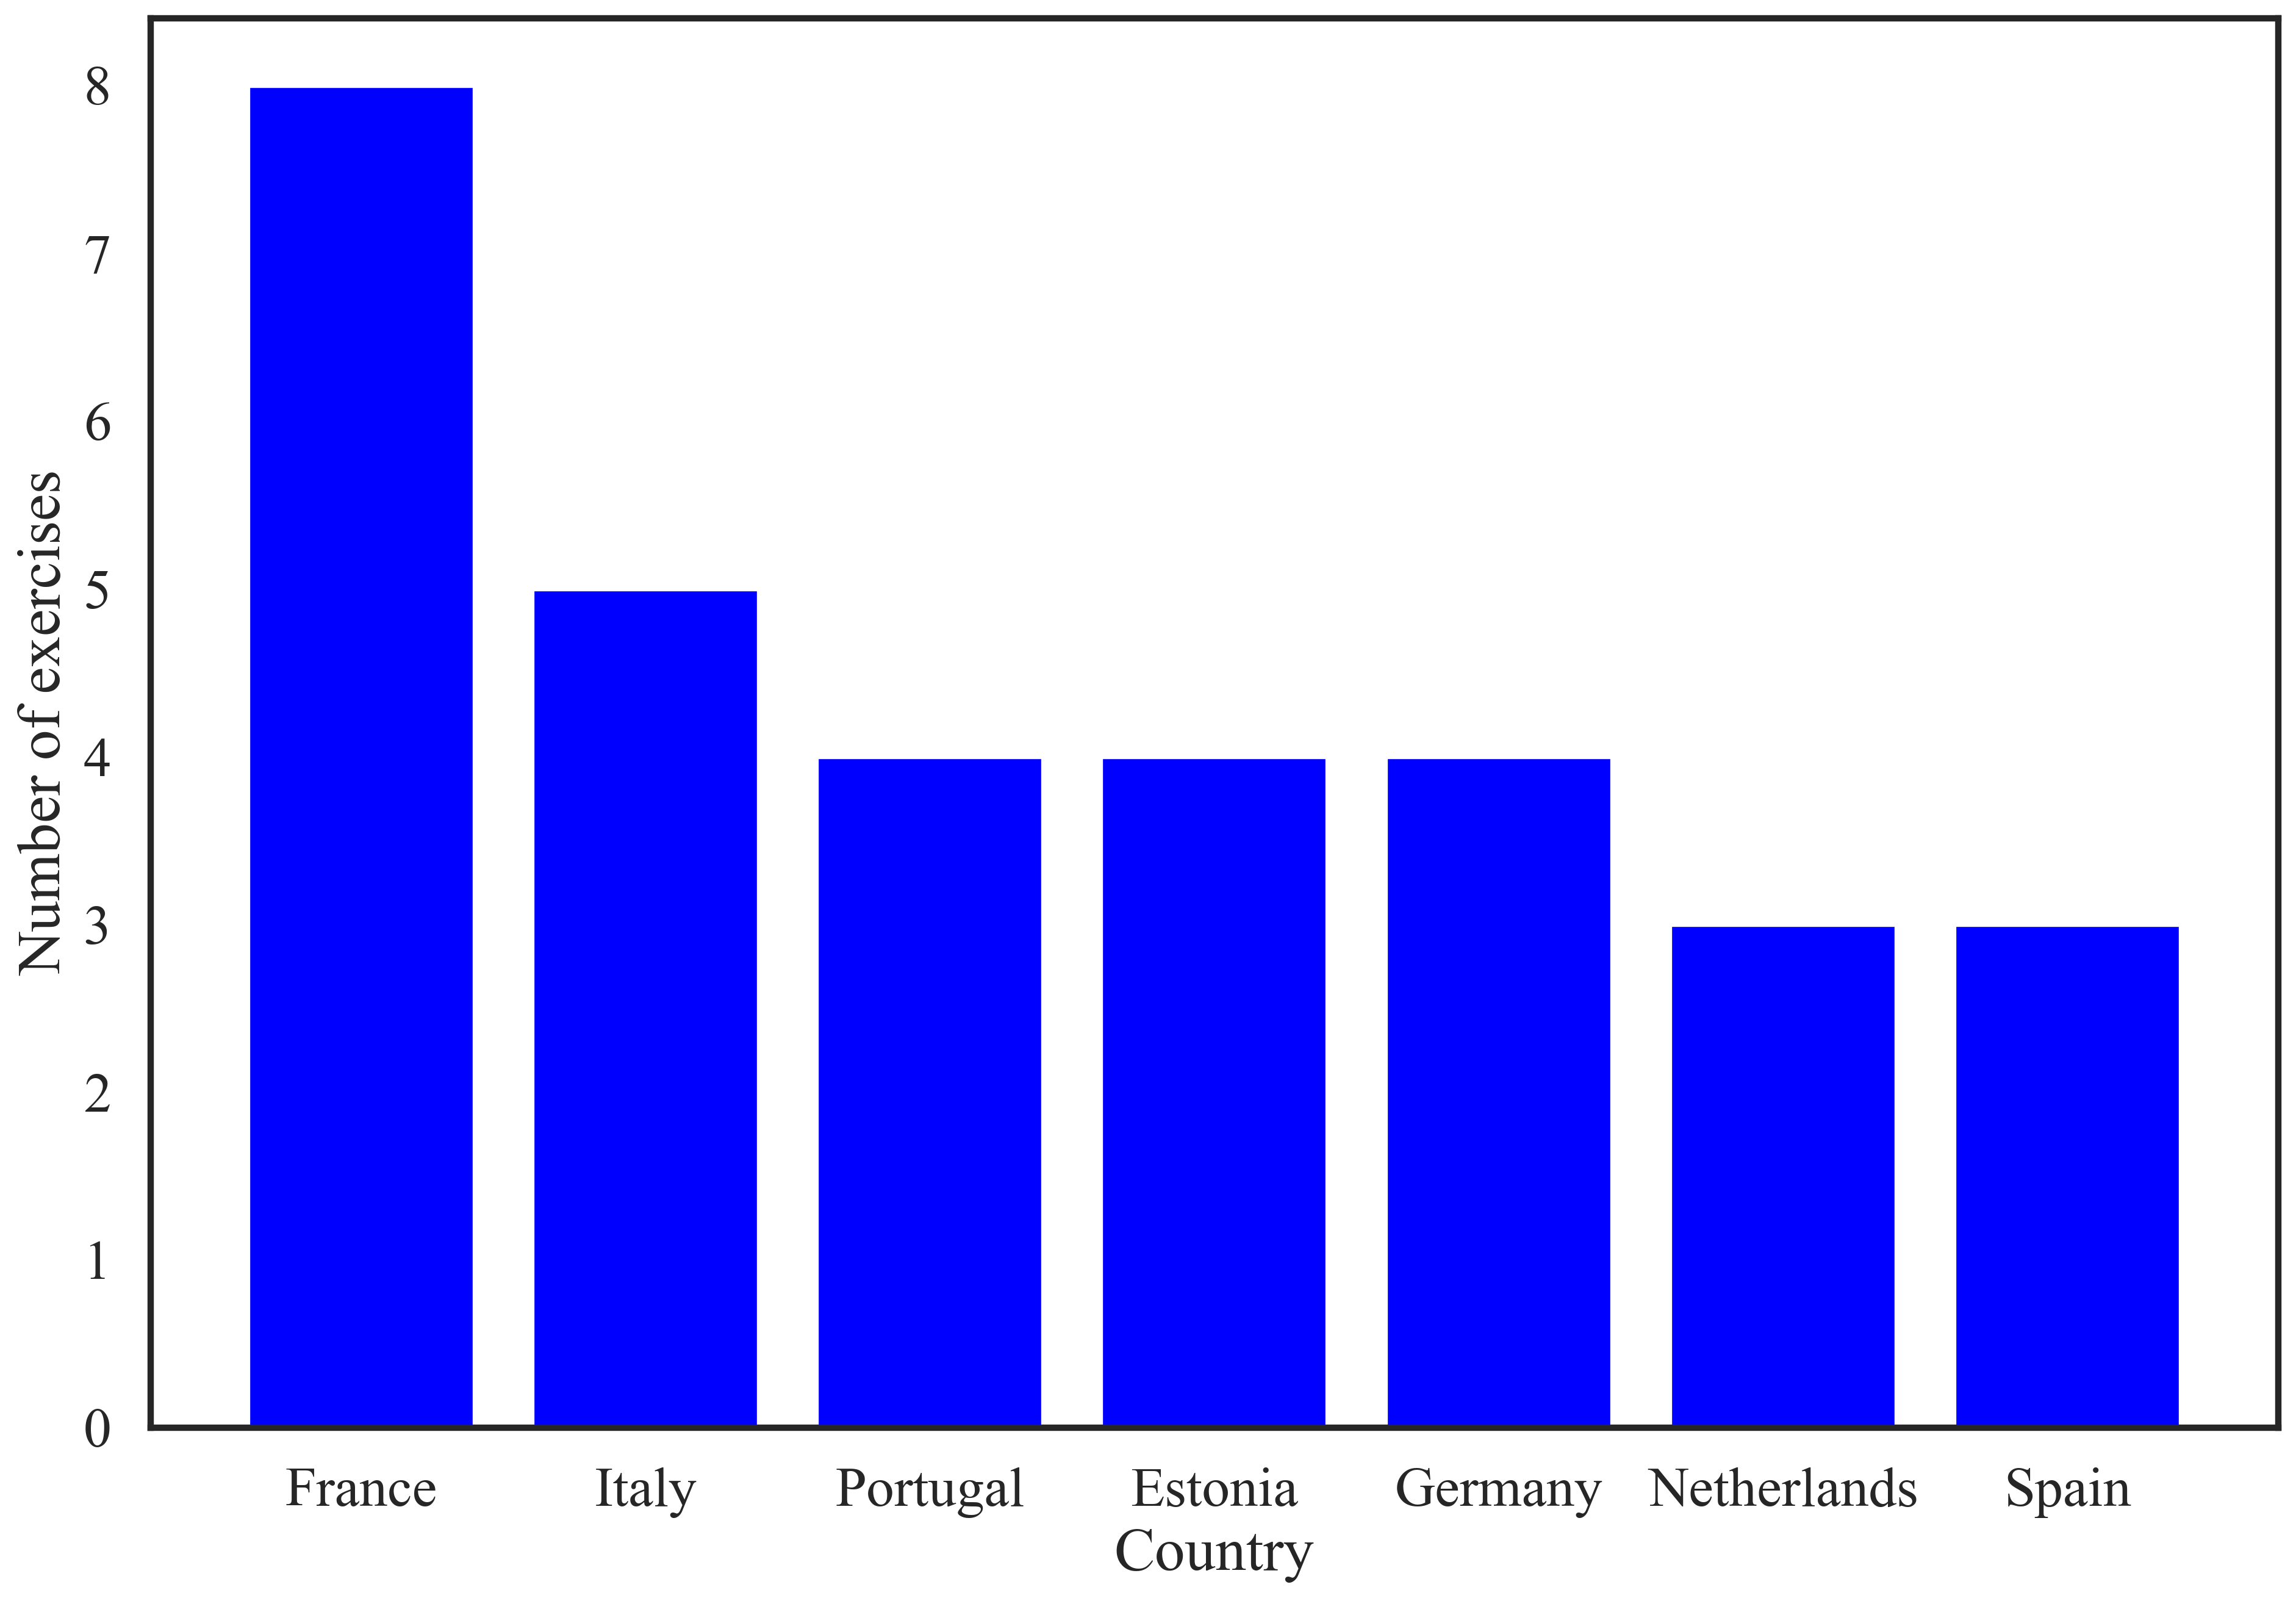
\includegraphics[width=1\textwidth]{Images/cyber_exercises.png}
    \caption{\textit{EU Cyber Projects under PESCO by Country}}
    \source{Source: pesco.europa.eu}
    \label{fig:cyber_exercises}
\end{figure}

Collectively, these PESCO projects represent a concerted effort by the EU to operationalize its cybersecurity objectives, acknowledging the dynamic and multifaceted nature of contemporary cyber threats. The strategic allocation of resources and collaborative approach underscore the EU's commitment to fostering resilience and adaptability in the face of evolving cyber challenges. However, those PESCO missions are just a few examples of missions involved in the cyber domain. The notable involvement of certain countries in PESCO missions signifies a strategic commitment to collaborative defence initiatives within the European Union. France emerges as a particularly active participant, contributing to eight PESCO projects, showcasing a strong dedication to enhancing European cybersecurity capabilities. Italy closely follows with involvement in five projects, further underlining its commitment to cooperative defence efforts. Portugal, Estonia, and Germany each demonstrate notable engagement, contributing to four projects apiece. The Netherlands and Spain are also actively involved, participating in three projects each. This distribution of involvement suggests a core group of nations taking the lead in shaping the direction and success of PESCO missions. This concentrated participation from key member states contributes to the effectiveness and impact of collaborative cybersecurity endeavours within the European Union.

\section{Conclusion}
The willingness of the European Union to become a cyber power and increase its strategic relevance in the international field is evident. However, the understanding of its cyber capabilities is different from analysing other state-actors. Even though the EU is not primarily involved in military security, the cross-sector nature of cyberspace gives the EU the possibility to emerge as a normative cyber power \autocite{wagnsson_2018_normative}. As a normative cyber power, the EU represent a unified member states perspective while guaranteed the coordination of policies and investment in the cyberspace. Whether this coordination and perspective is and will remain coherent in the future, is the crucial aspect that will define the efficacy of the cyber strategy. 




\chapter{Assessing European Preparedness for Cyber Warfare: A Comparative Analysis of France, Estonia, Germany, and the Netherlands}


\section{Introduction}
The selection of Estonia, France, Germany, and the Netherlands for our cyber defence analysis is rooted in their pivotal roles within the European Union's strategic framework, despite embracing diverse approaches to cybersecurity. This strategic diversity spans from Estonia, recognized for its extensive experience as a cyber defender, to the Netherlands, France, and Germany, major players in European Union politics. The inclusion of these nations in our study is driven by their influential positions and distinct cybersecurity strategies, offering a comprehensive spectrum of perspectives within the European landscape.

These countries not only showcase varied cyber defence tactics but also hold strategic significance in the European Union's overarching cybersecurity initiatives. Their diverse approaches, ranging from proactive cyber defence measures to nuanced political engagements, contribute to a comprehensive understanding of cybersecurity challenges and strategies at both regional and international levels. Furthermore, the selection is informed by the wealth of official documents and publicly accessible data available from these nations. 

\begin{figure}[H]
    \centering
    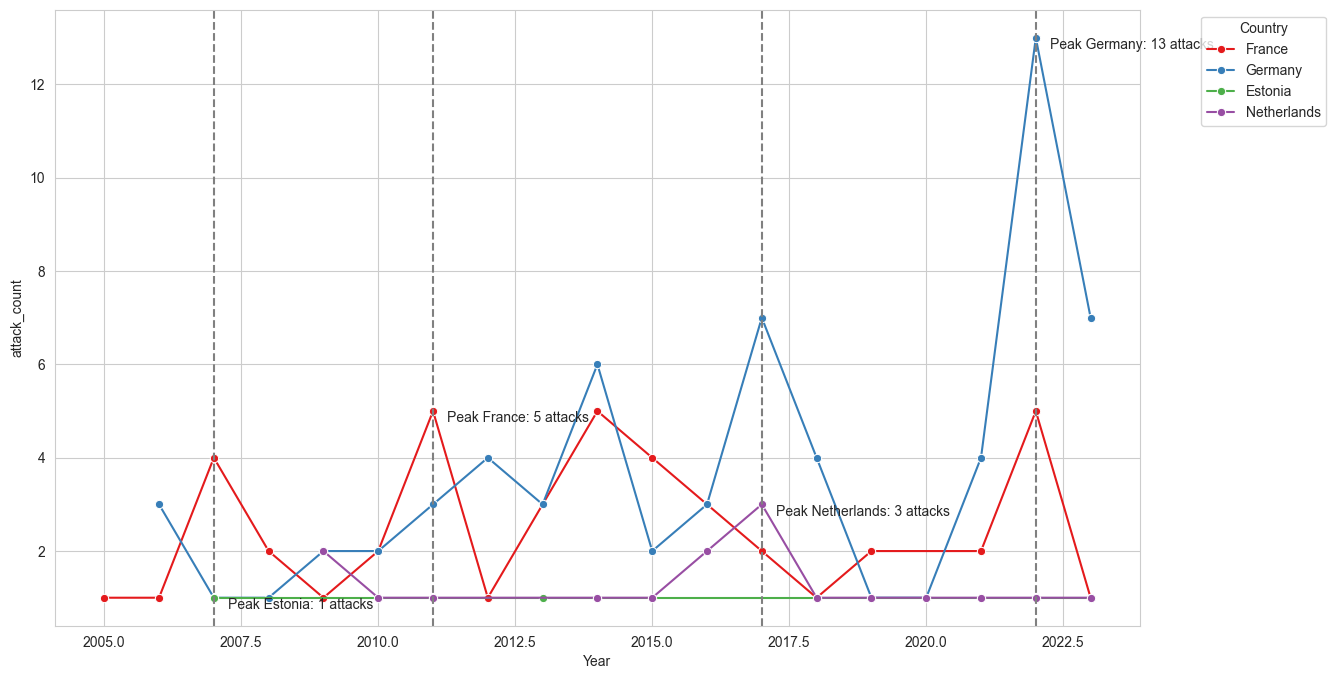
\includegraphics[width=1\textwidth]{Images/attack_countries.png}
    \caption{\textit{Number of State-sponsored cyber operations 2005-2023}}
        \source{Source: \autocite{eurepoc2023}}
    \label{fig:attack_countries}
\end{figure}

The line plot in Figure \ref{fig:attack_countries} depicts the landscape of state-sponsored cyberattacks experienced by the analysed countries. The data was obtained through exploratory data analysis from the EuRepoC dataset, and a table with years and cyberattacks is provided in Appendix \ref{tab:cyberattacks_per_year}.

Germany has encountered more cyber operations than its counterparts, experiencing a significant surge after the war in Ukraine. Germany is considered the most active European country in providing military support to Ukraine, and it holds a crucial position as a political and economic player, not only within the European context but also on the global stage. Furthermore, France follows Germany closely in terms of the number of attacks. The increased frequency of attacks is not directly linked to an inability to counter them but rather to the overall number of attacks, given that attack vectors can have a multiplied effect in a larger and more connected economy.

Estonia and the Netherlands, on the other hand, have faced fewer attacks. Specifically, Estonia has drawn valuable lessons from the 2007 attacks, contributing to an enhancement of its preparedness. Additionally, the smaller size of its economy and state support contribute to a more defensive approach.

Russia has been the most attributed country for cyberattacks in Estonia and Germany, while China is associated with attacks in France and the Netherlands \ref{cod:attacker}.

\begin{figure}[H]
    \centering
        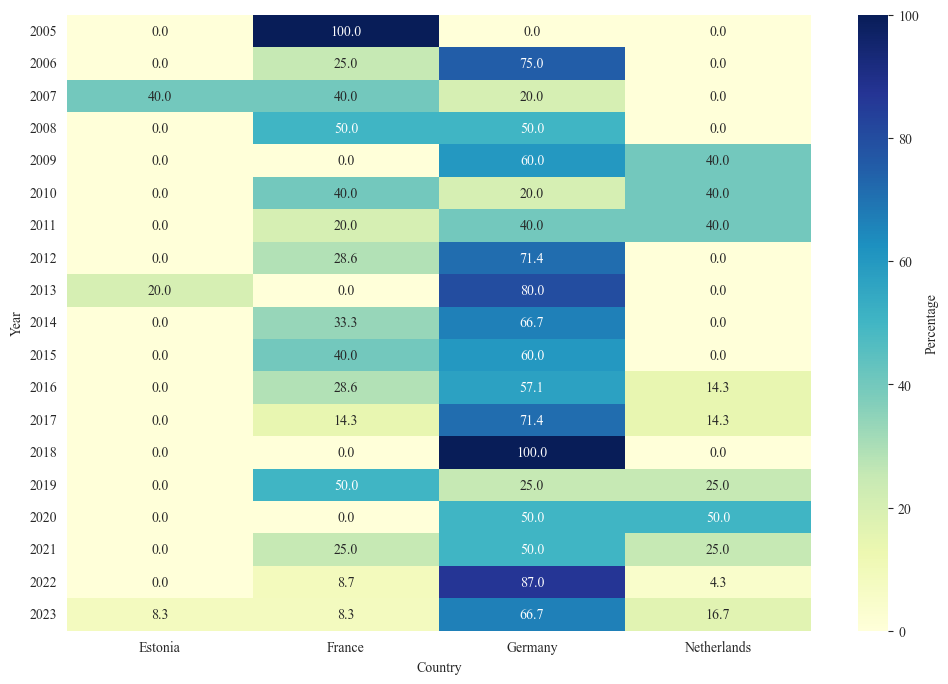
\includegraphics[width=1\textwidth]{Images/disruption.png}
        \caption{\textit{Percentage of disruption after State-sponsored cyber operations 2005-2023}}
        \source{Source: \autocite{eurepoc2023}}
        \label{fig:disruption}
\end{figure}


Furthermore, another analysis has been conducted regarding the disruption caused by the attacks. Mostly, the countries have experienced an improvement over the years, as associated with low disruption in cyberattacks, as depicted in Figure \ref{fig:disruption}. However, it is important to note that Germany has not only encountered a higher number of cyberattacks but also more disruption resulting from them. This highlights the probability of Germany being a crucial target for foreign cyber operations while possessing fewer capabilities to counter them.

Following this overview, the chapter will delve specifically into the cyberstrategies of the analyzed countries, aiming to gain insights into how these nations are influencing changes in cyber strategies after the war in Ukraine and what challenges lie ahead.


\section{France}

This section offers a comprehensive exploration of France's cyber defence strategy, meticulously outlined in the Strategic Review of Cyber Defence \autocite{sgdsn_2018_strategic}. By dissecting key components such as operational chains, governance structures, and specific doctrines, we aim to uncover the interconnected layers that constitute France's resilient stance against evolving cyber threats.

In February 2018, France released a White Paper, signalling a strategic shift in its approach to cyber defence. Beyond a mere enumeration of operational chains and governance bodies, this analysis seeks to unravel the cohesive strategy that guides France's response to the dynamic cyber threat landscape.

France's cyber defence strategy unfolds through four operational chains, each with a distinct role. The Protection Chain, spearheaded by SGDSN and ANSSI, stands as the frontline defence for national security during cyberattacks. Complementing this, the Military Action Chain provides the President with the authority to deploy cyber warfare in the interest of national defence. Simultaneously, the intelligence chain focusses on attribution of cyberattacks, while the judiciary investigation chains involve law enforcement in the aftermath of cyber-related crimes \autocite{sgdsn_2018_strategic, anssi_2022_le}.

\begin{figure}[H]
    \centering
    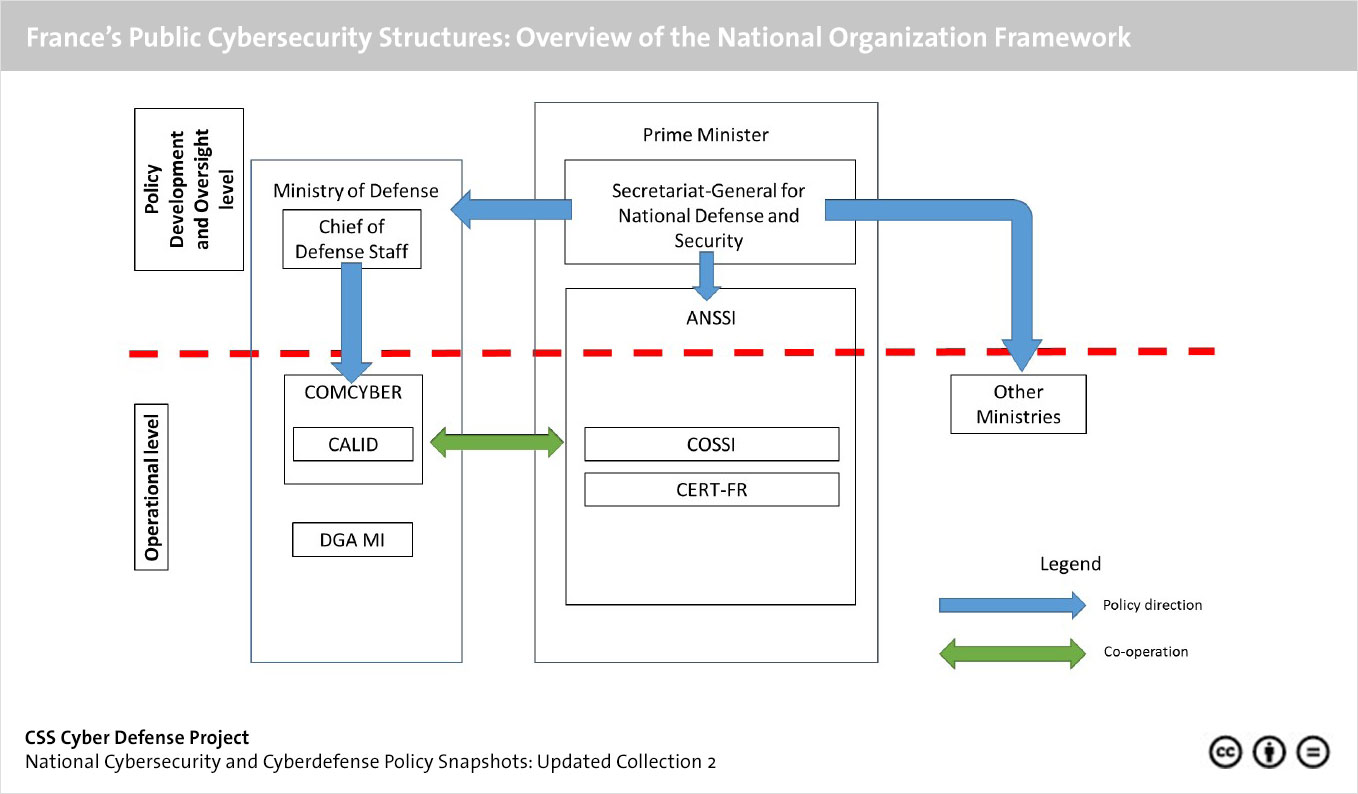
\includegraphics[width=1\textwidth]{Images/france.jpg}
    \caption{\textit{France Cyber Structure}}
        \source{Source: \autocite{sdewar_2018_national}}
    \label{fig:france}
\end{figure}

\textbf{Governance and Crisis Management}: Beyond the operational facets, France has meticulously crafted a governance structure to manage cyber crises. The Cyber Defence Management Committee, the Cyber Defence Steering Committee, and the Cyber Crisis Coordination Centre collectively orchestrate a coordinated response.  Permanent Cyber Posture (PPC) ensures uninterrupted 24/7 defence, reflecting a commitment to proactive cyber defence. This interplay of structures and strategies exemplifies a holistic approach to cyber resilience.

\textbf{Defensive Cyber Warfare Policy (LID)}: The Defensive Cyber Warfare Policy (LID) serves as the linchpin of France's defensive capabilities. Beyond a mere list of missions, LID embodies a strategy of awareness, probability assessment, protection enhancement, detection, reaction, and attribution. The interdependence between these missions showcases a holistic approach to safeguarding national interests. Moreover, the emphasis on collaboration, exemplified by the Network and Information Systems Directive (NIS) and its updated version (NIS2), emphasizes the importance of unified efforts between electronic communication operators, web hosts, and national entities. Local level involvement through coordination forums further cements the idea of a collective defence \autocite{ministredesarmes_2019_politique}.

\textbf{Offensive Cyber Warfare Doctrine (LIO)}: In tandem with defensive measures, France has integrated offensive capabilities within its overall military strategy through the Offensive Cyber Warfare Doctrine (LIO). COMCYBER, operating under the Chief of Staff of the Armed Forces, oversees the orchestration of LIO. By acknowledging the necessity for political, legal, and military risk evaluations, France strikes a delicate balance between secrecy and transparency. The democratic nature of the state guides decisions on the disclosure of LIO actions \autocite{ministredesarmes_2019_lments}.

\textbf{Influence Computer Control (L2I)}: Expanding beyond national borders, France recognizes the importance of information warfare through the Influence Computer Control (L2I). Executed by CYBERCOM, L2I operations aim to detect and counter information attacks, gather intelligence, and engage in deception operations. Challenges, such as the investment in human resources, are met head-on through the Military Program Law 2019-2025, allocating resources for cyber fighters and acknowledging the financial commitment needed \autocite{ministredesarmes_2021_lments}.

France identifies private companies or public bodies that are of vital importance. The \textit{Secteur d'activité d'importance vital} applies to these, a provision which raises the level of security in the event of an attack, including cyberattacks. Due to the increase in cyberattacks, the provision has been transformed specifically for vital information systems (making information systems a separate category of cyber infrastructure). To date, more than 200 entities have been labelled as such with the obligation to notify any incident, as well as apply more stringent crisis prevention and management measures \autocite{anssi_2022_le}.

In conclusion, France's cyber defence strategy is a tapestry woven with interconnected threads, each playing a crucial role in ensuring national cybersecurity. By delving beyond the surface enumeration of strategies, this analysis unravels the symbiotic relationship between operational chains, governance structures, and specific doctrines. In an era of evolving cyber threats, France's adaptive and integrated approach stands as a model for nations navigating the complex landscape of digital security. Furthermore, France has increased its awareness and cyber capabilities even before the War in Ukraine, anticipating strategies on the involvement of public sector in the cyber defence and the use of offensive attacks in their doctrine. However, no public available information for the integration of cyber and kinetic weapons were found. 

\section{Estonia}
Estonia experiences with cyberattacks has shaped not only its own strategy but also became a successful model of how to exploit security vulnerabilities to improve its readiness to counter future attacks. After 2007, Estonia have developed a multifaced cyber strategy, an outcome from a continuous learning and development of proactive defence measures. 

\textbf{National Security concerns} Unlike the other countries analysed in this dissertation, Estonia is more familiar with a real threat that combines kinetic and cyber operations from non-state actors (supported from Russia). In this regard, the National Security Concept published in 2017 highlight that Estonia applies measures to guarantee the digital continuity of the state even in situations where it has lost the control over its territory \autocite[16]{republicofestonia_2017_national}. For a small state like Estonia, the synergy between the private sector, the civil society and the State becomes a priority.  

As well as in the previous analysis, the main challenge that Estonia must tackle regards the skill and specialization. Even the flexibility of being a small country helps professionals to connect with each other and create communities which are valuable in the cyber domain, this approach to the crisis management could not be sustainable due to increase complex of technology risks.  

\textbf{International Cooperation \& exercises} Estonia is actively involved in the international cooperation in the cyber domain. It hosts the Cooperative Cyber Defence Centre of Excellence (CCDCOE), a NATO-accredited centre for cybersecurity and cyber defence. In fact, Tallinn CCDCOE hosts the most important NATO cyber exercises, such as the Cyber Coalition and Locked Shields. The alignment with allied military presence, particularly NATO's Enhanced Forward Presence (eFP), underscores the need for evolving cooperation mechanisms and procedures to collectively address cyber threats. Estonia aims to establish a comprehensive approach, encompassing political, legal, and technical dimensions, to attribute cyber-attacks, participate in deterrence efforts, and collaborate with like-minded countries in cyber defence frameworks \autocite{ministryofeconomicaffairsandcommunication_2019_cybersecurity}. 

The small Baltic country has also bilateral cyber exercise such as Baltic Blitz 23 with United Stated, as well as joint defensive operations with the USCYBERCOM\footnote{ Information about this operation were published by the US Cyber Command on their website: https://www.cybercom.mil/Media/News/Article/2433245/hunt-forward-estonia-estonia-us-strengthen-partnership-in-cyber-domain-with-joi/}. While Estonia official document do not mention the cyber offensive capabilities of their military, the Baltic State has been a central player in hosting NATO Crossed Swords, a redteamming exercise with the aim to explore the kinetic-cyber synergies in a wartime scenario \footnote{ Even if exercises like that are under exceptional secrecy, local media offers useful insights: https://news.err.ee/1608427058/offensive-cyber-operations-exercise-kicks-off-in-estonia}. 

\begin{figure}[H]
    \centering
    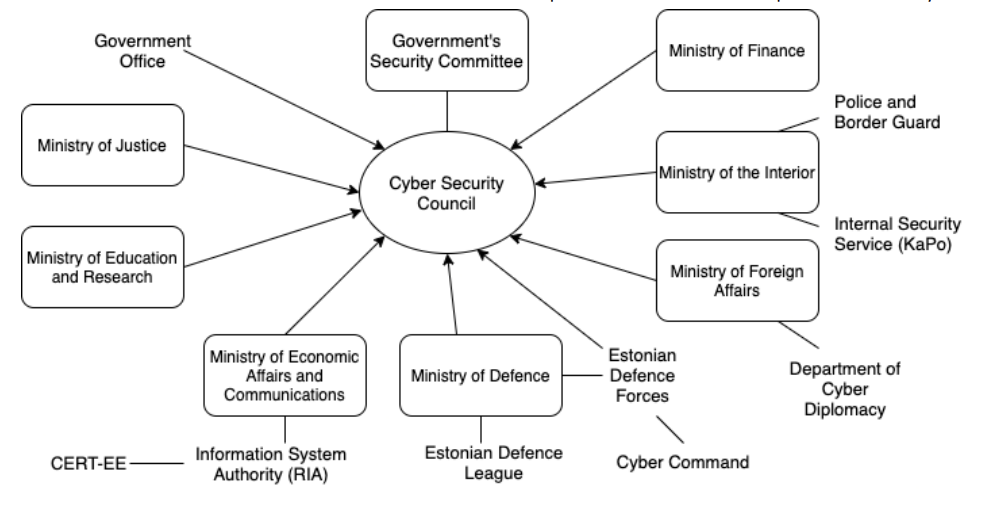
\includegraphics[width=1\textwidth]{Images/estonia.png}
    \caption{\textit{Estonia Cyber Structure}}
        \source{Source: \autocite{kohler_2020_cyberdefense}}
    \label{fig:estonia}
\end{figure}

\textbf{Cyber Military structure} From the military perspective, the Cyber Command, which become operation in 2018, have the task to carry out cyber operations and to provide cyber defence. The Cyber Command subdivisions include \autocite{defenceforces_2023_cyber}: 
\begin{itemize}
    \item ICT centre: develop the defence architecture of military forces, as well as coordinating the development in the technology domain. 
    \item Cyber Information Operation Centre: prepare the reserve units and active planning of cyber operations and defence.
\end{itemize}

Estonia represents a unique case in which a civil cyber army is officially recognized as part of the Estonian Armed Forces. The country's cyber civil defence force, which is integrated into the Estonian Defence League, is dedicated to enhancing national cyber resilience. Members of this unit typically comprise IT professionals, programmers, and individuals possessing expertise in cybersecurity. The cooperation between civil society and the state is palpable in this framework. By involving IT experts and cybersecurity specialists from outside traditional military establishments, Estonia fortifies the bond between the government and the public, thereby cultivating a shared responsibility for national cybersecurity.

Estonia embrace deterrence by denial in the cyberspace \autocite{oh_2019_exploring}. The aim is to make it difficult for attackers to achieve their objectives, thereby dissuading them from attempting cyberattacks in the first place. 

\textbf{Protection of Critical Infrastructure} For what regards the protection of critical information infrastructure, the Information System Authority (RIA) is the competent authority which encompass the cyber crisis management. Additionally, RIA works with state authorities and businesses that provide essential services to coordinate efforts to avoid and handle cyber emergencies. It also collaborates on civilian-military cyber initiatives with the Defence Forces and Defence League. Moreover, RIA coordinates the national response to significant cyber incidents, which are defined as incidents that jeopardize or negatively impact system security, in compliance with the Emergency Act. Through incident prevention, preparedness planning, and incident response coordination, RIA maintains a state of readiness by utilizing strategies like legislative advancements, security officer network management, and other training efforts. In order to prepare for large-scale cyber incidents, RIA's Incident Response Department regularly conducts risk analyses to evaluate the likelihood and consequences of such events. Depending on the type and extent of the emergency, this preparation may involve working with other cybersecurity departments and pertinent authorities listed in the Emergency Response Plan, such as the Cyber Unit of the Estonian Defence League \autocite{informationsystemauthority_2022_cyber}

Estonia plays an important role in the cyber diplomacy. The 2007 Russian cyberattacks served as a turning point, prompting Estonia to intensify its efforts in cyber diplomacy. In 2018, it appointed its first ambassador-at-large for cybersecurity, and the following year, a dedicated department was established to lead the country's cyber diplomacy initiatives \autocite{theinternationalinstituteforstrategicstudies_2023_cyber}.  



In summary, Estonia's response to cyber threats stands as a resilient model shaped by its experiences, particularly the impactful cyberattacks in 2007. This multifaceted strategy reflects a continuous commitment to learning and proactive defence. Unlike its counterparts, Estonia faces a tangible threat, blending kinetic and cyber operations from non-state actors, necessitating measures to ensure digital continuity even in the absence of territorial control.

\section{Germany}

Germany plays a central role in both economic and political spheres within the European Union. While its defence and civil industry are robust, the cybersecurity and cyberdefence sectors are still undergoing continuous development. This evolution is taking place under a centralized structure, with key responsibilities allocated to the Ministry of Interior and the Ministry of Defence. The War in Ukraine caused a sharp strategic position on boosting its military capabilities, with €100 billion, 21 of which dedicated to the improvement of communication and cyber capabilities. 

\begin{figure}[H]
    \centering
    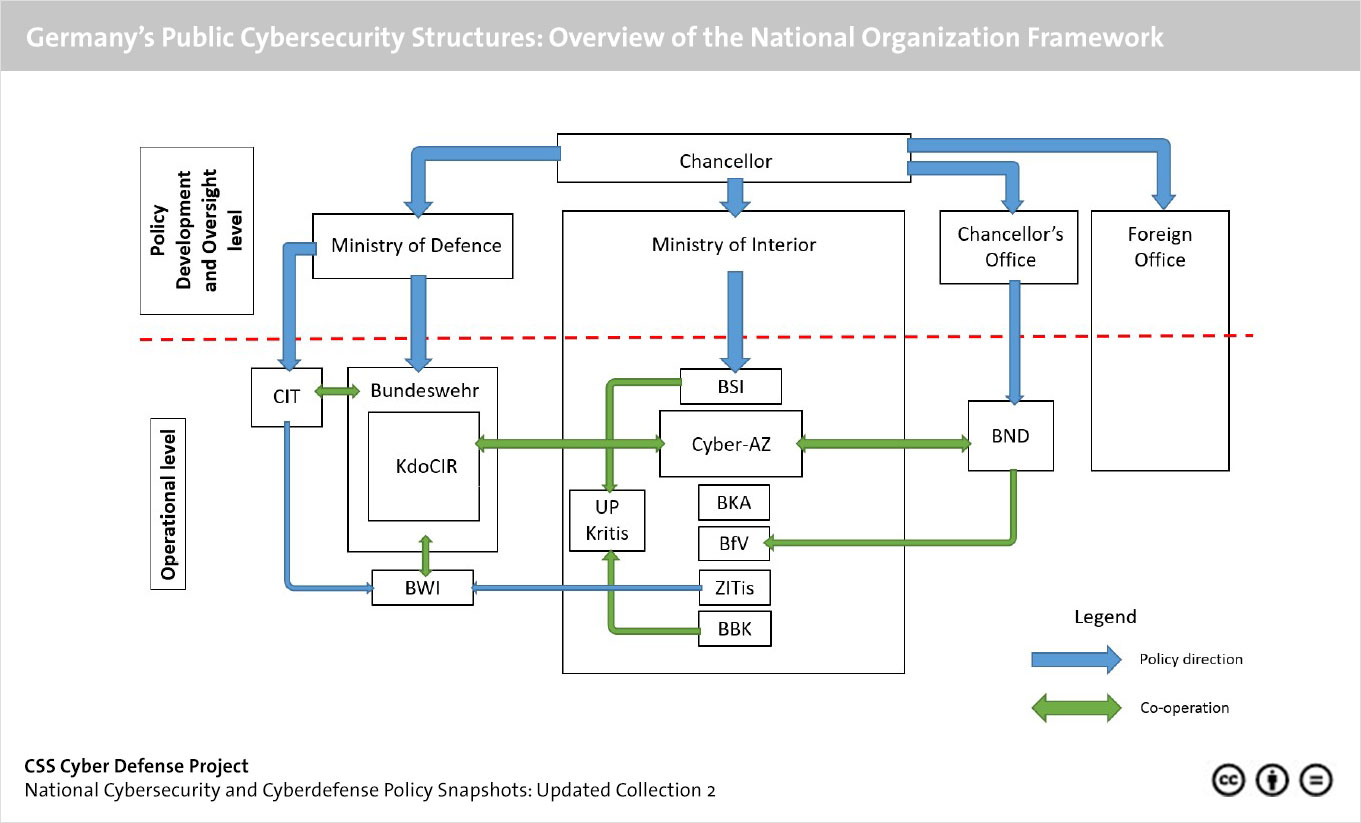
\includegraphics[width=1\textwidth]{Images/germany.jpg}
    \caption{\textit{Germany Cyber Structure}}
        \source{Source: \autocite{sdewar_2018_national}}
    \label{fig:germany}
\end{figure}

\textbf{Germany Cyber Structure} Germany's cyber-security architecture is complex, with its governance distributed between different government entities. The Federal Ministry of the Interior (BMI) controls the police forces and domestic intelligence service. Furthermore, within the Central Office for Information Technology in the Security Sector centralise the government governance role regarding cyber activities, while coordinating with the National Cyber Security Strategy (NCSS). On the other hand, the Federal Office for Information Security (BSI) sets best practices, guidelines and standards for the cybersecurity measures. \autocite{theinternationalinstituteforstrategicstudies_2023_cyber, federalministryoftheinteriorbuildingandcommunity_2021_cyber}

At the national level, the National Cyber Security Council coordinates the federal government's cyber-security policy and fosters collaboration between the public and private sectors. The Ministry of Defence (BMVg) is responsible for protecting its systems and engaging in cyber-security, including offensive cyber operations. The CIT focuses on acquiring, using, and protecting the IT infrastructure of the BMVg, the nationalized company BWI, and the Bundeswehr. Its role is to streamline responsibilities, promote technological development, and harmonize soft- and hardware capabilities. In addition, the KdoCIR operates independently of traditional military branches and is tasked with protecting critical infrastructure, conducting computer network operations, recognizing propaganda and disinformation, participating in opinion-making, and compiling military and cyber intelligence. The KdoCIR comprises two main pillars: the Strategic Reconnaissance Command (KdoStratAufkl) and IT Command of the Bundeswehr (KdoITBw). The former focuses on intelligence information management and reconnaissance in cyberspace, while the latter is responsible for IT-system operations, cybersecurity, and IT evaluation. Germany represents a forward position toward a structured cyber defense within the military domain and considered the best computer forensic expert from the NATO members \autocite{leinhos_2020_cyber}. 

The Federal Intelligence Service (BND) is Germany's primary foreign intelligence agency, engaging in cyber-intelligence operations with a focus on signals intelligence. The BND operates under a unique legal regime, conducting cyber espionage and intercepting communications. The Federal Office for the Protection of the Constitution (BfV) handles domestic intelligence, including some cyber-security and cyber-espionage functions. The Military Counter-Intelligence Service defends against attacks on the German armed forces. \autocite{theinternationalinstituteforstrategicstudies_2023_cyber, federalministryoftheinteriorbuildingandcommunity_2021_cyber}

Germany has set up a Federal Agency for Innovation in Cybersecurity, denominated \textit{Cyberagentur}, with the aim to speed up the innovation in this sector. Their strategy focuses on the development of AI systems for cybersecurity as well as applications of cryptography and quantum computing \footnote{For more information, please consult the following document: https://www.cyberagentur.de/wp-content/uploads/2023/11/Strategie-2022-2025-Internet.pdf}. 

\textbf{Offensive or Defensive capabilities?} Germany is positioned towards an active cyber defence role \autocite{federalministryoftheinteriorbuildingandcommunity_2021_cyber}. However, the German Basic Law constrains the intervention from the Bundeswehr in response to cyberattacks or their attribution, which is considered a responsibility of law enforcement agencies and intelligence services \autocite{leinhos_2020_cyber}. The defence position is focused on protecting state secret and Bundeswehr from cyber espionage and sabotage \autocite{federalministryoftheinteriorbuildingandcommunity_2021_cyber, thefederalgovernmentofgermany_2023_robust}. However, clear strategy on cyber defence from the military perspective, as well as the cyber \& kinetic integration. A critical position for strategic country such as Germany to not be ready (at least from regulatory and public strategic perspective) to have an offensive and defensive cyberstrategy applied to military domain. 

Germany opposes to the offensive cyber capabilities (the so called \textit{hackback} or preventive attack). Its position is less exposed to uncontrolled effect of offensive actions, and it is directly linked with the attribution issues that constitutes an obstacle in the definition of offensive cyber operations towards State actors \footnote{Public announcement have confirmed this position: https://www.euractiv.com/section/cybersecurity/news/german-national-security-strategy-leaves-out-cyber-counter-attacks/}.

\textbf{Protection of Critical Infrastructure} The National Cyber Response Centre have set reconnaissance and early warnings capabilities to promote situational awareness while involving stakeholders to contribute to them (national security strategy). Critical infrastructure and information ones are regulated through the \textit{National Strategy for the Protection of Critical Infrastructures} \autocite{federalofficeforinformationsecurity_2022_up} and \textit{National Plan for the Protection of Information Infrastructure}s (NPSI) respectively. The Cybersecurity strategy stress out the need to replace reactive measure with proactive ones. A problem that emerges on this page is linked to the voluntary nature of strategic entities in participating in the exchange of information, which can be fundamental for preparing for cyberattacks. On the other side, concerns appear about the European inability to guarantee competition at an institutional information level (see 5G and the smartphone market) with Asia and the US, which have built an oligopoly. This negatively affects the ability to guarantee the security of information networks not only in Germany but also in Europe. The German government is pursuing an enhanced cybersecurity framework by fostering collaboration between public sector, research community, private companies and civil society. This collaboration is, and it will be possible through projects like UP KRITIS and the National Pact on Cybersecurity. The outcomes expected are just not related to improving cyber measures but also facilitate information and skills exchange between the vertical and horizontal levels \autocite{federalofficeforinformationsecurity_2022_up, federalministryoftheinteriorbuildingandcommunity_2021_cyber, thefederalgovernmentofgermany_2023_robust}.

\textbf{Intelligence} Germany has stressed out that the settlement of preventive measures it would be possible only through intelligence gathering. This task is delegated to the Federal Office of Military Counter-intelligence (BAMAD), created to acquire information about cyber threats, understating motives, capabilities and attack vectors to prepare the victims. The work of the new counter-intelligence subdivision goes along with the cooperation with other federal intelligence agencies and the private sector \autocite{theinternationalinstituteforstrategicstudies_2023_cyber}. 

\textbf{Challenges ahead} As the other countries, Germany faces a critical challenge in recruiting talents in the cybersecurity domain \autocite{thefederalgovernmentofgermany_2023_robust, leinhos_2020_cyber}. In this regard, the cyber cluster at the \textit{Universität der Bundeswehr München} in Munich not only carries out research but also provides basic, advanced and further training for officers and Federal Government employees, with a focus on cybersecurity \autocite[25]{federalministryoftheinteriorbuildingandcommunity_2021_cyber}. Another issue regards the IT procurement and innovation of both terminals and infrastructure. Some step-forwards have been made with the modernization of C2 capabilities, however, failure to update technological equipment would create surface attacks and undermine the effectiveness of the military structure itself. Germany underlines in both its cybersecurity strategy and its strategic concept that security in the cyberspace (as in other areas) is possible to achieve only with cooperation with European and International partners \autocite[22]{federalministryoftheinteriorbuildingandcommunity_2021_cyber}. In particular, Germany emphasizes the role of the European Union in achieving the digital sovereignty, streaming research, procurement new technologies commissioning \autocite[23]{federalministryoftheinteriorbuildingandcommunity_2021_cyber}. In addition. Germany has set the objective to establish a consistent European regulatory framework for businesses in the cybersecurity sector, addressing the current inconsistencies and lack of binding standards at the national and international levels\autocite{federalministryoftheinteriorbuildingandcommunity_2021_cyber}.  

\section{Netherlands}

\textbf{Netherlands Cyber Structure} The cybersecurity infrastructure of the Netherlands reflects a robust and multifaceted approach, encompassing a diverse set of organizations and initiatives. Central to this framework is the Dutch National Cyber Security Center (NCSC-NL), operating under the Ministry of Justice & Security and the National Coordinator for Security and Counterterrorism (NCTV). Functioning as the national Computer Emergency Response Team (CERT), NCSC-NL plays a pivotal role in safeguarding critical infrastructure and assisting central government entities. Additionally, the Digital Trust Center (DTC) engages in a three-year program aimed at securing digital businesses, particularly small to medium-sized enterprises. The collaboration between these entities underscores a commitment to a safe and resilient digital society. Furthermore, the Cyber Security Council (CSR) operates as a unique private-public partnership, providing strategic guidance to the Dutch Cabinet on cybersecurity matters and fostering awareness in the private sector. The Ministry of Defence (MoD) adopts an active defence stance, investing in capabilities ranging from information capacity to military support for civilian authorities. The inclusion of entities such as DefCERT and the Defence Cyber Command underscores the comprehensive nature of the Dutch cyber defence strategy \autocite{sdewar_2018_national, theinternationalinstituteforstrategicstudies_2023_cyber}.

\begin{figure}[H]
    \centering
    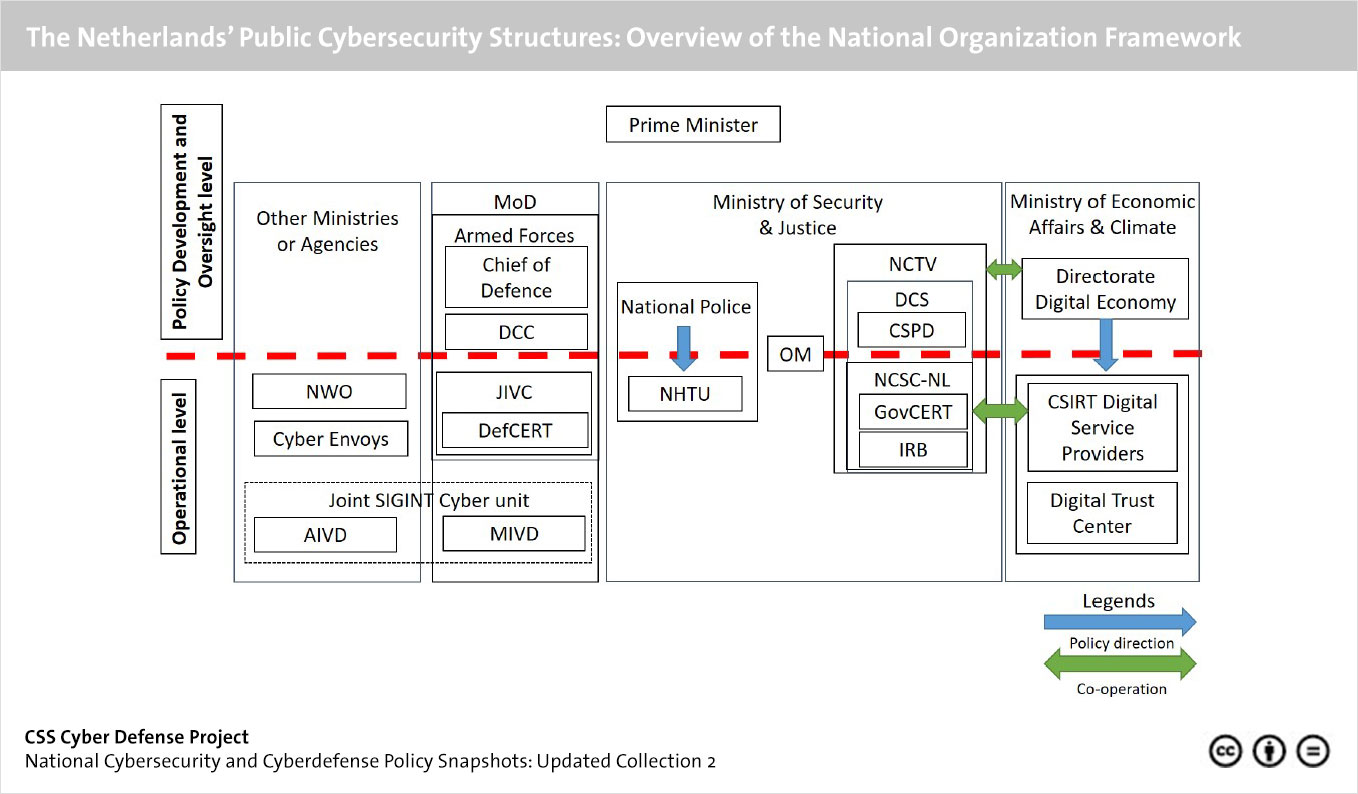
\includegraphics[width=1\textwidth]{Images/netherlands.jpg}
    \caption{\textit{Netherlands Cyber Structure}}
        \source{Source: \autocite{sdewar_2018_national}}
    \label{fig:netherlands}
\end{figure}

\textbf{Public-Private collaboration} Due to the interconnection between digital services and infrastructure in both the public and private spheres, the Netherlands has established the Nationwide Network of Cybersecurity Partnership (LDS), which will be further developed in the future. The aim of this entity is to facilitate and improve the sharing of information \autocite{ministryofjusticeandsecurity_2022_netherlands}. Another important step toward a more secure infrastructure and cyber environment involves the need to apply the secure-by-design principle to both hardware and software assets. EU regulations, such as the Cyber Resilience Act and Cybersecurity Act, will impose strict rules to guarantee the security of ICT products throughout their lifecycle. Furthermore, the Netherlands has prepared a National Plan for Digital Incidents to effectively respond to potential cyber threats and crises in the digital domain. This comprehensive plan outlines the necessary strategies and actions to be taken in the event of a digital incident, ensuring a coordinated and swift response. 

\textbf{Intelligence gathering} The Netherlands has developed intelligence gathering capabilities. Important information is regularly exchanged with its partners, aligned with the proposed objectives. Additionally, the Defence Intelligence and Security Service (DISS) plays a crucial role in providing intelligence on cyber threats to various entities, including Defence, DefCERT, the Public Prosecution Service, the National Cyber Security Centre (NCSC), and the private sector. The DISS contributes to the National Detection Network (NDN) to detect and respond to cyber espionage and sabotage, collaborating with other organizations. The DISS's intelligence forms the basis for offensive cyber capabilities and allows for proactive defence measures. Furthermore, increasing intelligence capabilities will enable the Netherlands to assess the attribution of the attack more precisely, making the country less attractive for attacks \autocite{theinternationalinstituteforstrategicstudies_2023_cyber, ministryofdefence_2018_defence}.

\textbf{Offensive \& Defensive capabilities} In the context of Cyberstrategy 2022-2028, it is claimed that the government possesses both offensive and defensive cyber capabilities, demonstrating effectiveness in both peacetime and wartime scenarios \autocite[38]{ministryofjusticeandsecurity_2022_netherlands}. While the specific details of these capabilities remain undisclosed for security reasons, the document provides insight into the overarching doctrine and strategies that could be employed. Notably, the document acknowledges the potential utilisation of criminal and non-criminal assets to counteract and disrupt cyberattackers, presenting a diplomatic stance on the Netherlands' possession and potential deployment of offensive (destructive) cyber capabilities. The Netherlands has been developing offensive cyber capabilities, reflecting a proactive approach to countering cyber threats. The International Institute of Strategic Studies highlights joint efforts by DCC and MIVD to develop these capabilities, including involvement in \textit{ defend forward} strategies, where foreign malware is actively addressed to prevent potential attacks on national security \autocite{theinternationalinstituteforstrategicstudies_2023_cyber}. However, the National law framework does not allow the application of those capabilities in peacetime. 

A significant development related to this stance occurred on December 2, 2022, when the cabinet introduced a bill titled \textit{Temporary law on AIVD and MIVD investigations into countries with an offensive cyber programme} to the House of Representatives. This legislative initiative is a direct response to operational challenges faced by the General Intelligence and Security Service (AIVD) and the Military Intelligence and Security Service (MIVD) in conducting investigations into cyber threats originating from state actors \autocite{nationalgovernmentofthenetherlands_2023_internationale}. This legislative proposal signifies the government's commitment to addressing operational bottlenecks and underscores the evolving nature of its cyber defence and offence strategies in the face of emerging threats.

From an organisational perspective, the Netherlands is promoting the establishment of Joint Cyber Mission Teams. Their role will expedite the integration of cyber weapons in a wartime scenario. The teams will be made up of personnel with diverse experience, bringing together individuals from DISS and the armed forces. This collaborative approach recognises the complementary nature of the knowledge and skills required for effective intelligence and military operations in the cyber domain. To enhance transparency and awareness of cyber operationalisation in military missions, Article 100 of the Constitution will be updated with additional statements regarding the cyber domain. The deterrence strategy is not only based on the denial effect through proactive defence, but also with the possibility of using cyber military means to respond to the attacker (known as deterrence by punishment). 

\textbf{Education & Investments} The government's strategic priorities to enhance cybersecurity awareness, education, and expertise are integral to the Cybersecurity Strategy for the 2022-2028 period. Recognising the shared responsibility for digital product security, the government aims to increase awareness among the public and SMEs through targeted information campaigns. To foster a cyber-resilient future, the curriculum for primary and secondary education will include core objectives on cybersecurity skills. The collaboration extends to the labour market, where the government is working with educational institutions and the business community to implement upskilling and reskilling programs. Investments in higher professional education, specifically in the sciences and cybersecurity, focus on increasing admission, reducing dropout rates, facilitating lateral entry, and ensuring a smooth transition to the labour market. This comprehensive approach reflects the government's commitment to building a digitally literate and secure society. Furthermore, the government invested €111 million in cyber resilience, involving the strengthening of critical infrastructure, intelligence agencies, and the improvement of both defence cyber capabilities and an increase in the number of cyber diplomats \autocite{nationalgovernmentofthenetherlands_2023_internationale}. Like other countries analysed, the cybersecurity labour market remains a critical requirement to implement a coherent and efficient cyberstrategy.

\textbf{Cyber-Kinetic Integration} The Netherlands is contributing to the development and implementation of the integration of cyber weapons in NATO missions \autocite{ministryofdefence_2018_defence} Firstly, the country is integrating its IT systems within the Defence organization, encompassing management, command, sensor, and weapon systems. The integration has dual outcomes: on one side, it increases the attack vectors and makes the infrastructure more vulnerable. Yet, on the other hand, it provides a strategic advantage by creating a unified and synchronized approach to military operations. The establishment of a cyber defence command \autocite{theinternationalinstituteforstrategicstudies_2023_cyber} highlights the importance that the Netherlands places on cybersecurity in military affairs.  

\textbf{Cyber Diplomacy} The Netherlands has been a pioneer in applying diplomatic responses to cyberattacks. In accordance with the EU Cyber Diplomacy Toolbox, the country not only responds with sanctions and public declarations against state actors behind cyberattacks, but also counters influence operations actively using cyberattacks and social engineering to shape public opinion, a situation known as hybrid wars. For this reason, the Netherlands strongly believes in the creation of international and European political alliances to counter these threats. In fact, European tools such as the Hybrid Toolbox and the Foreign Information Manipulation and Interference Toolbox, despite their independent nature, can strengthen connections, making it possible to act more effectively and combat fragmentation \autocite{nationalgovernmentofthenetherlands_2023_internationale}.

\newpage

\section{Discussion}
France, Estonia, Germany, and the Netherlands are well qualified and equipped countries to counter cyberattacks, even in emergencies and crises such as war. As advanced and technology-driven economies, the expectation was not to find a lower level than the cases observed in Ukraine, but rather to determine if and how their strategies encompass the risks that we have identified as lessons to be learnt from the war in Ukraine.

The results were twofold. When analysing public documents, it is evident that these countries are structurally prepared and pay specific attention to their IT and critical infrastructure. They also emphasize the role of deterrence and political alliances through the European Union, NATO, and international fora. However, limited information was available regarding the integration of cyber capabilities into military missions.

\begin{figure}[H]
    \centering
    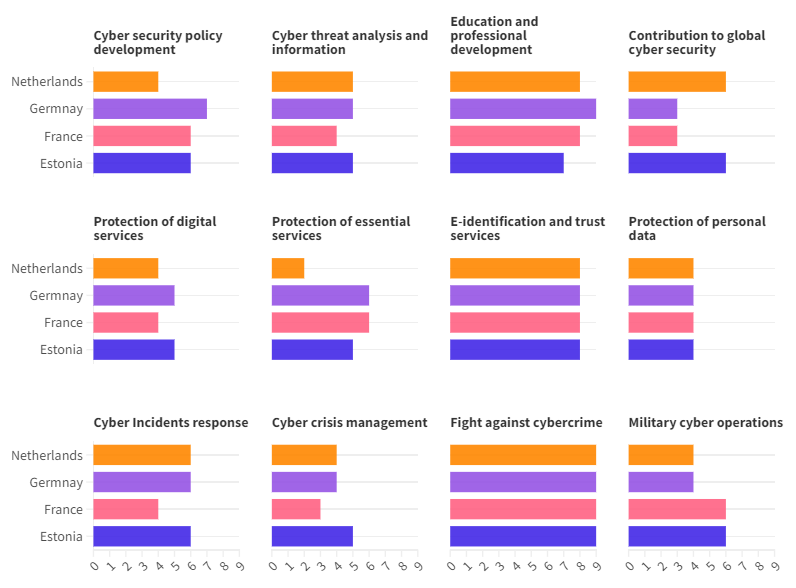
\includegraphics[width=1\textwidth]{Images/ncsi_index.png}
    \caption{\textit{National Cyber Security Index Comparison}}
        \source{Source: \autocite{egovernmentacademy_2023_ncsi}, Author's representation}
    \label{fig:ncsi_index}
\end{figure}

\newpage
\textbf{The National Cyber Security Index}
The Figure \ref{fig:ncsi_index} confirms the analysis performed. Estonia emerges as the leading country in overall cybersecurity, scoring 93.51 out of 100. This is attributed to its robust cybersecurity policy development, high-level cyber threat analysis, and information sharing capabilities. Germany follows closely with a score of 90.91, showcasing strengths in education, professional development, and global contributions to cybersecurity. France, with a score of 84.42, demonstrates a solid foundation in cybersecurity policy and global contribution but lags in some areas like cyber crisis management. The Netherlands, scoring 83.12, excels in education and professional development but faces challenges in the protection of essential services and e-identification. However, the methodology used for computing National Cyber Security Index have issues that have been addressed for the post September 2023 analysis. Similar results have been found with the National Cyber Power Index, confirming the role of intelligence gathering capabilities of the country analysed as the main cyber capability. 

\textbf{Political Alliances and the role of European Union}

All four countries recognise the role of the European Union as a catalyst to enhance cooperation in the cyber domain. The regulatory power of the European Union is shaping how national strategies are implemented. For instance, NIS2 will oblige more than 5,000 private companies in the Netherlands to report cyber incidents and comply with EU regulations. This expansion of players directly affects the amount of information that will be processed, underscoring the importance of entities that facilitate information sharing and cooperation among various actors.

Furthermore, the prominent role of NATO in the cyber domain constitutes a real deterrent for these countries and influences the implementation of cyber capabilities in the military field. Even with the European Union's engagement in the military field through its PESCO missions, specifically addressing the cyber domain (such as the Cyber Range and the Enhancement of C2 structures), the analysed strategies of the countries indicate that the EU is predominantly viewed as a catalyst concerning civilian aspects, critical infrastructure certification, and broader cross-country risk management.

\textbf{Offensive-Defensive Cyber Capabilities}

Continuing from the previous discussion, the distinction between offensive and defensive cyber capabilities often arises from political considerations, reflecting the broader national security strategies of individual countries. While the underlying skills required for offensive and defensive operations are often similar, the decision to formally establish military doctrines for cyberspace varies among nations. In the cases of the Netherlands and Estonia, the absence of a defined military doctrine may suggest a pragmatic approach, potentially driven by their relatively smaller size, agility, and the rapidly evolving nature of cyber threats. This approach allows these countries the flexibility to adapt quickly to emerging challenges and leverage international collaborations. Conversely, France and Germany's decision to define and implement military doctrines demonstrates a commitment to a structured and proactive stance in cyberspace. These doctrines provide a clear framework for coordinated responses, delineating roles and responsibilities to enhance national cybersecurity.

Across the countries discussed, it is evident that all possess capabilities in both offensive and defensive cyber operations, although the extent to which these capabilities are emphasized and utilized varies. Germany stands out for its political stance, actively refraining from employing its offensive cyber capabilities. This strategic decision aligns with a cautious approach, possibly influenced by political considerations and the prevailing legal framework. In contrast, Estonia is actively advancing its offensive capabilities as a deterrent, showcasing a proactive strategy to dissuade potential adversaries. The Netherlands is in the process of fortifying its national legal framework to facilitate norm-setting for cyber operations, underscoring its commitment to responsible and regulated cyber activities. France adopts a more balanced approach, with defined military doctrines for both offensive and defensive cyber operations. Despite the absence of concrete evidence of offensive cyber actions in the real world, these countries collectively prioritize defensive capabilities. This emphasis can be attributed to political considerations, the absence of active warfare, and a shared recognition of the importance of protecting national interests in the evolving digital landscape.

On the other hand, it is undeniable that these countries are actively preparing for the potential deployment of such capabilities. Moreover, NATO military exercises, including Crossed Swords and others conducted in the Baltic region, along with the PESCO mission, with a specific emphasis on Command \& Control missions, serve as clear indicators that NATO and EU member states are engaging in training, exploration, and the implementation of cyber-kinetic integration. The specifics of this domain warrant further exploration, particularly as more publicly available information becomes accessible. Among these nations, the Netherlands stands out as it has made some references to cyber-kinetic integration in its national documentation, while referring to the integration of IT infrastructure with other military assets (sensors, radars, among others).

\textbf{Role of War in Ukraine}

Even though the war in Ukraine has led to increased funding for the defense sector in Europe, this has not directly translated into enhanced resources for the cyber domain. Germany and the Netherlands, with their newly published cyber strategies following the outbreak of the war, have earmarked additional funds to bolster their preparedness and infrastructure. From a political standpoint, there appears to be a divergence in how the Ukraine War has influenced the shaping of defense strategies. France has assumed a more cautious stance, focusing its policy on the long term without specific cases mentioned. In contrast, Estonia and the Netherlands emphasize the war's role. Particularly, Estonia has formulated a strategy to ensure the functioning of its e-Government and critical information infrastructure even if it loses control of its territory (a more diplomatic way of stating in the event of a Russian invasion). Meanwhile, the Netherlands has increased its budget allocation to enhance cyber capabilities and assist international partners in countering state-sponsored operations.

\textbf{Challenges}

The predominant challenge shared by all the countries is their ability (or lack thereof) to attract the necessary skills crucial for both cyber defence and offensive operations. Various factors contribute to this issue. Many skilled professionals prefer opportunities in the private sector, where salaries and benefits may be more lucrative. However, a noteworthy shift is occurring, with a recent trend toward adopting a less traditional military or law enforcement approach to cyber defence. Estonia serves as a noteworthy example with its Cyber Defence Unit, demonstrating the acceptance of civilians who can contribute significantly to cybersecurity efforts.

Another contributing factor to the skills gap is evident in the education sector. Only in recent years have university courses dedicated to cybersecurity and a multidisciplinary approach to cyberspace securitization emerged. Notably, the Netherlands and Estonia have taken a leading role in Europe in cultivating educational programs in this field. However, addressing this challenge necessitates further investment and commitment to expanding educational initiatives, fostering collaboration between academia and industry, and promoting the development of a skilled workforce equipped to navigate the complex landscape of cybersecurity.

Another challenge that has emerged is the cooperation between the public and private sectors. All the countries have developed frameworks and entities to facilitate information sharing and the implementation of best practices. While this strategy may work with large companies, it struggles to be applied to SMEs. This is why Estonia and the Netherlands have created projects to promote a cyber culture within civil society and the private sector.

In summary, the evolving landscape of cybersecurity in these European nations is influenced by a dynamic interplay of geopolitical, technological, and strategic factors. Ongoing efforts to navigate these challenges will shape their resilience and effectiveness in the face of emerging cyber threats.


\chapter*{Major findings and Conclusion}
\phantomsection
\addcontentsline{toc}{chapter}{Major findings and Conclusion}

The Russian cyber operation during the wartime in Ukraine revealed several key insights and lessons. Although the integration of cyber capabilities in military operation is in early stages and far from being structured with clear doctrine and procedures, there have been several successful attempts on this side from the Russian forces, such as attacks on Viasat and the power grid, to prepare or in conjunction with kinetic operations. However, this case, the first interstate full scale war in the information age. By analysing the Russian cyber operations during this conflict, the research has provided a comprehensive understanding of the challenges and opportunities presented by cyber capabilities in modern warfare. 

The case study has stressed the necessity to implement a coherent and resilient strategy with respect to critical infrastructure to prevent future offensive cyber capabilities from causing destruction over the disruption. A more proactive role of the victim has been analysed, both with the use of preventive and offensive cyber capabilities and the building of a buoyant defence to deter future attacks. However, the challenging investment in skills and infrastructure makes it difficult to achieve not only for Ukraine but also for other developed countries. 

The research has shown that the European Union, even without a military power, constitutes a \textit{normative cyber power}, which helps countries coordinate and comply with their national regulations. Furthermore, through its funds and projects (such as the PESCO), it has driven countries to innovate in the cyber domain and to train their cyber capabilities in both military and civil missions. In addition, its diplomatic position gives a univocal voice for its Member States, which leverage the cyber diplomacy as an answer, method, and instrument on the cyber domain. With a projection on being more relevant even on the defence domain, The EU's role as a catalyst in civilian aspects, critical infrastructure certification, and cross-country risk management is crucial more than ever. 

The comparative analysis of France, Estonia, Germany, and the Netherlands reveals a multifaceted approach to cybersecurity, acknowledging the lessons learned from the war in Ukraine. 

In the realm of political initiatives and deterrence, France places emphasis on political alliances and collaboration with the private sector, recognizing the critical role of collective defence efforts. Estonia, on the other hand, adopts a deterrence-through-denial strategy and actively participates in international cooperation, hosting key cyber defence institutions. Germany focuses on boosting military capabilities and engages in collaborative governance for strategic military positioning. The Netherlands stands out with its robust cybersecurity infrastructure, diplomatic responses to cyberattacks, and active participation in international alliances.

Economic measures and protection of critical infrastructure emerge as crucial pillars of cybersecurity resilience. Both France and Germany allocate resources to address the skills gap and improve infrastructure, demonstrating a commitment to overcoming human resource challenges. Estonia invests in skills and infrastructure, leveraging its Cyber Command subdivisions for skill development and coordination. The Netherlands establishes a national network for information sharing and places a strong emphasis on secure design principles in safeguarding critical infrastructure.

In terms of military integration and offensive capabilities, France adopts a proactive stance, integrating cyber-kinetic capabilities and employing preventive offensive measures. Estonia actively participates in cyber exercises that explore kinetic-cyber synergies and engages in offensive cyber exercises. Germany, meanwhile, delegates preventive intelligence gathering to counter military threats, with no explicit mention of offensive postures. The Netherlands takes a proactive approach, promoting joint cyber mission teams and actively developing offensive capabilities.

Challenges and future directions are also evident across these nations. A common challenge is the skills gap, prompting various initiatives and collaborations to address this critical issue. The cooperation between public and private sectors remains a challenge, with tailored projects in Estonia and the Netherlands specifically targeting SMEs. The war in Ukraine has influenced defence strategies, with increased funding and resource allocation observed in Germany and the Netherlands.

\section*{Is the EU a Cyber Power?}

Does the European Union be a cyber power and project its vision not only in the region but also worldwide? The academic community has often tried to systemically understand the relationship between cyber and power, but without success. According to \textcite{dunncavelty_2018_europes}, there is no systemic empirical analysis of the topic, which is the fragmented and clear dominance of the US vision. For this reason, a new analytical framework is needed to systemically study the behaviour of international actors in cyberspace. 


While the EU has increased its international projection in different areas, such as international trade and human rights, security, and foreign policy aspects have developed less intensely. In fact, owing to the nature of the EU, it is difficult to observe how it could be recognised as cyber power. \textit{Does the EU use cyberspace to create advantages and influence events in other operational environments and across instruments of power}? \autocite[12]{kuehl_2009_from}. Although we have emphasised that the securitisation of cyberspace is mainly the responsibility of sovereign states, the EU's approach to cybersecurity identifies new paths that go beyond the traditional notion of state security. The concept of power will be meaningless without the specification of the context \autocite[454]{guzzini_1993_structural}. 

Measuring cyber power is a challenging undertaking. There is a lack of shared methods and frameworks between practitioners and scholars to assess the extent of cyber power. The distinctive features of cyberspace and its elements are one of the main causes of this situation. Although assessing military power can involve quantifying physical capabilities such as submarines, tanks, and others, the same approach cannot be applied to cyberspace due to its layered structure, where only one layer is directly connected to the physical world. Most cyber capabilities are classified as state secrets and are not made available to the international community, which further increases the difficulties of this endeavour.

In conclusion, these European nations actively navigate geopolitical, technological and strategic factors to enhance cyber resilience, while the European Union supports and develop new path for the \textit{cyber revolution}. The lessons learnt from the war in Ukraine underscore the importance of flexibility, collaboration and adaptability in the face of emerging cyber threats, as they have also speeded up ongoing processes to increase cyber preparedness. The European Union's role as a normative cyber power, coordinating efforts among member states, adds another layer to this evolving landscape. The ongoing commitment to addressing challenges and fostering cross-sector collaboration will shape the future effectiveness of these nations in the dynamic cyber domain. 








%-------------------------------------REFERENCES
%-------------------------------------REFERENCES
\clearpage
\phantomsection
\addcontentsline{toc}{chapter}{\bibname} % Add bibliography to ToC
\printbibliography
%-------------------------------------APPENDIX
\newgeometry{margin=1in, paperwidth=8.5in} % Adjust the margin and paperwidth according to your preference
% appendix_figures.tex

\appendix
\chapter{Figure Explanations}
\label{app:figure_explanation}

\section{Figure \ref{eurlex.png}:}
The figure shows the results of the simulation conducted using the \texttt{Simulator} package in \textsf{R}. The simulation was run for 1000 iterations with a step size of 0.1. The simulation parameters used are listed below:

\begin{itemize}
  \item Parameter 1: 0.5
  \item Parameter 2: 0.2
  \item Parameter 3: 0.8
\end{itemize}

The code used to generate this figure is shown below:

\begin{verbatim}
# R code to generate Figure 1
sim_results <- Simulator::run_simulation(iterations = 1000, step_size = 0.1,
                                         param1 = 0.5, param2 = 0.2, param3 = 0.8)

plot(sim_results)
\end{verbatim}

\section{Figure 2: Data Visualization}
Figure 2 displays a scatter plot of the data collected from the survey conducted in June 2023. The data was collected from a sample of 500 participants, and the x-axis represents their age, while the y-axis represents their satisfaction level. The data used to create this figure is available in the file \texttt{survey_data.csv}.



\end{document}